% this file is called up by thesis.tex
% content in this file will be fed into the main document

%------------------------------------------------------------------------- 

%\chapter{Generación de Vórtices Ópticos}
\chapter{Generalidades y Marco Teórico}
\label{cha:Gen_intro}

\graphicspath{{Figures/ch2_img/}{../Figures/ch2_img/}}
\lhead{Generación de haces Laguerre-Gauss por medio de un SLM: \textit{Introducción}} % This is for the header on each page - perhaps a shortened title

\section{Estado del Arte} %Introducción????
\label{sec:ChGen_estado_del_arte}
\lhead{Generación de Vórtices Ópticos: \textit{Estado del Arte}}
Los haces con \acrshort{OAM} distinto de cero inicialmente fueron generados en el
laboratorio por medio de técnicas analógicas entre las que se destacan
el uso de conversores modales \citepChGen{Alekseev1998}, placas de fase espiral grabadas en sustratos
transparentes \citepChGen{Jun2009}, y hologramas de fase impresos en acetato
\citepChGen{Carpentier2008} . La conversión modal utiliza sucesiones de
lentes astigmáticas para convertir los modos Hermite Gauss en modos
Laguerre-Gauss, y fue la primera forma en la cual se produjeron VOs en
el laboratorio. A diferencia de la conversión modal, - que requiere un
montaje experimental muy sensible a desplazamientos -  las técnicas que utilizan máscaras
de fase se caracterizan por necesitar sólo un elemento óptico que
permite modificar punto a punto la fase de un haz que originalmente
carecía de momento angular, para convertirlo en un haz con vorticidad
óptica. El uso de placas físicas grabadas con un patrón espiral
tiene la ventaja de generar haces LG con sólo ubicarlas en
el camino óptico del haz, y tiene la desventaja de que una vez
fabricadas no se pueden modificar. 
En situaciones donde es requerido generar haces del tipo LG con la suficiente
flexibilidad como para corregir aberraciones ópticas, se
necesita de dispositivos digitales con propiedades similares a los
dispositivos analógicos mencionados anteriormente. Estos dispositivos
se conocen como moduladores espaciales de luz o SLM por sus siglas en
inglés. En este proyecto se pretende generar VOs y caracterizar su
frente de onda utilizando un tipo de SLMs que modifican la fase de la
luz cuando ésta pasa a través de ellos. 

\subsection{Moduladores Espaciales de Luz}

Como su nombre lo indica, los moduladores espaciales de luz sirven
para modular punto a punto las propiedades de la luz sobre un
plano. Ya sea solamente su amplitud como en los dispositivos de
visualización de cristal líquido (pantallas \acrshort{LCD}), o su fase, como en
los dispositivos que se ilustran en la Fig.~\ref{fig:LCDSLM}.
\begin{figure}[h!]
\centering
    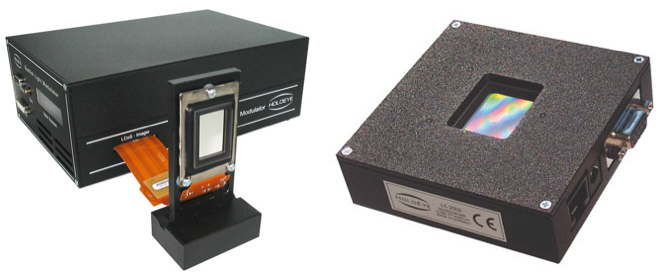
\includegraphics[width=0.5\textwidth]{LCDSLM.png}
\caption[Comparación entre TN-SLM]{Moduladores espaciales modelo PLUTO y LC2012 de reflexión y
  transmisión marca Holoeye basados en la tecnología de cristal
  líquido.}% Por ser fabricado a partir de un LCD comercial el modulador de  la derecha es ensamblado a una cuarta parte del costo del izquierdo.}
\label{fig:LCDSLM}
\end{figure}

Si diferenciamos los SLM por el tipo de tecnología, estos pueden ser
agrupados en dos categorías: basados en cristales líquidos, o en
arreglos de micro espejos (Fig.~\ref{fig:MEMSLM}), mejor 
conocidos en la industria de la proyección como DLP (de Digital Light
Processing).  
\subsubsection{Moduladores basados en micro espejos}
En su mayoría, los moduladores comerciales basados en arreglos de micro
espejos funcionan con micro mecanismos que inclinan una superficie
reflectiva de tal forma que se modifique la cantidad de luz que un
observador ve desde una perspectiva dada, es decir que modulan
intensidad. Sin embargo, con el interés de modular fase además de
intensidad se han desarrollado nuevos micro mecanismos que
permiten desplazar verticalmente el espejo sin modificar su
inclinación, introduciendo así un cambio en la distancia del camino
óptico y por ende, la fase. Tal y como se presenta en los trabajos de
\citetChGen{Wu2010} y \citetChGen{Liesener2006}. Dado que es una
tecnología incipiente y ha tenido menor tiempo en el mercado que los
cristales líquidos, estos sistemas de micromecanismos y en particular los de tipo pistón,
siguen teniendo precios elevados y aún están lejos de ser utilizados
en muchos laboratorios. 
\begin{figure}[h!]
\centering
    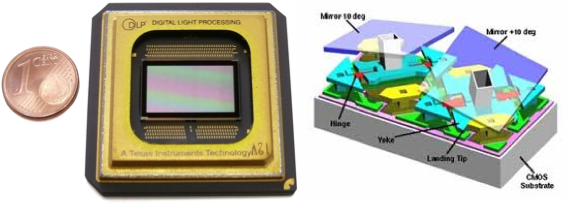
\includegraphics[width=0.5\textwidth]{MEMSLM.png}
\caption[Modulador espacial basado en arreglos de micro espejos]{Modulador espacial basado en arreglos de micro espejos marca Texas Instruments.}
\label{fig:MEMSLM}
\end{figure}

\subsubsection{Moduladores de cristal líquido}
Los SLM basados en Cristales Líquidos (\acrshort{LCs}) aprovechan las propiedades
físicas de ciertos polímeros que dada su forma alargada y propiedades
electrónicas polares, cambian su orientación ante la presencia de
campos eléctricos.  Esta sensibilidad a los campos eléctricos, en
conjunto con sus propiedades ópticas anisotrópicas permitió que desde
los años 70s se implementaran LCs para generar imágenes en pantallas de
dispositivos como relojes, calculadoras y luego televisores y
proyectores. Fue más adelante cuando estudios especializados de las
propiedades de los LCs como los realizados por
\citetChGen{Yeh1999} y \citetChGen{Yariv2002}, y experimentos como los de
\citetChGen{Konforti1988} demostraron que los LCD pueden ser usados
como moduladores de solo fase. Aunque la aplicación de LCs para
modulación de fase es relativamente reciente, el estudio de sus
propiedades físicas no lo es y desde los años 60’s la investigación ha
sido respaldada por grandes empresas interesadas en desarrollar
productos tecnológicos de generación y procesamiento de imágenes como
RTC, Hamamatsu, Hitachi, HP, Texas Instruments, Sony y otros. Dado
el interés por entender los LCs, se ha llegado a modelos matemáticos y  técnicas de  
caracterización robustas que permiten extraer los parámetros de un SLM para
 simular su comportamiento. 
El desarrollo de estas técnicas ha permitido a investigadores 
alrededor del mundo implementar moduladores de fase a
partir de elementos LCD extraídos de dispositivos de proyección
comerciales, entre ellos se encuentran los trabajos de
\citepChGen{Pezzaniti1993,Soutar1994,Zhang1994,Moreno1998,Davis1999,Iemmi2001,Davis2003,Moreno2003,Kim2005,Duran2006,Duran2007,Marquez2007,Liu2010,Ma2010,Ma2011,Yu2012}. Mientras
que autores como Mahmud, \citepChGen{Mahmud2008}, Roopahsree
\citepChGen{Roopashree2009a}, y David \citepChGen{Dev2012}
caracterizaron un Holoeye LC2002 que es vendido comercialmente como
modulador de amplitud y fase.
Ejemplo de la práctica de reensamblar un LCD y venderlo como SLM es el
modulador marca Holoeye LC2012 que gracias a usar un LCD comercial
marca Sony es ensamblado a una cuarta parte del precio de otros
moduladores. 

Adicionalmente, cabe mencionar que los moduladores en base a LCs se
dividen en dos tipos, de reflexión y de transmisión. Sin entrar en
detalle, los primeros permiten modulaciones de fase que van hasta $2\pi$
radianes, tienen mayor resolución, necesitan menos elementos de
polarización para su uso, tienen altas velocidades de operación y el
hecho de que la electrónica esté detrás del cristal (y detrás de la
superficie reflectiva) hace que se produzcan menos efectos indeseados
de difracción. Todo esto a costa de desarrollar LCs y
electrónica personalizados. En cambio, los moduladores de transmisión
se ensamblan a partir de LCs comerciales que fuera de polarizar la luz
retardan su fase. Esto implica un acople entre modulación de fase y 
modulación de intensidad que se traduce en menor calidad de la
modulación de fase total. Para lograr una modulación específica se
necesitan polarizadores y retardadores que generen un 
estado de polarización particular a la entrada del SLM. Por otra
parte, al tener la electrónica acoplada sobre el cristal y no en un
elemento separado como en los de reflexión, se limita la
resolución; no todo el volumen de LC se aprovecha y se introducen
efectos indeseados de difracción. 
No obstante, los SLM de transmisión son muy económicos y algunos
autores como Davis et al. \citepChGen{Davis2000, Davis2013} han propuesto
que se podrían usar como dispositivos para modular polarización. En
base a la idea de usarlos para modular polarización, otros como \citetChGen{Moreno2004, Moreno2011} han
combinado el formalismo de Fourier con el de las matrices de Jones
para modelar el comportamiento de dispositivos ópticos de Fourier que
involucran polarización. 

En el laboratorio de metrología óptica del grupo de Óptica Aplicada de
la Universidad EAFIT se encuentra un moduladores de transmisión
marca Holoeye modelos LC-2002 que en el contexto de este
trabajo ha sido caracterizado para optimizar su uso en aplicaciones metrológicas
tales como la creación y corrección de aberraciones en haces LG.  
La generación de VOs se da entonces de forma expedita una vez se tenga apropiada la
herramienta que los produce.  
A lo largo de este capítulo se presentarán los conceptos teóricos
necesarios para entender la caracterización de SLMs y luego se
presentarán las diversas herramientas y métodos que se implementaron
para lograr la generación de VOs.

% En la sección que sige se introduce la segunda mitad del
% problema, es decir, ¿Cómo caracterizar y corregir las aberraciones ópticas de un VO?

% \subsection{Aberraciones ópticas}

% Los VO generados en el laboratorio están sujetos a aberraciones
% ópticas que se asocian a situaciones tales como:
% \begin{itemize}
% \item Problemas en la alineación de componentes ópticos como
%   lentes o espejos.
% \item Deformaciones en las superficies de elementos como
%   polarizadores, lentes, espejos, láminas retardadoras, e incluso de
%   las céldas de cristal líquido en el SLM.
% \item Presencia de partículas de polvo en las superficies de las
%   componentes ópticas que inducen efectos indeseados de difracción. 
% \end{itemize}

% Adicionalmente, y siguiendo con el tema de la sección anterior, los
% SLM de transmisión basados en pantallas de LC introducen otras fuentes
% de aberraciones. En primera medida, los LCD son dispositivos discretos en dos de los
% sentidos de la palabra; por un lado, son discretos espacialmente y
% las señales de control son asignadas a subdivisiones del cristal de tamaño finito
% conocidas como píxeles. El arreglo rectangular de todos los píxeles
% genera efectos de difracción similares a los de rejillas verticales y
% horizontales combinadas. Esto quiere decir que el SLM separa los
% órdenes de difracción de la luz que pasa a travez de él. Asimismo, el
% hecho de ser una cuadrícula discreta hace que el modulador no pueda
% generar distribuciones de fase en regiones infinitamente pequeñas como
% sería deseado alrededor de una singularidad óptica. Como ejemplo, en la figura
% \ref{fig:discrete_mask} a) se muestra una imagen de la región donde
% resultaría una singularidad óptica en una máscara de
% fase espiral enviada al SLM. Como se puede ver, la máscara de fase
% discreta resulta muy distinta a la máscara ideal presentada en la
% figura \ref{fig:oam_intro}b), y por lo tanto introduce deformaciones
% en el haz Laguerre-Gauss que resulta a la salida del SLM.   

% \begin{figure}[h!]
% \centering
% 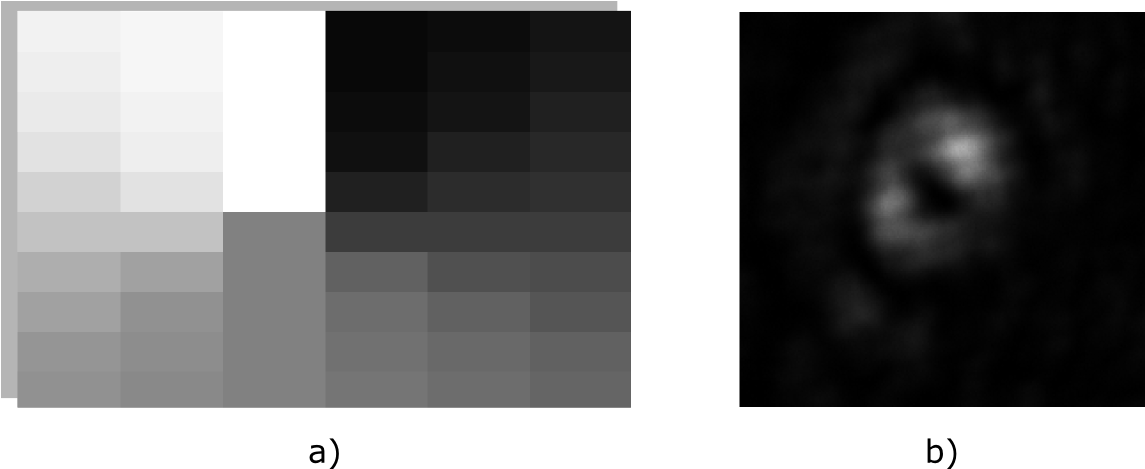
\includegraphics[ scale=.4]{discrete_mask.png}
% %Las imagenes que enviamos al SLM son generadas en un
% %  ordenador que de por sí es discreto, y llegan a un dispositivo
%  % físico que tiene divisiones discretas, tanto espaciales como
%  % electrónicas. Aún 
% \caption[Efecto de pixelado eb el SLM sobre las aberraciones en VO]{a) Magnificación de una mascara tipica proyectada al SLM. b) Imagen de un VO de poca calidad producido con un SLM de
% transmisión modelo Holoeye LC2002.}
% \label{fig:discrete_mask}
% \end{figure}

% Por otra parte, el SLM es discreto en la medida que sólo puede asignar
% níveles de voltaje discretos (0-255 divisiónes de 5V) a cada una de
% las celdas. Este fenómeno también es observable en la figura
% \ref{fig:discrete_mask}a) y puede introducir efectos
% indeseados. Más aún, si cómo el nuestro, el modulador no llega a una
% modulación de sólo fase, o tiene una modulación que no llega a
% completar el ciclo de $2\pi$ radianes. 
% Todas las posibles fuentes de error mencionadas anteriormente se
% combinan para generar haces Laguerre-Gauss de poca calidad como el que se muestra
% en la figura \ref{fig:discrete_mask} b). 


\section{Marco Teórico de la Caracterización de SLMs de Trasmisión}
\label{sec:ChGen_marco_teorico}
\lhead{Generación de haces Laguerre-Gauss por medio de un SLM: \textit{Marco Teórico}}

Dado que los SLMs de transmisión se ensamblan a partir de LCs, lo
primero que hay que tener en cuenta para su caracterización 
es conocer sus generalidades y entender sus propiedades ópticas. 
Entenderemos que los LCs afectan el estado de polarización de la luz y
por ello se dedicará un espacio del marco teórico a presentar los conceptos
generales y herramientas matemáticas propias de la teoría de polarización. 
Una vez presentadas estas herramientas se mostrarán los modelos
actuales con los cuales se representa matemáticamente la modulación de
un LC y se hará una breve revisión de la literatura de la
caracterización de SLMs. 

\subsection{Cristales líquidos}
\subsubsection{Características de los Cristales Líquidos}  
Un cristal Líquido es una sustancia que posee propiedades que
se asemejan tanto a las de los sólidos cristalinos como a las de los
líquidos, y puede ser visto como un líquido en el cual existe
orden entre sus moléculas. Para ilustrar esta idea recordemos que los
sólidos cristalinos son un estado de la materia que se caracteriza por
su rigidez y fuertes enlaces químicos, en el cual se puede
establecer un orden posicional en todas las direcciones tal y como se
ilustra en la Fig.~\ref{fig:solido}. Esto implica que la posición de
las moléculas o átomos que lo componen puede ser abstraída como una
red periódica que cumple ciertas reglas de simetría. En cambio, un
líquido amorfo como el de la Fig.~\ref{fig:liquido} tiene enlaces
más débiles por lo cual puede fluir y está compuesto
por moléculas que están completamente desorganizadas. 
\begin{figure}[h!]
\centering
\begin{subfigure}{.45\textwidth}
  \centering
  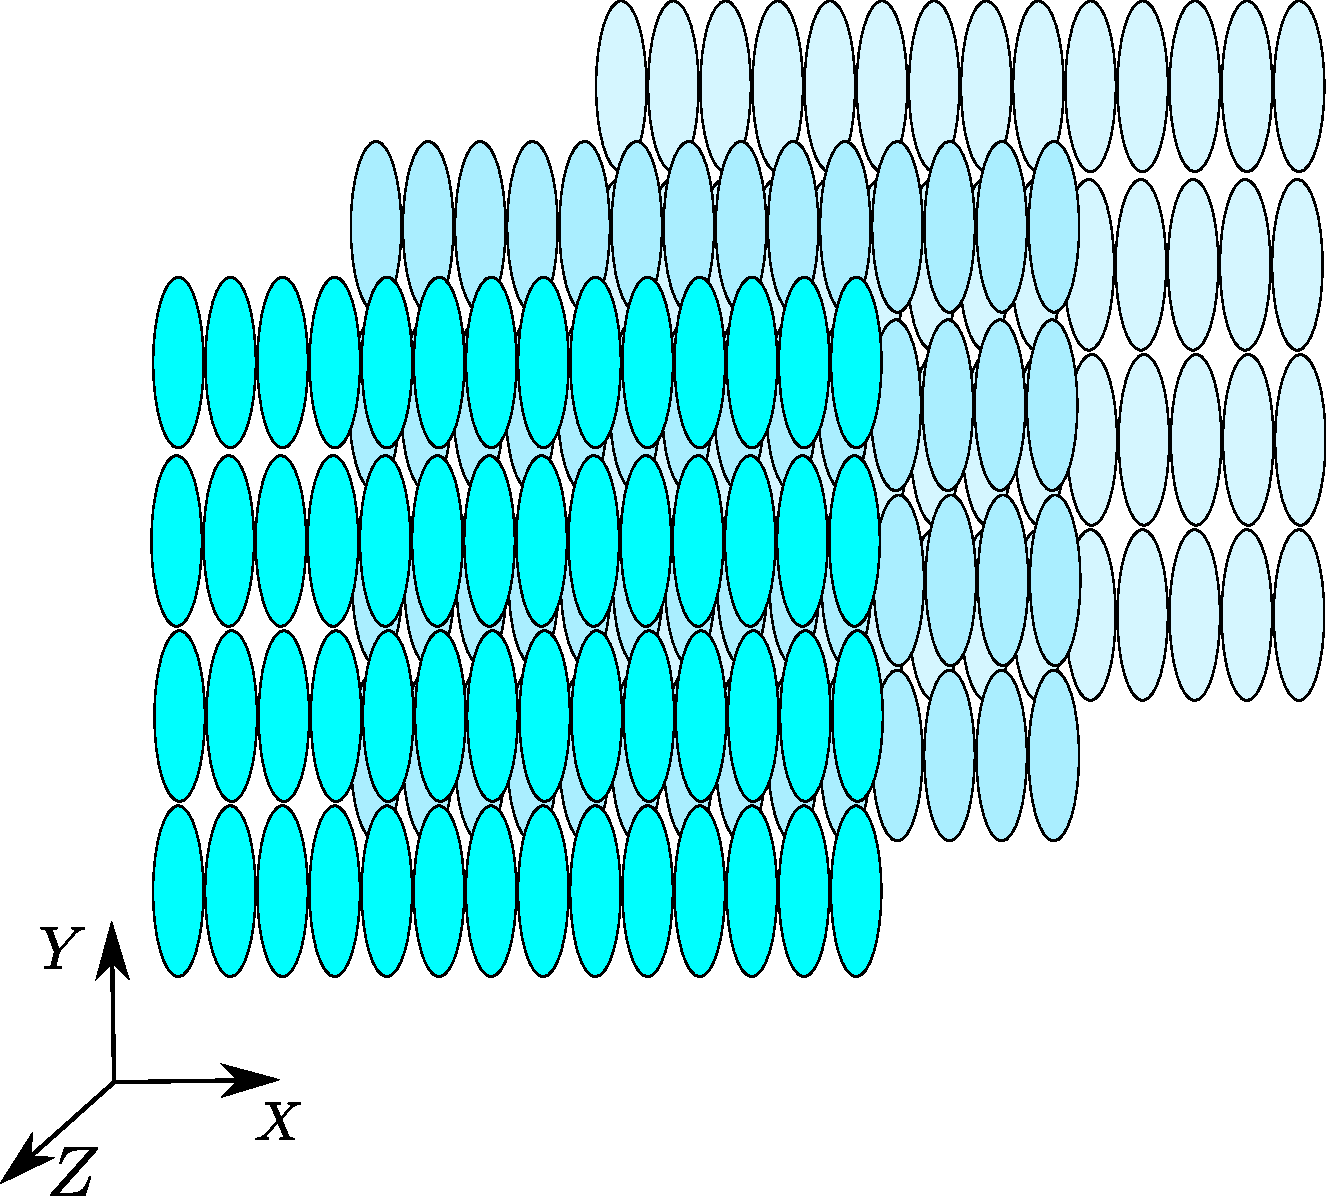
\includegraphics[width=.6\linewidth]{Cristaline_solid}
  \caption{Moléculas con orden posicional y orientacional en un sólido cristalino.}
  \label{fig:solido}
\end{subfigure}\qquad
\begin{subfigure}{.45\textwidth}
  \centering
  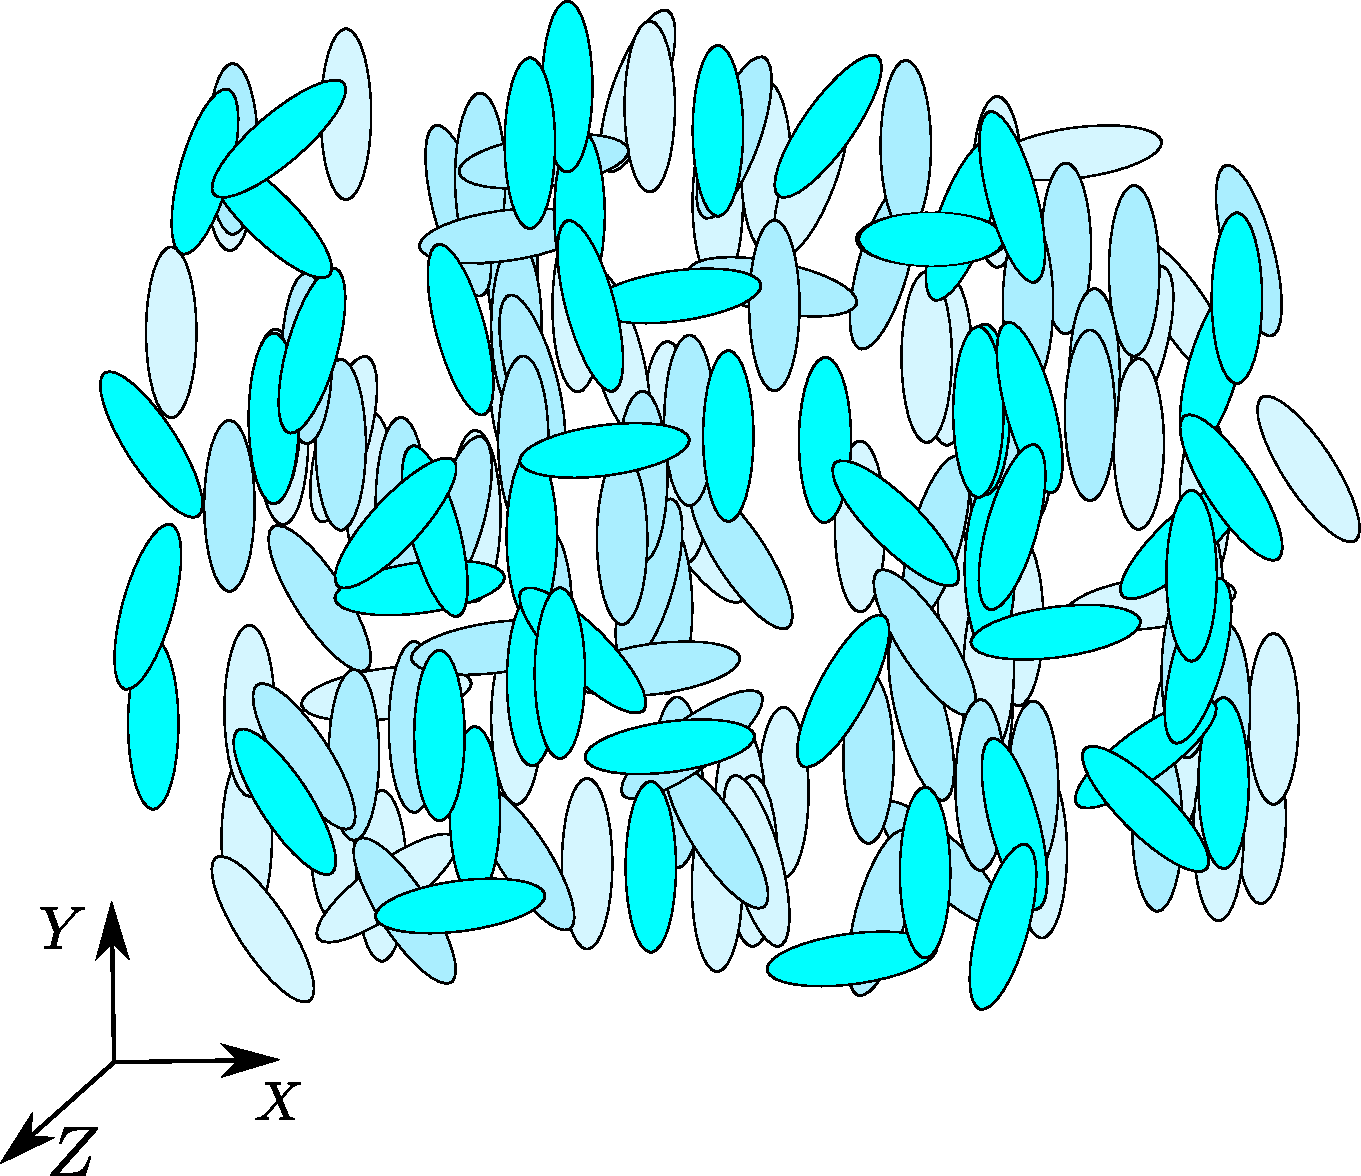
\includegraphics[width=.6\linewidth]{liquid}
  \caption{Moléculas desordenadas pero cercanas en un líquido.}
  \label{fig:liquido}
\end{subfigure}
\caption{Dos estados de la materia comunes en la naturaleza.}
  \label{fig:estados}
\end{figure}

Los cristales líquidos son sustancias que como los
sólidos poseen cierto orden y que pueden fluir como los líquidos. 

Por otra parte, los LCs pueden ser clasificados en tres tipos o fases distintas
conocidas como, \textit{nemáticos},
\textit{smeticos} y \textit{colestéricos}, y más adelante se abordará esta
clasificación. No obstante su diversidad (más de 100.000 compuestos
distintos según \url{http://www.lci-publisher.com}), la característica
común de los LCs es que están 
compuestos de moléculas altamente anisotrópicas, esto es, que sus
propiedades (ópticas, eléctricas y mecánicas) dependen de la
dirección desde la que se observen. La anisotropía se debe tanto a la
geometría alargada o achatada de las moléculas, como a las propiedades
electrónicas de sus componentes \citepChGen{Gennes1995,Yeh1999,Yariv2002}. En el caso de moléculas
alargadas de LCs como la de la Fig.~\ref{fig:LCMolecule} la
estructura química de un LC general se
compone de un sistema de anillos aromáticos que pueden ser o no
saturados conectados por un grupo de conexión A, y sujetos a dos
cadenas o grupos terminales X y Y \citepChGen{Yeh1999}. 
\begin{figure}[h!]
\centering
    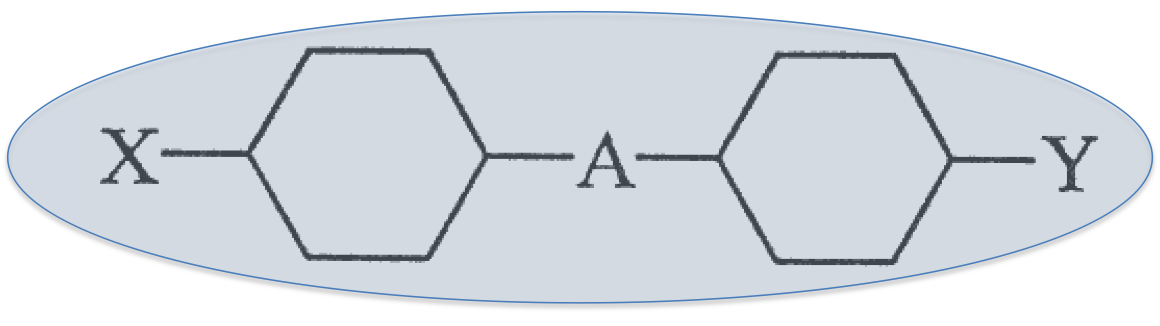
\includegraphics[width=0.5\textwidth]{LCMolecule}
\caption{Esquema de la composición química general en una molécula de LC.}
\label{fig:LCMolecule}
\end{figure}

La presencia de los anillos proporciona las fuerzas intermoleculares de corto alcance que
son necesarias para formar fases nemáticas y el tipo de anillos
(saturado o no saturado) determina la presencia o no de enlaces $\pi$
que se asocian a orbitales $P_z$ de los electrones. Esto a su vez
afecta la absorción en el ultravioleta y la birefringencia; se observa mayor
birefringencia en LCs con anillos no saturados y mejor comportamiento
en el ultravioleta para anillos saturados \citepChGen{Gennes1995}.  Luego, las cadenas del
grupo terminal X pueden ser de tres tipos,
\begin{itemize}
\item Cadenas alquilos (alkyl)  $C_nH_{2n+1}$,
\item Grupos alcoxy $C_nH_{2n+1}O$,
\item Grupos alilos (alkenyl) $CH_2=CH-CH_2-$.
\end{itemize}
 La longitud de las cadenas X influencia tanto las constantes elásticas
 como las temperaturas de transición de fase. Para cadenas cortas con
 uno o dos átomos de carbono los grupos son muy cortos como para
 presentar fases de LC. Los grupos terminales de tamaño medio: n = 3-8
 son los más adecuados para construir fases nemáticas por su
 mayor anisotropía, y los compuestos con cadenas aún más largas
 exhiben fases smeticas. La temperatura a la cual la solución pasa de
 ser nemática a isotrópica se conoce como el punto de aclarado o
 \textit{clearing point}, en términos generales, esta temperatura
 disminuye en la medida en la que se alargan los tamaños del 
 grupo terminal X. La función que relaciona el punto de aclarado con
 el número de átomos de carbono es una función suave en la cual los
 números pares generan temperaturas más bajas que los impares. Fuera
 de esto, las propiedades mecánicas como la viscosidad también se ven
 afectadas por el tamaño de los grupos terminales, cadenas
 largas implican viscosidades más altas, y por ello frecuencias de
 operación más bajas \citepChGen{Gennes1995}. 
Finalmente, las cadenas que forman el grupo terminal Y son las que
tienen mayor influencia en las constantes dieléctricas de la molécula
($\epsilon_x,\epsilon_y$), y asimismo su anisotropía dieléctrica
$\Delta\epsilon$ variables que como veremos más adelante son las que
determinan la birrefringencia del LC asociada a la modulación de fase.
Las cadenas del grupo terminal Y pueden ser:
\begin{itemize}
\item No polares: No Influencian mucho la anisotropía dieléctrica, un
  ejemplo es el grupo alquilo $CnH2n+1$.
\item Polares:  Como CN, F, y Cl. Su alta polaridad induce en la
  molécula una alta anisotropía dieléctrica y por tanto alta
  birrefringencia. La alta anisotropía se obtiene a costa de alta viscosidad, resistividad
  insuficiente y problemas de estabilidad bajo iluminación 
  ultravioleta. Los grupos Y muy polares como los que contienen
  cianuro CN No son buenos para operar a  altas temperaturas como por
  ejemplo proyectores, y sufren de degradación en el UV. Para esas
  aplicaciones se utilizan compuestos menos polares como el flúor o
  cloro que tienen menor birrefringencia \citepChGen{Gennes1995}.
\end{itemize}

\subsubsection{Clasificación de los LC}  
\label{sec:LC-clasification}
En 1922 y sintetizando los hallazgos de 30 años desde el descubrimiento
de los LCs, el cristalógrafo George Friedel publicó un artículo \citepChGen{Friedel1922}
en el que clasifica los LCs en tres tipos básicos conocidos como
cristales smeticos, nemáticos y colestéricos.
En términos de orden, los LCs sméticos son los más similares a un
sólido, y los nemáticos se asemejan más a un líquido, y en la medida
en la que se calienta un LC éste realiza una transición desde cristal
smetico hasta líquido isotrópico pasando por la fase nemática. Los estados
colestéricos son un tipo particular de LCs nemáticos que a diferencia
de los anteriores tienen propiedades inhomogeneas. 
La principal característica que le da una medida de orden a los LCs es
la tendencia de sus moléculas a orientarse en una dirección
preferente gracias a su distribución polar de cargas. Esta tendencia
se puede observar claramente en las figuras \ref{fig:smetic} y
\ref{fig:nematic} como si las moléculas fueran vagones de un tren que
se siguen uno detrás del otro en forma de hilo \footnote{La palabraa
\textit{Nematic} proviene de la expresión griega \textit{nema} que
significa hilo.}.  

La orientación preferencial de las moléculas les
otorga una cierta medida de orden a los LCs que en adelante llamaremos orden
orientacional. La \textit{cantidad} de orden se medirá por medio de un
parámetro estadístico conocido como parámetro de orden, que relaciona
la orientación de las moléculas individuales con la orientación
preferencial o vector director $\vec{n}$ en las vecindades de
la molécula. Si se tiene un conjunto de moléculas como la que se
ilustra en la Fig.~\ref{fig:angulo_director} dónde 
$\theta$ es el ángulo que se forma entre el eje mayor de la molécula
$\vec{v}$ y el vector director, el parámetro de orden orientacional
del cristal se da como el siguiente promedio estadístico sobre todas
las moléculas.

$$ S = \frac{1}{2}\left<3\cos^2{\theta-1}\right>$$
 
\begin{figure}[h!]
\centering
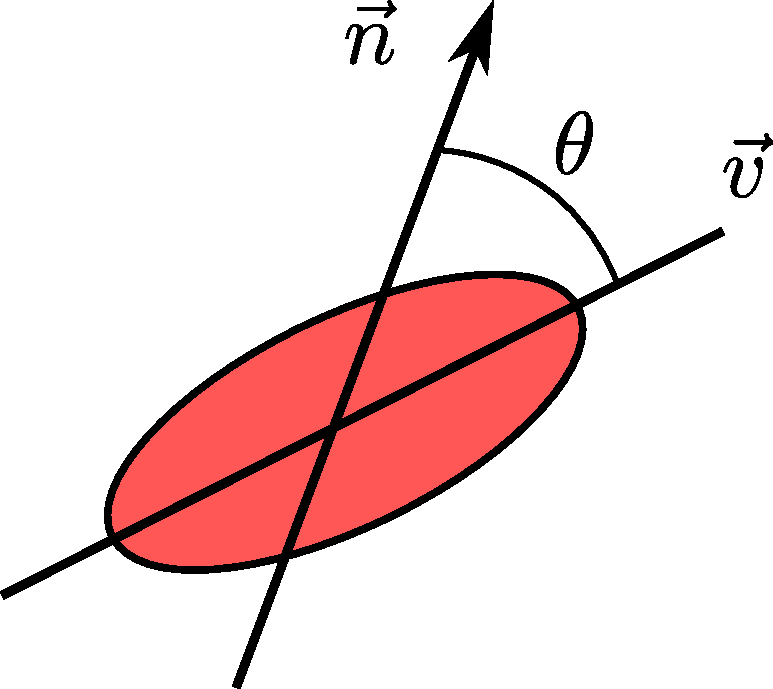
\includegraphics[width=.3\linewidth]{angulo_director}
\caption{Orientación de una molécula de LC con respecto al ángulo
  director en su vecindad.}
\label{fig:angulo_director}
\end{figure}

Un LC con sus moléculas alineadas perfectamente paralelas tiene un
parámetro de orden $S=1$, mientras que un LC con moléculas orientadas
aleatoriamente posee un parámetro $S=0$. El parámetro de orden depende
tanto del tipo de molécula como de la temperatura; en la medida en la
que aumenta la temperatura las moléculas pierden su alineación y el LC
se convierte en un líquido isotrópico. El parámetro de orden gana
importancia cuando se necesita seleccionar un LC que deba ser usado en
rangos de temperatura especiales y se necesite garantizar anisotropía.

\begin{figure}[h!]
\centering
\begin{subfigure}{.4\textwidth}
  \centering
  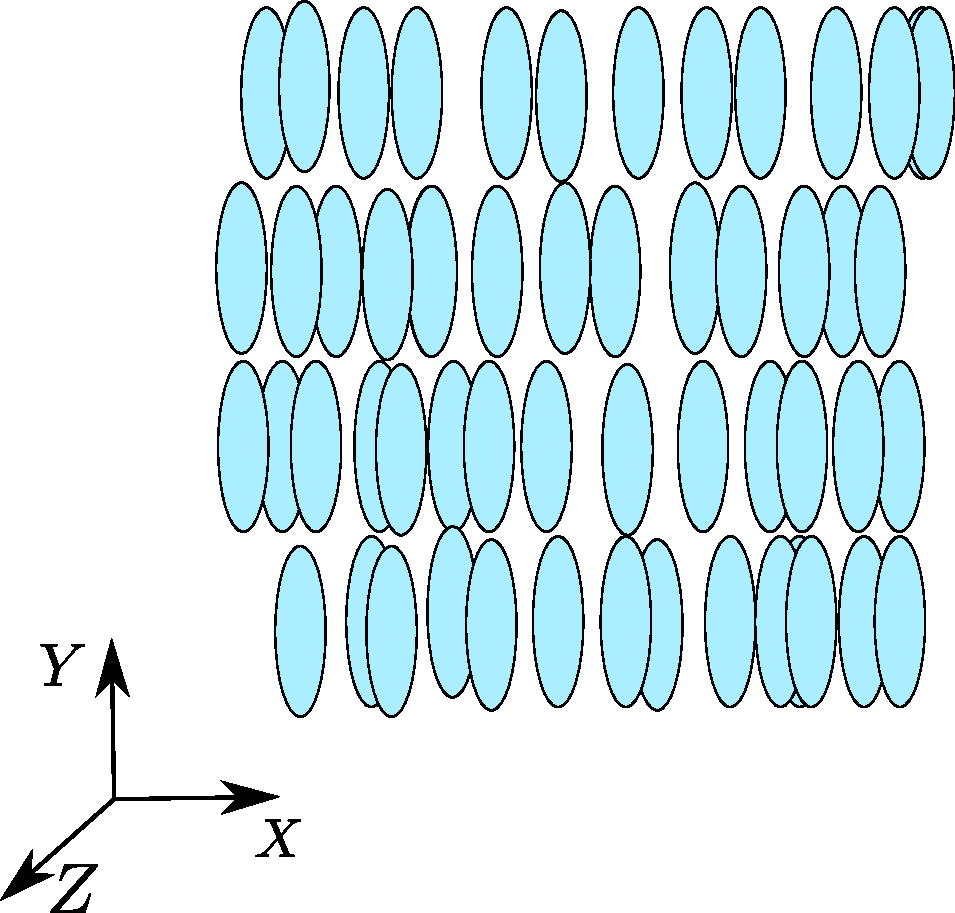
\includegraphics[width=.6\linewidth]{Smetic_LC}
  \caption{Cristal líquido smético.}
  \label{fig:smetic}
\end{subfigure}\qquad
\begin{subfigure}{.4\textwidth}
  \centering
  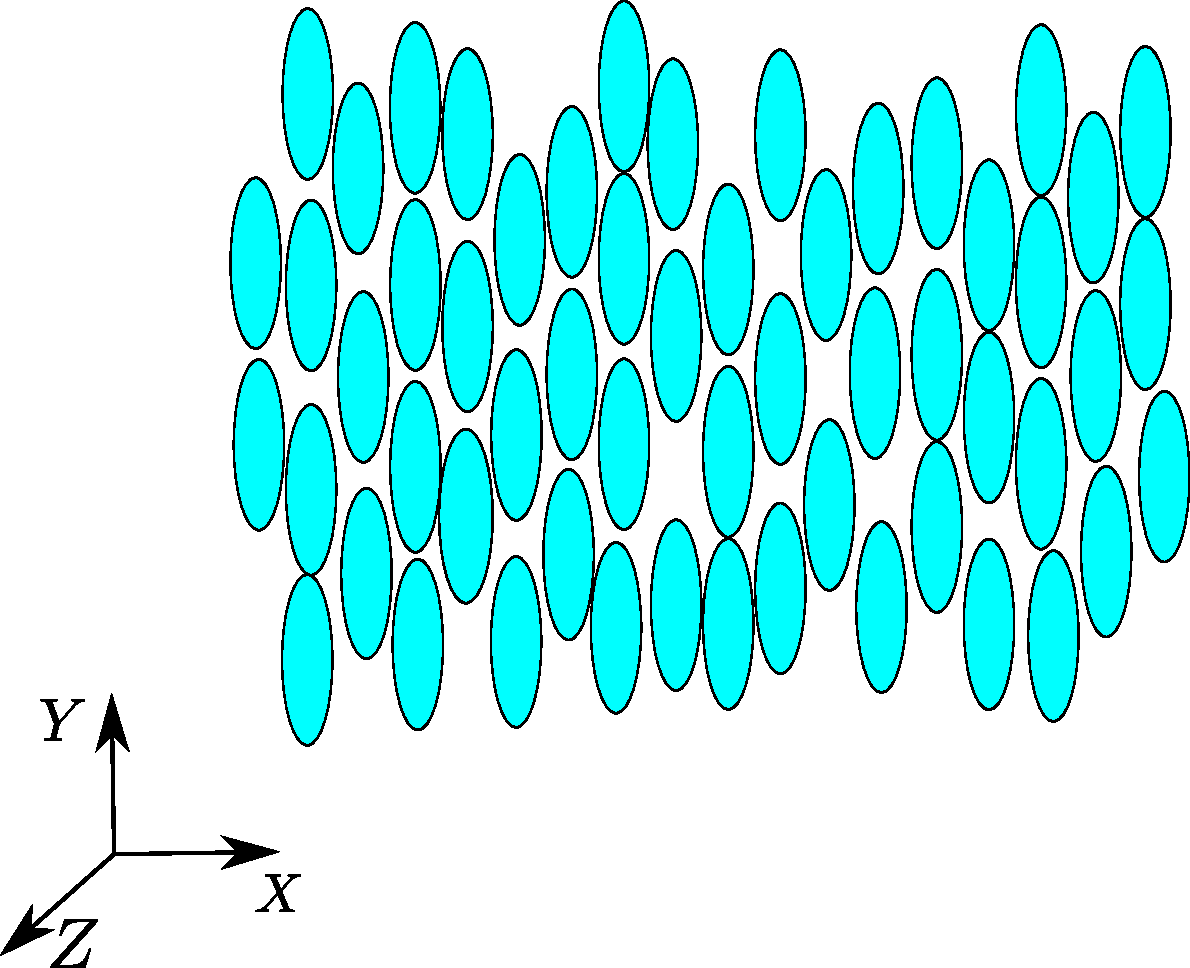
\includegraphics[width=.6\linewidth]{Nematic_LC}
  \caption{Cristal líquido nemático.}
  \label{fig:nematic}
\end{subfigure}\\
\begin{subfigure}{.5\textwidth}
  \centering
  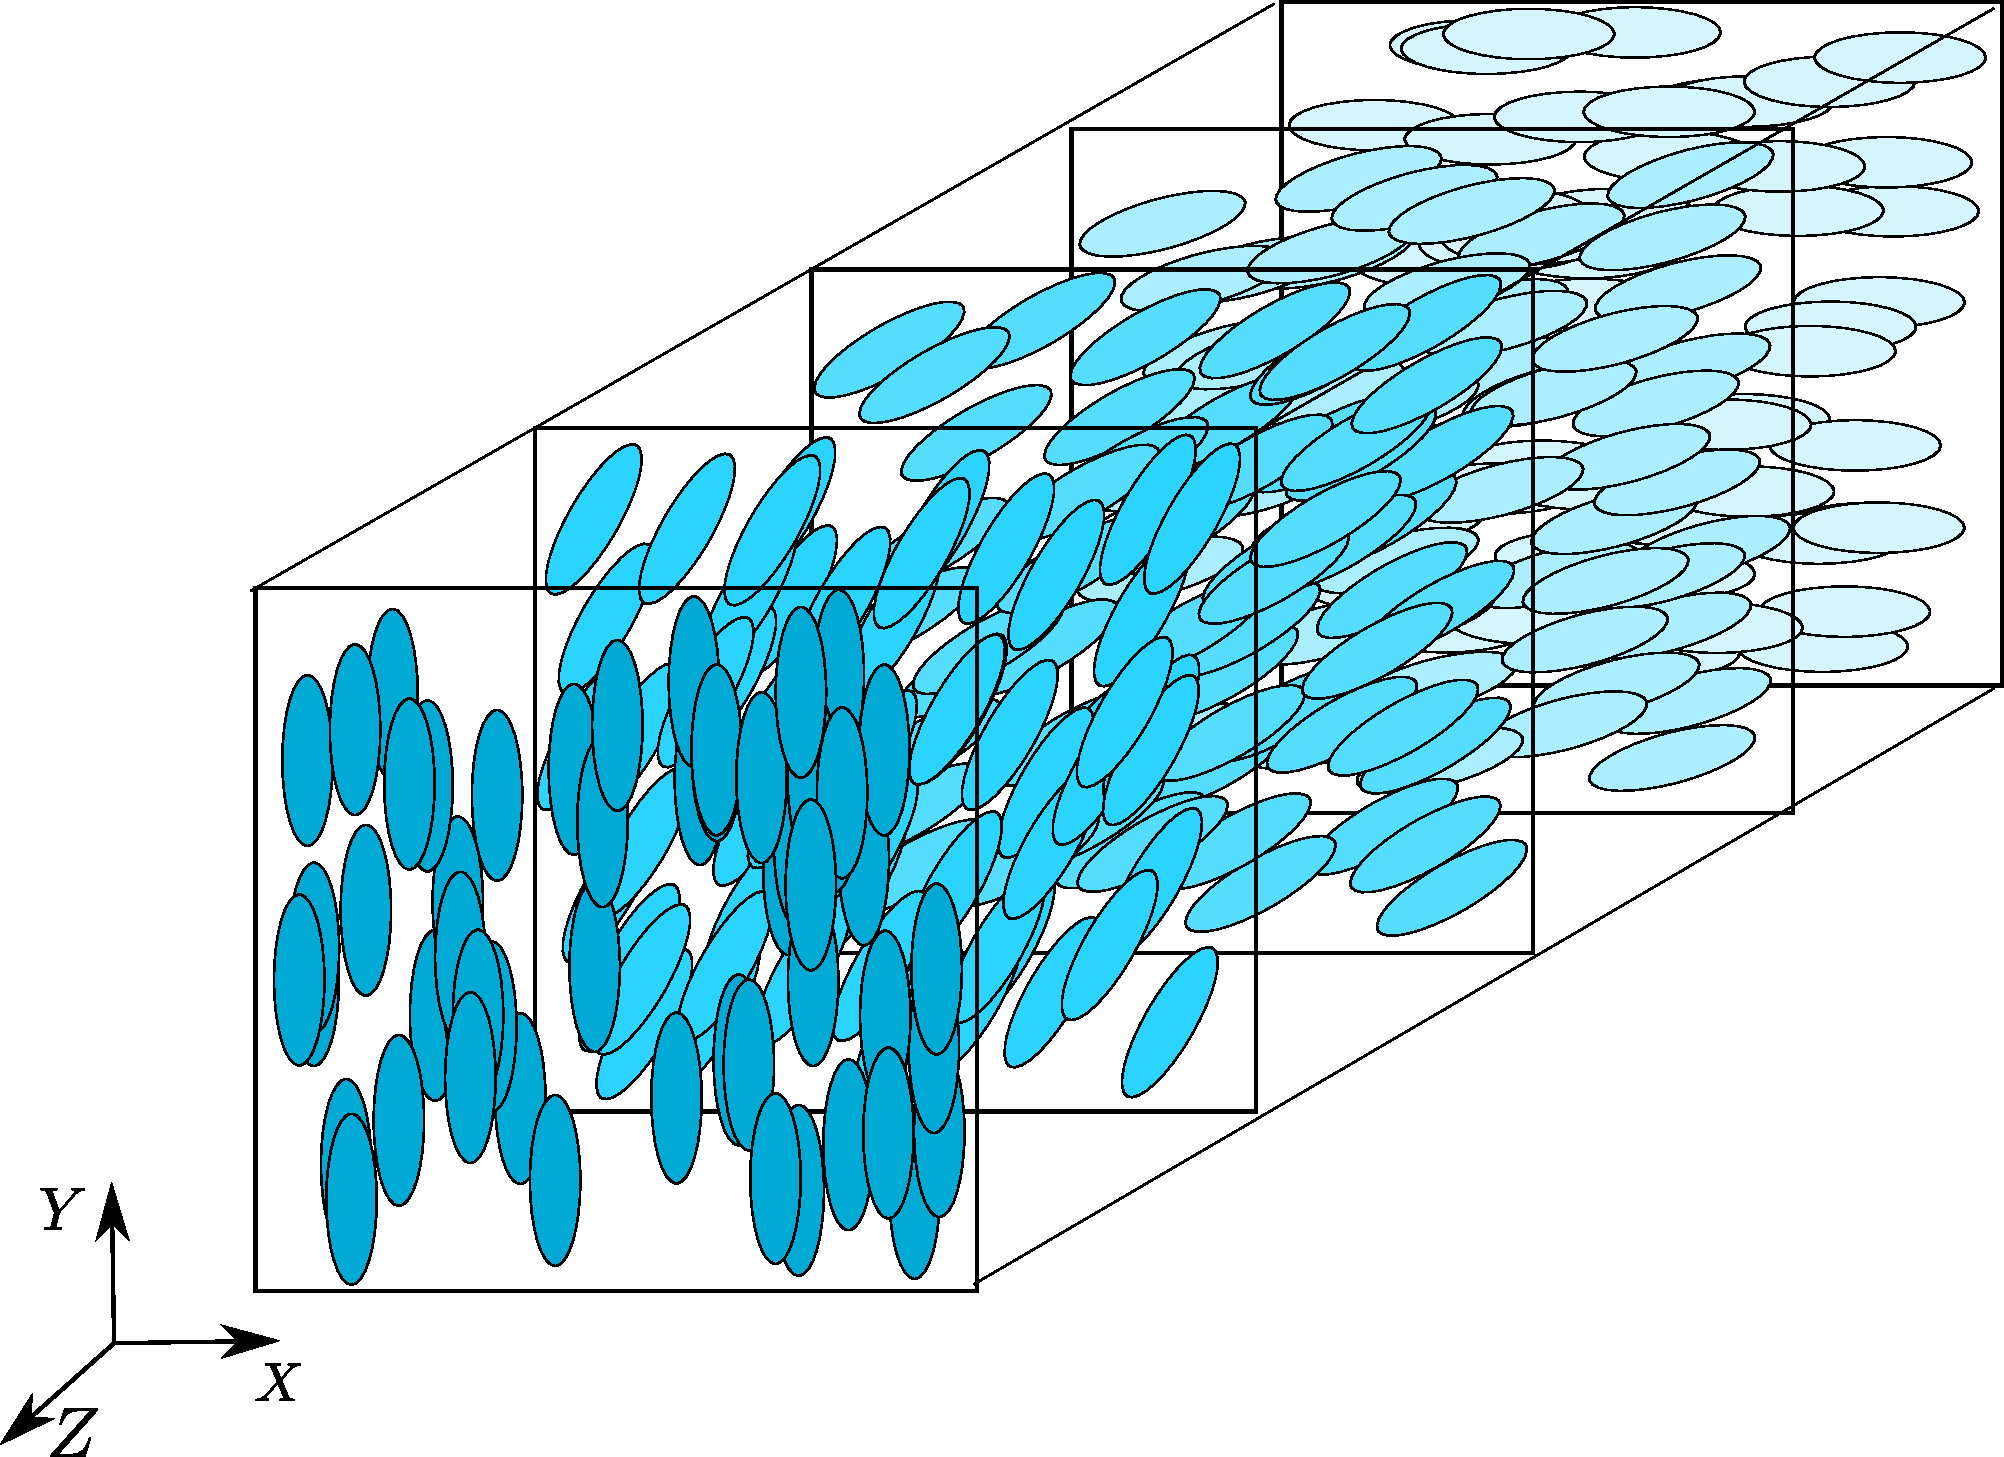
\includegraphics[width=.6\linewidth]{Cholesteric_LC_2}
  \caption{Cristal líquido colestérico.}
  \label{fig:cholesteric}
\end{subfigure}
\caption{Clasificación de los cristales líquidos según su orden.}
\label{fig:CL_clasificacion}
\end{figure}

Los Cristales smeticos como el que se ilustra en la Fig.~
\ref{fig:smetic} se diferencian de los nemáticos en que poseen orden
posicional en una dirección además de orden orientacional. Sin embargo,
este orden viene acompañado de propiedades mecánicas que son menos
convenientes para la construcción de LCDs y por ello las fases
nemáticas y colestéricas son las que tienen mayor número de
aplicaciones en dispositivos electro ópticos. 
A diferencia de las fases smetica y nemática que tienen un solo vector
de orientación, en los cristales líquidos colestéricos el vector
director varía a través del medio de una forma bien
definida y por ello se consideran medios inhomogeneos. Generalmente la
variación es helicoidal como la que se ve en la Fig.~\ref{fig:cholesteric}.   
La variable que caracteriza un cristal líquido colestérico es el
ángulo de inclinación o pitch que forman las moléculas inclinadas con
respecto al eje óptico del material. 


\subsubsection{Las pantallas de cristal líquido nematico retorcido.}


Los moduladores de LC de transmisión que se usan para proyección se
construyen usando una configuración conocida como \textbf{Twisted
Nematic} (\acrshort{TN-LCD}) o nemáticos retorcidos. Los TN-LCD son
dispositivos como el que se ilustra en la Fig.~\ref{fig:tn-lcd} en
los cuales una  solución de cristal líquido nemático se inyecta entre
dos superficies rígidas transparentes que han sido rayadas o frotadas
a lo largo de una dirección preestablecida. Este proceso se conoce
rayado direccional. Las moléculas del LC en
contacto con las superficies transparentes se adhieren a los canales
microscópicos que resultan del rayado, tomando así una
dirección preferencial en ese plano. Cuando las 
direcciones de rayado de las superficies en ambos extremos no
coinciden, la dirección preferente de orientación de las moléculas
cambia gradualmente en profundidad desde la dirección del plano de
entrada hasta la del plano de salida como se ve en la Fig.~
\ref{fig:tn-lc}.  El resultado es un cristal líquido inhomogeneo
parecido a un cristal colestérico en el cual la orientación de las
moléculas varía de forma lineal.

\begin{figure}[h!]
\centering
\begin{subfigure}{.45\textwidth}
  \centering
  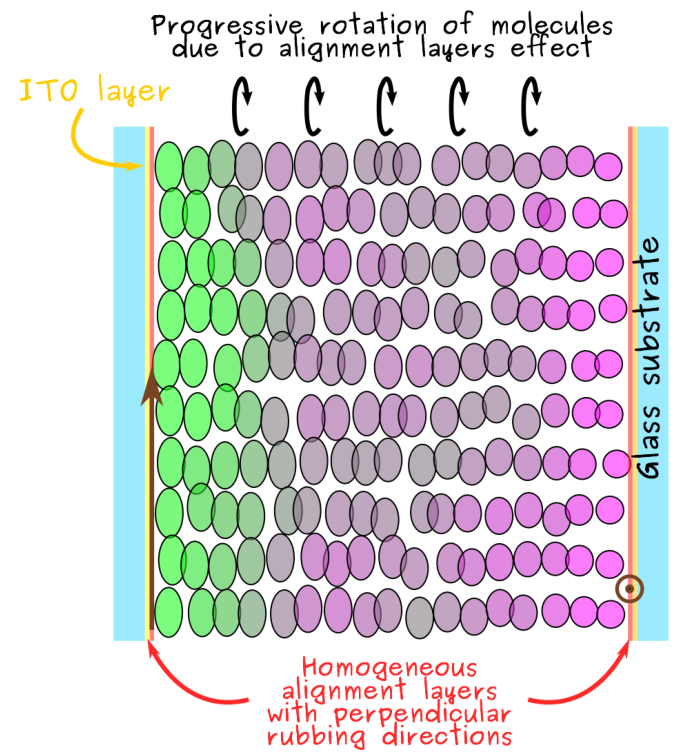
\includegraphics[width=.8\linewidth]{tn-lcd}
  \caption{Esquema de un TN-LCD cuando no hay un voltaje entre las placas.}
  \label{fig:tn-lc}
\end{subfigure}\qquad
\begin{subfigure}{.45\textwidth}
  \centering
  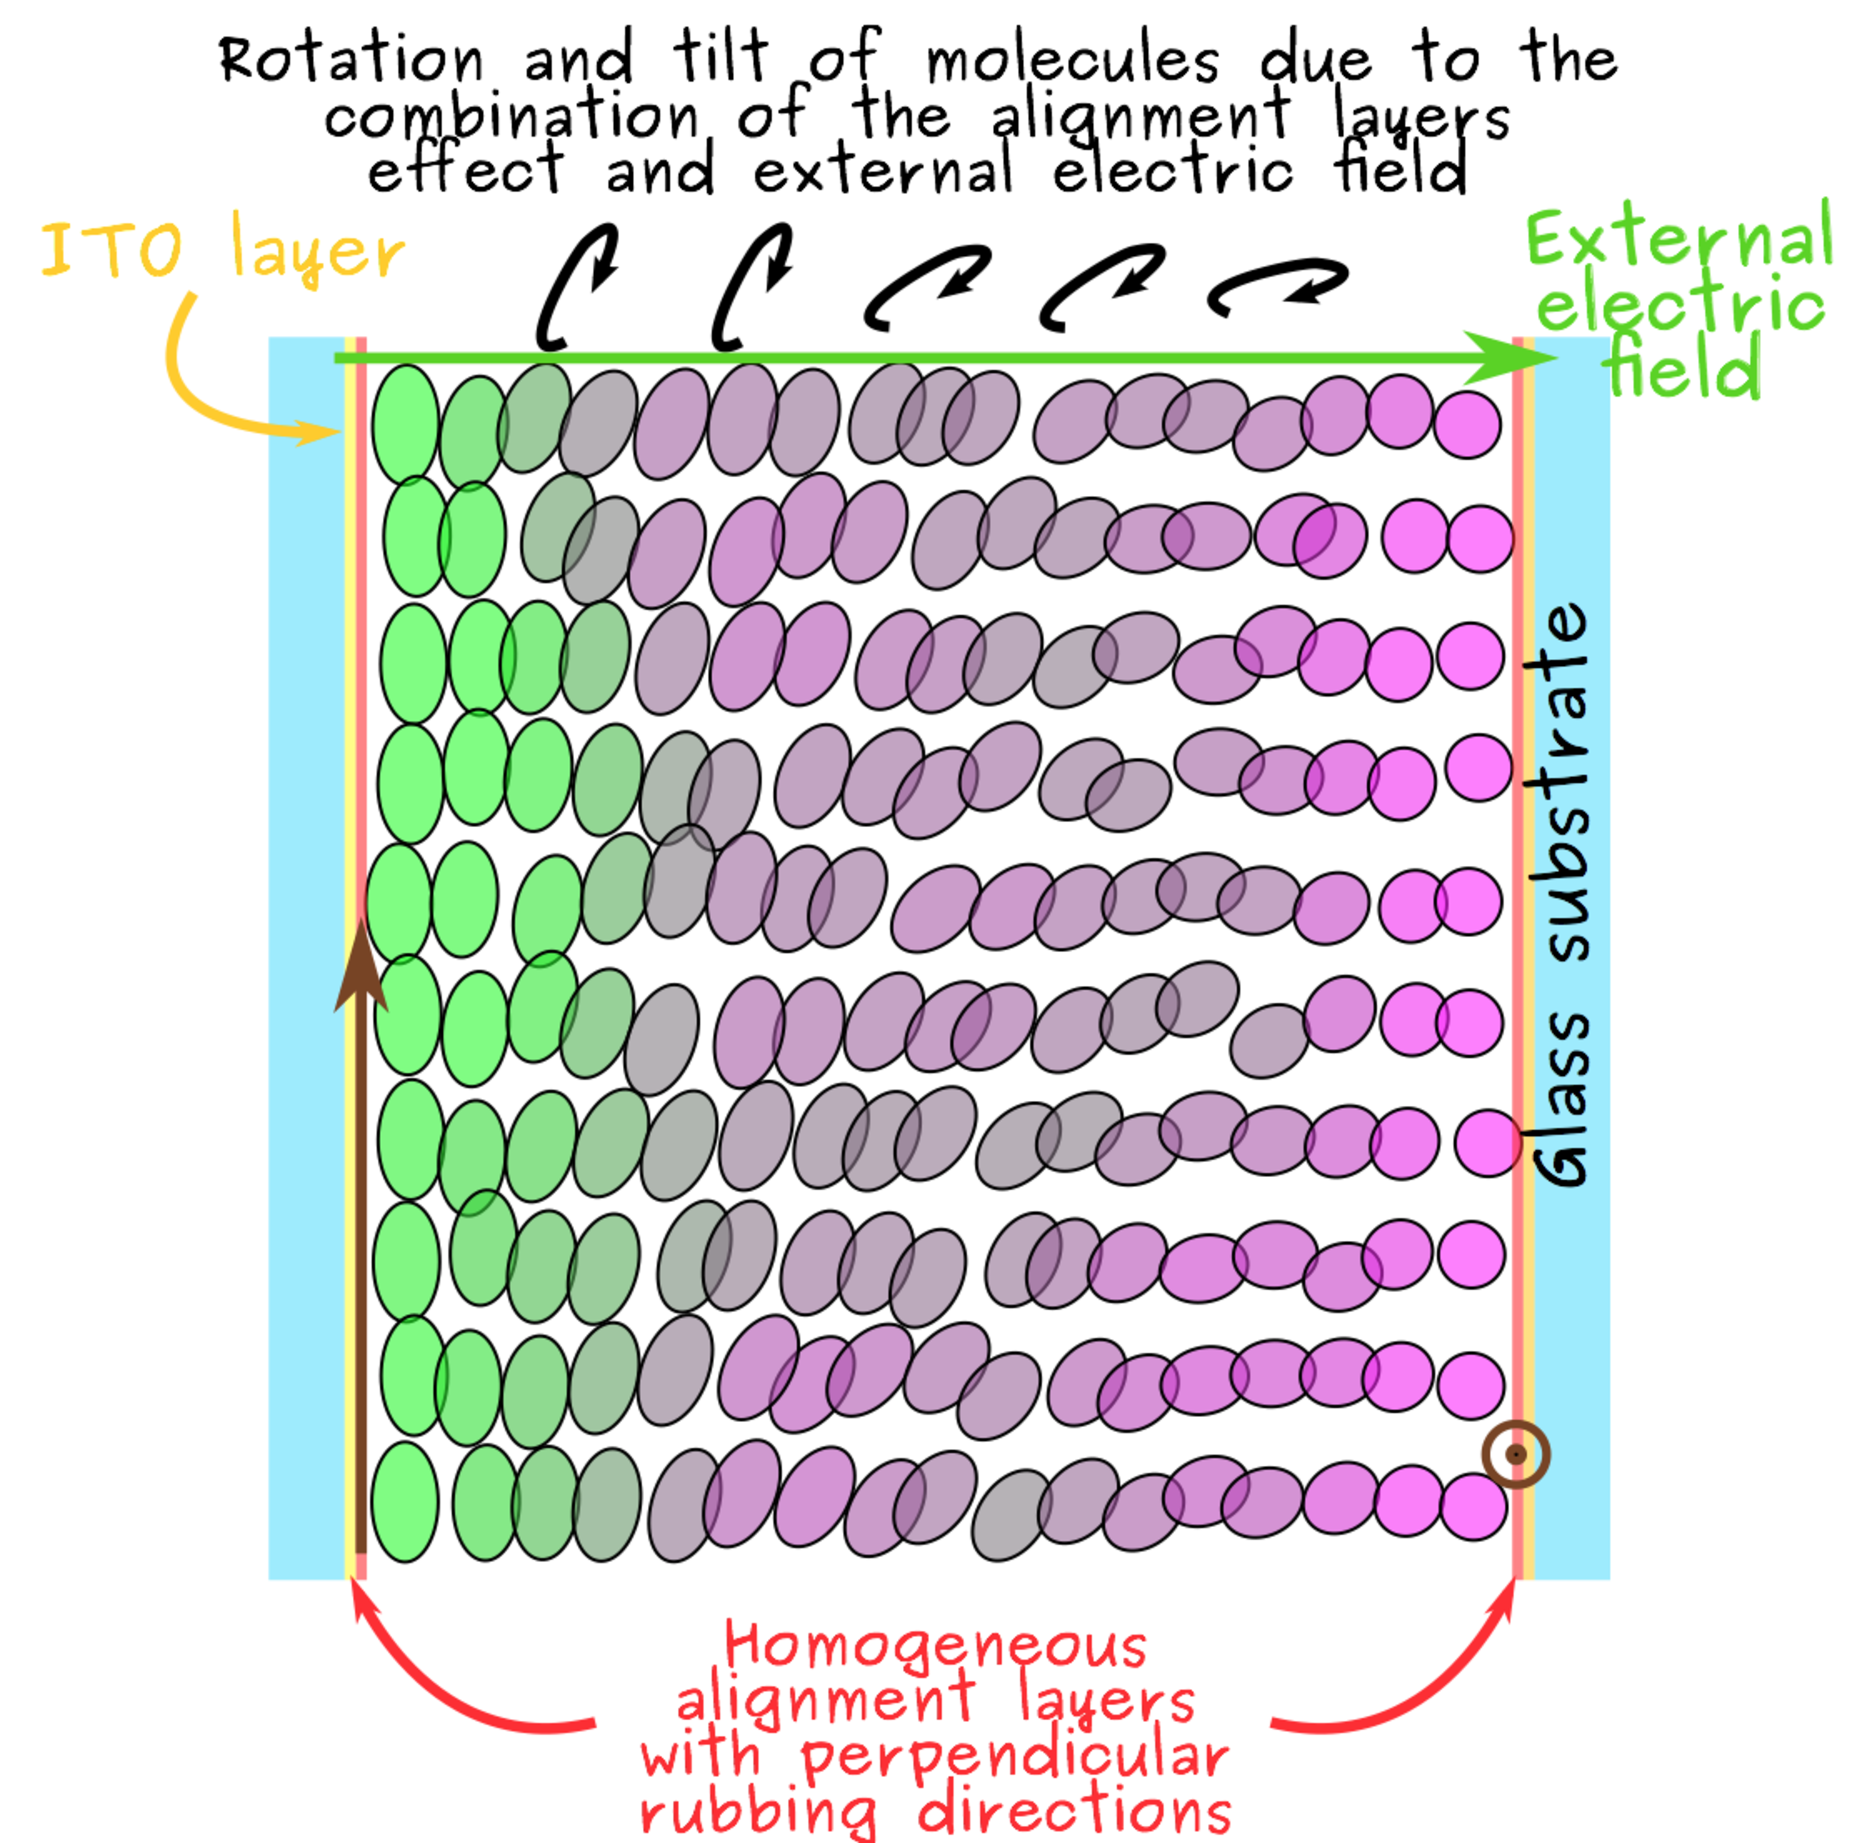
\includegraphics[width=.8\linewidth]{tn-lcd-voltage}
  \caption{Esquema de un TN-LCD dónde se aplica una diferencia de
    potencial entre placas}
  \label{fig:tn-lc-voltage}
\end{subfigure}
\caption[Arquitectura de un TN-LCD]{Arquitectura de un TN-LCD cuando (a) está apagado, y (b) se
  le aplica una diferencia de potencial. Tomado de Nestor Uribe \citepChGen{UribePatarroyo2011}}
  \label{fig:tn-lcd}
\end{figure} 

Generalmente las direcciones de frotado en las superficies de entrada
y salida son ortogonales de tal forma que las moléculas a la salida experimentan
una rotación de 90 grados con respecto a las de la entrada. Ante la
presencia de un campo eléctrico a lo largo del cristal las moléculas
experimentan una inclinación que es proporcional a la diferencia de
potencial entre las placas tal y como se ilustra en la Fig.~
\ref{fig:tn-lc-voltage}. Al ser moléculas alargadas y polares
experimentan un torque que atrae a la parte negativa de la molécula
hacia el electrodo positivo del  dispositivo y viceversa. La
inclinación es proporcional al voltaje aplicado y es de mayor magnitud
en las regiones más alejadas de las paredes del dispositivo. La
configuración TN ha sido seleccionada para muchos
dispositivos electro ópticos comerciales porque afecta 
la polarización de la luz que incide sobre ella. El objetivo de los
autores que han caracterizado moduladores de transmisión ha sido
principalmente el de describir matemáticamente y de forma robusta las
propiedades ópticas de dispositivos que tienen cristales líquidos de
esta naturaleza.  

En lo que sigue se presentarán las herramientas que son
base para la descripción matemática de campos ópticos polarizados, y
se aplicará para la construcción de un modelo de TN-LCD.

\subsection{Polarización de la luz}

En la teoría electromagnética de la luz se representan los campos
ópticos como ondas que se propagan en el espacio vacío. Un haz de luz
se puede representar tanto por su vector de campo eléctrico como
magnético y ambos son perturbaciones de carácter periódico. Si el
medio de propagación es isotrópico, la dirección de la perturbación 
es transversal, es decir ortogonal a la dirección de propagación
($\mathbf{k}\cdot\mathbf{E}$). Para haces planos monocromáticos se
suele usar la siguiente expresión para el campo eléctrico:  

\begin{align}
\mathbf{E} &=\Re\left[\mathbf{A}e^{i\left( \omega t -\mathbf{k}\cdot \mathbf{r}\right)}\right]\label{eq:complex_field},\\
\mathbf{E} &=\mathbf{A}\cos{ \left(\omega t -\mathbf{k}\cdot
    \mathbf{r}\right)},\notag
\end{align}
dónde, $i = \sqrt{-1}$, $\omega$ es la frecuencia temporal, $\mathbf{k}$ es el vector de
onda o frecuencia espacial, y $\mathbf{A}$ determina la amplitud.
Las frecuencias espacial y temporal se relacionan por medio de la
longitud de onda  ($\lambda$) y el índice de refracción del medio ($\mathbf{n}$) con la
siguiente expresión:

$$\mathbf{k} = \mathbf{n} \frac{2\pi}{\lambda}.$$

Dado que son ortogonales, las variaciones del campo se pueden
representar sobre un plano que es 
ortogonal a la dirección de propagación ($z$ en nuestro caso), y ese plano se puede
representar a su vez por dos vectores que son ortogonales entre si
($x$, $y$).
Cuando la variación del campo sucede sobre una dirección preferencial
se dice que la luz es polarizada, y esa dirección se puede descomponer
como una combinación lineal de las variaciones mutuamente independientes
sobre cada uno de los ejes que forman el plano:

\begin{align}
\mathbf{E} &= E_x +E_y, \notag\\
E_x &= A_x\cos{ \left(\omega t -kz+\delta_x\right)} \label{eq:xcomp},\\
E_y &= A_y\cos{ \left(\omega t -kz+\delta_y\right)}\label{eq:ycomp}.
\end{align}

Se ha separado entonces el campo en sus componentes vertical ($y$) y
horizontal ($x$), cada una con su respectiva amplitud ($A_x,A_y$) y
retardo en fase ($\delta_x,\delta_y$). Dado que las amplitudes son
positivas las fases se dan en el rango $-\pi<\delta_{x,y}<\pi$.
La representación en componentes perpendiculares se asemeja a un
sistema acoplado de osciladores armónicos que oscilan a una misma
frecuencia. Si se dibuja la suma vectorial de las componentes $x$, y $y$ como
un vector que va desde el origen hasta el punto ($E_x,E_y$) y luego se
avanza en el tiempo, la trayectoria que describe la punta del vector
será una curva elíptica como la que 
se muestra en la Fig.~\ref{fig:ellipse_clean} . Si en cambio se congela el tiempo y se gráfica
el desplazamiento de la punta del vector en el espacio se obtiene una curva
helicoidal como en la Fig.~\ref{fig:trayectory_clean}. En estos dibujos se ha
escogido representar una elipse por que es el caso más general de polarización. Sin
embargo, la relación entre las amplitudes ($A_y/A_x$) y la
diferencia de fases ($\delta = \delta_y-\delta_x$) entre las componentes del
campo determina si la polarización es lineal ($\delta = 0$), circular
($\delta =\pm \frac{\pi}{2}, A_y/A_x=1$) o elíptica, y la orientación del eje
mayor de la elipse con respecto al eje $x$.

\begin{figure}[h!]
\centering
\begin{subfigure}{.45\textwidth}
  \centering
  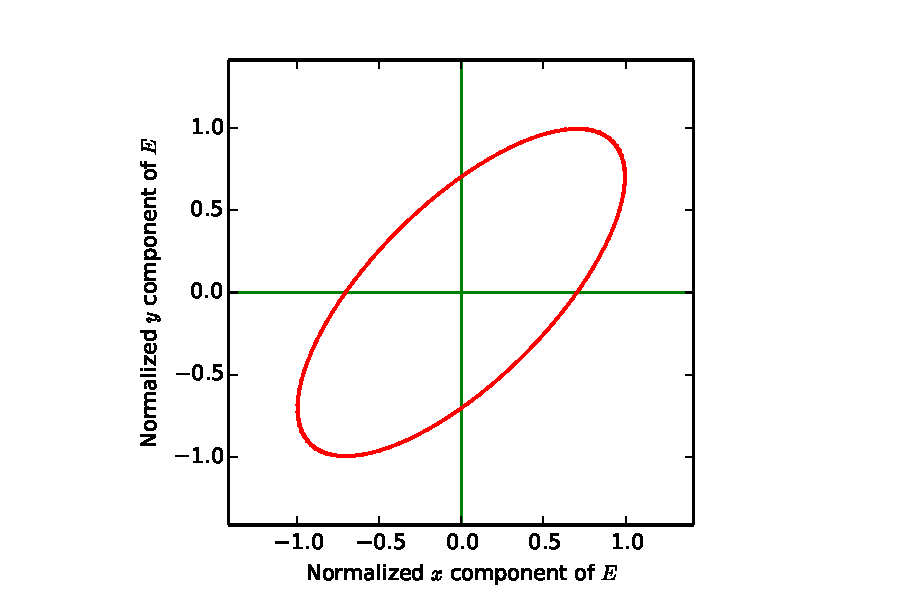
\includegraphics[width=1\linewidth]{ellipse_clean}
  %\caption{Elipse arbitraria que resulta cuando se observa la
   % variación temporal de un campo sobre el plano.}
  \caption{}
\label{fig:ellipse_clean}
\end{subfigure}\qquad
\begin{subfigure}{.45\textwidth}
  \centering
  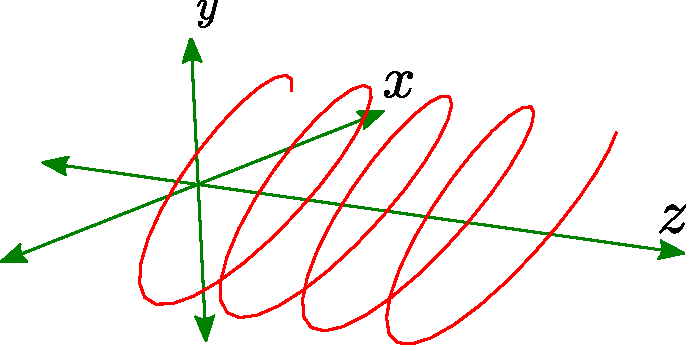
\includegraphics[width=.8\linewidth]{trayectory_clean}
 % \caption{Trayectoria helicodidal de la variación espacial de un
  %  campo óptico a lo largo de $z$.}
  \caption{}
  \label{fig:trayectory_clean}
\end{subfigure}
\caption[Distintas representaciones del campo eléctrico para ilustrar
la polarización]{Representaciones de la posición de un vector de campo
  eléctrico con polarización elíptica cuando (a) se analiza en un
  punto en el espacio, y (b) se  congela el tiempo.} 
\label{fig:general_field}
\end{figure} 

Desde el punto de vista matemático, la Fig.~\ref{fig:ellipse_clean} se describe por medio de la Eq.~\ref{eq:ellipse} que es la ecuación de una cónica y se puede obtener
a partir de las expresiones (\ref{eq:xcomp}) y (\ref{eq:ycomp}). 

Si $\delta = \delta_y-\delta_x$ y $z=0$,
entonces el campo se puede escribir como

\begin{align*}
E_x &= A_x\cos{ \left(\omega t \right)},\\
E_y &= A_y\cos{ \left(\omega t -\delta\right)}.
\end{align*}
Y se puede despejar los términos correspondientes al $\sin$ y $\cos$
 \begin{align*}
\cos{\omega t} &=\frac{E_x}{A_x},\\
\sin^2{\omega t} &= 1-\left(\frac{E_x}{A_x}\right)^2,\\
\sin{\omega t} &= \sqrt{1-\left(\frac{E_x}{A_x}\right)^2}.
\end{align*}
Por otra parte se tiene
\begin{equation}
  \label{eq:Ey-2}
E_y = A_y\left( \cos{\omega t}\cos{\delta}+\sin{\omega
    t}\sin{\delta}\right).  
\end{equation}
Reemplazando $\sin{\omega t} $ y $\cos{\omega t} $ en la expresión
(\ref{eq:Ey-2}) obtenemos
\begin{align}
E_y &= \frac{A_yE_x}{A_x}\cos{\delta} +
A_y\sqrt{1-\frac{E_x}{A_x}}\sin{\delta},\notag\\
\frac{E_y}{A_y} - \frac{E_x}{A_x}\cos{\delta}  &= 
\sqrt{1-\left(\frac{E_x}{A_x}\right)^2}\sin{\delta}.\label{eq:ellipse_nos}
\end{align}
Elevando al cuadrado la Eq.~(\ref{eq:ellipse_nos}) y organizando
términos, obtenemos la ecuación general de una elipse inscrita en un
rectángulo con lados $2A_x$, $2A_y$ 
\begin{equation}
\left(\frac{E_x}{A_x}\right)^2+\left(\frac{E_y}{A_y}\right)^2-2\frac{\cos{\delta}}{A_xA_y}E_xE_y
= \sin^2{\delta}.
\label{eq:ellipse}
\end{equation}
Se puede ahora plantear una rotación de un ángulo $\phi$ con respecto
al eje horizontal ($x$) sobre el sistema de coordenadas  como se
muestra en la Fig.~\ref{fig:ellipse} para que
el eje mayor de la elipse quede alineado con el eje
\textit{horizontal} del nuevo sistema. 
\begin{figure}[h!]
\centering
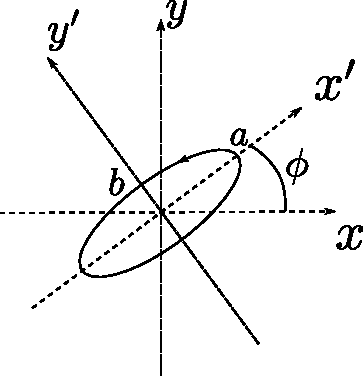
\includegraphics[scale = 1]{ellipse}
\caption[Rotación del sistema de coordenadas de la elipse de polarización]{Rotación del sistema de coordenadas un ángulo $\phi$.}
\label{fig:ellipse}
\end{figure}
Haciendo esto, se lleva la
Eq.~(\ref{eq:ellipse}) a la forma más conocida de la Eq.~(\ref{eq:new_ellipse})
\begin{equation}
\left(\frac{E_{x'}}{a}\right)^2+\left(\frac{E_{y'}}{b}\right)^2 = 1,
\label{eq:new_ellipse}
\end{equation}
dónde $a$ y $b$ son los semi ejes mayor y menor, y $E_{x'}$, $E_{y'}$
son las componentes del campo eléctrico en las direcciones $x'$,
$y'$. Los semiejes de la elipse están dados por las siguientes
expresiones \citepChGen{Yariv2002}:
\begin{align*}
a^2 = A_x\cos^2{\phi}+A_y^2\sin^2{\phi} +2A_xA_y \cos{\delta}\cos{\phi}\sin{\phi},\\
b^2 = A_x\sin^2{\phi}+A_y^2\cos^2{\phi} -2A_xA_y \cos{\delta}\cos{\phi}\sin{\phi}.
\end{align*}

La elipticidad se define como la razón entre el eje menor y el eje
mayor de la elipse $e=\pm\frac{b}{a}$ de tal forma que si el semi eje
menor es cero, la elipse se vuelve una linea y por tanto se dice que
la polarización es lineal en la dirección de $a$. Si por el contrario
los dos semi ejes tienen  la misma longitud, la ecuación de la elipse
se vuelve la de un círculo, y se dice que la polarización es
circular como en la Fig.~\ref{fig:circular_polarizations}(a). 
El signo de la elipticidad determina el sentido 
de giro de la hélice, si el signo es positivo la elipse es circular
izquierda como en la Fig.~\ref{fig:circular_polarizations}(b) y es
circular derecha 
cuando el signo es negativo (Fig.~\ref{fig:circular_polarizations}(c)). Cabe
anotar que el sentido de giro de la polarización es una convención
que varía según el autor, algunos autores como \citetChGen{Yariv2002} interpretan el sentido de giro como
si se congelara el tiempo y se siguiera la punta del vector
$\mathbf{E}$ desde el momento inicial en adelante. Sin embargo, otros
autores como \citetChGen{Hecht2001}
interpretan el sentido de giro como si en un punto fijo vieran girar
el vector $\mathbf{E}$ que les llega en la medida que pasa el tiempo. 
En este documento hemos decidido escoger la primera convención dado
que es la predominante en las referencias que tratan el análisis de
cristales líquidos como elementos que afectan la polarización. 
\begin{figure}[h!]
\centering
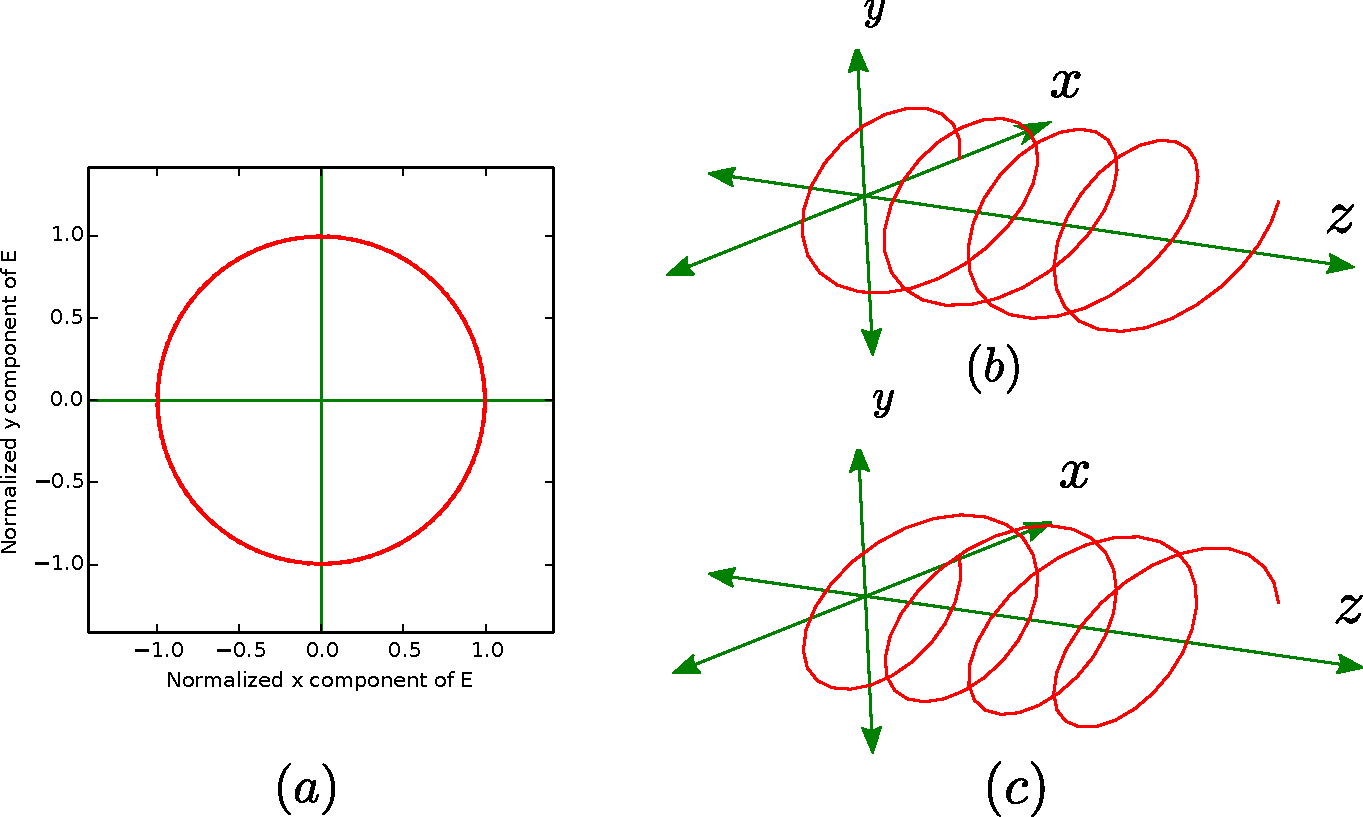
\includegraphics[scale=.5]{circular_polarizations}
\caption[Estados de polarización circular]{(a) Esquema de un estado de polarización circular en donde los semiejes
  de la elipse son iguales. La polarización circular izquierda (b) se da
cuando $e=\frac{b}{a}$ y la derecha (c) cuando  $e=-\frac{b}{a}$.}
\label{fig:circular_polarizations}
\end{figure}

Una ellipse de polarización arbitraria se puede expresar entonces
conociendo su elipticidad ($e$) y su ángulo de inclinación ($\phi$)
con respecto al eje horizontal. Estas dos características se pueden
parametrizar como dos ángulos que se dan en
términos de las amplitudes máximas del campo $A_x$, $A_y$
y el retardo entre componentes $\delta$. Por una parte, el ángulo de
inclinación se encuentra interpretando la Eq.~(\ref{eq:ellipse}) en
su forma bilineal de la forma
\begin{equation}
\begin{pmatrix}
E_x & E_y
\end{pmatrix}
\begin{pmatrix}
\frac{1}{A_x^2} & -\frac{\cos{\delta}}{A_xA_y}\\
 -\frac{\cos{\delta}}{A_xA_y} & \frac{1}{A_y^2} 
\end{pmatrix}
\begin{pmatrix}
E_x \\ E_y
\end{pmatrix}
=\sin^2{\delta},
\end{equation}
sacando factor común $\frac{1}{A_x^2} $ se obtiene
\begin{equation}
\begin{pmatrix}
E_x & E_y
\end{pmatrix}
\begin{pmatrix}
1 & -\frac{A_x\cos{\delta}}{A_y}\\
 -\frac{A_x\cos{\delta}}{A_y} & \frac{A_x/2}{A_y^2} 
\end{pmatrix}
\begin{pmatrix}
E_x \\ E_y
\end{pmatrix}
=A_x/2\sin^2{\delta},
\end{equation}
o en forma compacta
\begin{equation}
\begin{pmatrix}
E_x & E_y
\end{pmatrix}
\begin{pmatrix}
1 & a\\
 a & b 
\end{pmatrix}
\begin{pmatrix}
E_x \\ E_y
\end{pmatrix}
=c.
\end{equation}
%http://mpalffy.lci.kent.edu/Optics/Chapters/Ch7_Polarized%20Light.pdf

Una \href{http://es.wikipedia.org/wiki/Cu\%C3\%A1drica}{\textbf{cuádrica o superficie cuádrica}} es una  hipersuperficie D-dimensional
representada por una ecuación de segundo grado con 
coordenadas espaciales. Si estas coordenadas son $\{x_1,
x_2, ... x_D\}$, entonces la cuádrica típica en ese espacio se define
mediante la ecuación algebraica: 
\[ \sum_{i,j=1}^D Q_{i,j} x_i x_j + \sum_{i=1}^D P_i x_i + R = 0. \]
El caso particular en el cual solo hay dos dimensiones y los valores
$P_i$ son todos 0, es el de una elipse. En nuestro caso, tenemos en
notación matricial:
\[ \mathbf{E}^TQ\mathbf{E} + R= 0, \]
con
\[
Q=
\begin{pmatrix}
1 & a\\
 a & b 
\end{pmatrix}.
 \]
y $R=-c = -A_x/2\sin^2{\delta}$. Ahora, los autovalores de una elipse
representada por su forma matricial están asociados con la
dirección de sus ejes principales, y apuntan en la dirección de los
puntos máximos \citepChGen{Palffy1998}. Como nuestra incógnita es el ángulo
que determina la dirección de los puntos máximos, podemos escribir la
siguiente ecuación de autovalores para despejar $\phi$\footnote{
\url{http://en.wikipedia.org/wiki/Quadratic_form}}
\[\begin{pmatrix}
1 & a\\
 a & b 
\end{pmatrix} 
\begin{pmatrix}
\cos{\phi}\\
 \sin{\phi} 
\end{pmatrix} =
\lambda \begin{pmatrix}
\cos{\phi}\\
 \sin{\phi} 
\end{pmatrix} ,
\]
desarrollando, se obtienen las siguientes dos ecuaciones:
\begin{align*}
\cos{\phi} +a\sin{\phi} &= \lambda\cos{\phi},\\
a\cos{\phi} +b\sin{\phi} &= \lambda\sin{\phi}.
\end{align*}
Despejando $\lambda$ e igualando las ecuaciones se llega a una
expresión dependiente de un ángulo doble:
\[1+a\tan{\phi} = \frac{a}{\tan{\phi}}+b,\]
\[b-1= a\tan{\phi} -\frac{a}{\tan{\phi}},\]
\[ b-1=a\left(\frac{\tan^2{\phi} -1}{\tan{\phi}}\right),\]
\[\tan{2\phi} =\frac{2a}{b-1}.\]
Finalmente, reemplazando $a$, y $b$ se tiene el ángulo de inclinación
de la elipse:
\begin{equation*}
\phi = \frac{1}{2}\tan^{-1}{\left(\frac{2A_xA_y}{A_x^2-A_y^2}\cos{\delta}\right)}.
\end{equation*}
Siguiendo un esquema similar, aunque más tedioso se encuentra el
ángulo de elipticidad ($\theta = \tan^{-1}{e}$) en términos de la
función seno como:
\begin{equation*}
\theta = \frac{1}{2}\sin^{-1}{\left(\frac{2A_xA_y}{A_x^2+A_y^2}\sin{\delta}\right)}.
\end{equation*}
A la hora de despejar $\phi$ y $\theta$ reemplazando valores en la
primera ecuación usando un computador se aconseja reemplazar la función
$\tan^{-1}$ por la función atan2, que es popular en paquetes de
cálculos numéricos (como numpy) o lenguajes de programación como
Matlab, porque permite evitar las singularidades que ocurren cuando el argumento de la
función tangente inversa es $\pi/2$.

\subsection{El formalismo de Jones}

Se conoce como formalismo de Jones al uso de una representación
vectorial para describir campos ópticos coherentes y monocromáticos cuando es
importante la naturaleza vectorial de la luz y la polarización.  
En el esquema de Jones los campos ópticos con dos componentes ortogonales se
representan como un vector con elementos complejos conocido como
vector de Jones. Las dos componentes complejas del campo en la Eq.~(\ref{eq:complex_field}) se representan como elementos de un vector
columna conocido como vector de Jones:
 
\begin{equation}
\mathbf{J} =\begin{pmatrix} A_xe^{i\delta_x}\\A_ye^{i\delta_y}\end{pmatrix}.
\label{eq:jones_vector}
\end{equation}
Siendo un vector complejo, $\mathbf{J}$ no es una cantidad observable
en el espacio físico. Para obtener por ejemplo, la
componentente  $x$ del campo eléctrico se hace la operación $E_x(t) = \Re
\left[J_xe^{i\omega t}\right]$.
Para el estudio de la polarización conviene representar el vector de
Jones en su forma normalizada, es decir tal que cumpla la
condición, $$\mathbf{J}^{\dagger}\mathbf{J}=1,$$
dónde el símbolo $\dagger$ representa la transpuesta conjugada.
La normalización se logra parametrizando las amplitudes con el ángulo
del vector que forman, $$\tan{\psi}=\frac{\sin{\psi}}{\cos{\psi}}=\frac{A_y}{A_x},$$
de esta forma $A_y=\sin{\psi}$ y $A_x = \cos{\psi}$. Adicionalmente,
la fase de las componentes se acostumbra a escribir en su forma
relativa y con respecto a la componente $y$ como se muestra en la
expresión (\ref{eq:normalized_jones_vector}).

\begin{equation}
\mathbf{J(\psi,\delta)} =\begin{pmatrix} \cos{\psi}\\\sin{\psi}e^{i\delta}\end{pmatrix}.
\label{eq:normalized_jones_vector}
\end{equation}

\subsubsection{Algunos estados de polarización importantes}
Como se dijo antes, las polarizaciones lineales se obtienen cuando las
componentes están en fase, es decir que $\delta =
\delta_y-\delta_x=0$. Sin embargo, la condición también se cumple cuando las
diferencias de fase entre las componentes son múltiplos de $\pi$. 
A continuación se muestran seis estados de polarización conocidos
como los \textbf{estados degenerados de polarización}
\citepChGen{Collett2005} que son importantes tanto en la teoría de
polarización de Jones como en la de Stokes para la composición y
detección de estados de polarización elípticos.
Los primeros dos estados degenerados corresponden a las polarizaciónes
lineales ($\delta = n\pi$ ) horizontal y vertical que se dan cuando $\psi
= n\pi$ y $\psi = \frac{\pi}{2}(2n+1)$ respectivamente:
\begin{align*}
\mathbf{H} &=\begin{pmatrix}1\\0\end{pmatrix},& \mathbf{V} &=\begin{pmatrix}0\\1\end{pmatrix}.
\end{align*}
Luego, están los estados con polarización lineal a $45^{\circ}$ y
$-45^{\circ}$. El primero se da cuando las componentes $x$
y $y$ tienen la misma magnitud y dirección, es decir cuando
$\psi=\frac{\pi}{4}(4n+1)$. La polarización a  $-45^{\circ}$ se da cuando
$\psi=\frac{\pi}{4}(4n-1)$.
\begin{align*}
\mathbf{45^{\circ}}
&=\begin{pmatrix}\cos{\pi/4}\\\sin{\pi/4}\end{pmatrix}=\frac{1}{\sqrt{2}}
\begin{pmatrix}1\\1\end{pmatrix},&
\mathbf{-45^{\circ}} 
&=\begin{pmatrix}\cos{-\pi/4}\\\sin{-\pi/4}\end{pmatrix}=\frac{1}{\sqrt{2}}\begin{pmatrix}1\\-1\end{pmatrix}. 
\end{align*} 
Finalmente, se tienen los estados circulares que consisten en las
polarizaciones circular izquierda y circular derecha. Los estados de
polarozación circulares son tales que
ambas componentes tienen la misma magnitud que los de $\pm45^{\circ}$,
pero el retardo en fase entre ellas es de $\delta = \frac{\pi}{2}$:
\begin{align*}
\mathbf{CD}
&=\begin{pmatrix}\cos{\pi/4}\\\sin{\pi/4}e^{i\frac{\pi}{2}}\end{pmatrix}=\frac{1}{\sqrt{2}}
\begin{pmatrix}1\\i\end{pmatrix},&
\mathbf{CI} 
&=\begin{pmatrix}\cos{-\pi/4}\\\sin{-\pi/4}e^{i\frac{\pi}{2}}\end{pmatrix}=\frac{1}{\sqrt{2}}\begin{pmatrix}1\\-i\end{pmatrix}. 
\end{align*} 
Una característica interesante de los estados lineales y circulares es
que se pueden dar unos como combinación lineal de los otros:
\begin{align*}
\mathbf{CD} &= \frac{1}{\sqrt{2}}\left( \mathbf{H} -
  i\mathbf{V}\right),\\
\mathbf{CI} &= \frac{1}{\sqrt{2}}\left( \mathbf{H} +
  i\mathbf{V}\right),\\
\mathbf{H} &= \frac{1}{\sqrt{2}}\left( \mathbf{CD} +
  \mathbf{CI}\right),\\
\mathbf{V} &= \frac{i}{\sqrt{2}}\left( \mathbf{CD} -
  \mathbf{CI}\right).
\end{align*}
Los vectores de las tres parejas de estados que hemos visto hasta
ahora son bases ortonormales. Esto quiere decir que fuera de estar
normalizados, %son linealmente independientes entre sí, 
si calculamos el producto escalar entre elementos de una misma pareja
obtenemos un valor de 0,
% \begin{equation*}
% \begin{pmatrix}1&0\end{pmatrix}\begin{pmatrix}0\\1\end{pmatrix}=
% \left(\frac{1}{\sqrt{2}}\begin{pmatrix}1&1\end{pmatrix}\right)\left(\frac{1}{\sqrt{2}}\begin{pmatrix}1\\-1\end{pmatrix}\right)  = \left(\frac{1}{\sqrt{2}}
% \begin{pmatrix}1&i\end{pmatrix}\right)\left(\frac{1}{\sqrt{2}}\begin{pmatrix}1\\-i\end{pmatrix}\right)
% = 0.
% \end{equation*}
\begin{equation*}
\mathbf{H^{\dagger}V} = \mathbf{45^{\circ\dagger}-45^{\circ}} =
\mathbf{CD^{\dagger}CI = 0.}   
\end{equation*}
Estos estados se han mencionado porque sirven como base para el espacio
de posibles estados de polarización y serán usados en la sección
\ref{sec:ChGV_med_mod_amp} para producir curvas de modulación de
amplitud que alimentan un modelo de calibración de moduladores capaz
de predecir la modulación para otros estados. 

\subsubsection{Elementos ópticos como operadores en la representación
  de Jones}

Así como en el álgebra lineal se usan matrices para transformar
vectores, en el formalismo de Jones existen operadores que se
representan como matrices 2x2 y que tienen la cualidad de
transformar los campos. Estos operadores se conocen como matrices de
Jones y deben cumplir algunas
propiedades generales \citepChGen{Yariv2002} que se listan a continuación:

\begin{enumerate}
\item La dirección de propagación de un campo determina las
  componentes de la matriz que representa al elemento polarizador. Si
  la incidencia es desde la izquierda $(z=0)$ definimos la matriz $M$ como aquella
  que transforma el vector de entrada en el de salida,
  \begin{equation}
    \begin{pmatrix}
      V_x^{out}\\V_y^{out}
    \end{pmatrix}
    =
    \begin{pmatrix}
      M_{11}&M_{12}\\M_{21} & M_{22}
    \end{pmatrix}
    \begin{pmatrix}
      V_x^{in}\\V_y^{in}
    \end{pmatrix},
    \label{eq:right_propagation}
  \end{equation}
si el vector de entrada ingresa desde la derecha entonces
definiremos una matriz distinta $N$ para representar la transformación:
  \begin{equation*}
    \begin{pmatrix}
      V_x^{out}\\V_y^{out}
    \end{pmatrix}
    =
    \begin{pmatrix}
      N_{11}&N_{12}\\N_{21} & N_{22}
    \end{pmatrix}
    \begin{pmatrix}
      V_x^{in}\\V_y^{in}
    \end{pmatrix}.
  \end{equation*}

Para que se cumpla el principio de simetría temporal, se debe cumplir
que $NM=1$. Si se \textit{rebobina} la propagación en la expresión
(\ref{eq:right_propagation}) el haz de salida 
debería seguir el mismo camino que recorrió a la entrada, y ser
afectado por la matriz $N$ de tal forma que vuelva a la forma que
tenía en un principio,
 \begin{align*}
    \begin{pmatrix}
      V_x^{in}\\V_y^{in}
    \end{pmatrix}
    &=
    \begin{pmatrix}
      N_{11}&N_{12}\\N_{21} & N_{22}
    \end{pmatrix}
    \begin{pmatrix}
      V_x^{out}\\V_y^{out}
    \end{pmatrix},\\
    &=
    \begin{pmatrix}
      N_{11}&N_{12}\\N_{21} & N_{22}
    \end{pmatrix}
    \begin{pmatrix}
      M_{11}&M_{12}\\M_{21} & M_{22}
    \end{pmatrix}
    \begin{pmatrix}
      V_x^{in}\\V_y^{in}
    \end{pmatrix}.\\
  \end{align*}
  Conociendo que las matrices están asociadas a un mismo elemento se
  debe cumplir que $N$ sea la transpuesta de $M$
  \begin{align*}
    N_{11}&=M_{11},&    N_{12}&=M_{21},&     N_{21}&=M_{12}, &     N_{22}&=M_{22}.
  \end{align*}
Esta relación es importante para analizar sistemas en los cuales la
luz debe pasar dos veces por el LC en sentidos opuestos, caso especial
es el de los SLM's de reflexión en los cuales hay una
superficie especular de un lado.

\item Tanto la matriz $M$ como la $N$ son operadores unitarios,
  \begin{align*}
    M^{\dagger} M &= 1,& N^{\dagger}N &=1.
  \end{align*}
Dónde el símbolo $\dagger$ indica que se saca el conjugado hermítico
de $M$,
\begin{equation*}
M^{-1}=M^{\dagger}=
  \begin{pmatrix}
      M_{11}^*&M_{21}^*\\M_{12}^* & M_{22}^*
    \end{pmatrix}.
\end{equation*}
\item Las matrices de Jones son también unimodulares es decir
\begin{equation}det(M) = det(M^{\dagger})  = M_{11}M_{22}-M_{12}M_{21} = 1.\label{eq:unimodular}\end{equation} 
Si asumimos que $M^{-1}$ es
\begin{equation*}
  M^{-1}=
  \begin{pmatrix}
    M_{22}&-M_{12}\\-M_{21}&M_{11}
  \end{pmatrix},
\end{equation*}
se ve que cumple con la relación $M^{-1}M = 1$:
\begin{align*}
    \begin{pmatrix}
    M_{22}&-M_{12}\\-M_{21}&M_{11}
  \end{pmatrix}
\begin{pmatrix}
      M_{11}&M_{12}\\M_{21} & M_{22}
    \end{pmatrix}
&=
    \begin{pmatrix}
 M_{22}M_{11}-M_{12}M_{21}     & M_{22}M_{12}-M_{12}M_{22}\\
-M_{11}M_{21}+M_{11}M_{21}    & -M_{12}M_{21} + M_{11}M_{22} 
    \end{pmatrix},\\
&=
\begin{pmatrix}
  1 &0\\0&1
\end{pmatrix}.
\end{align*}
Con esto, se puede simplificar la forma de una matriz de Jones a
partir de las siguientes relaciones,
\begin{align*}
  M_{21} &= - M_{12}^*, & M_{22} = M_{11}^*,
\end{align*}
obteniendo una forma de la matriz que depende de sólo dos números
complejos:
\begin{align}
  M&=
  \begin{pmatrix}
    A & B \\-B^* & A^*
  \end{pmatrix}\\
&=
  \begin{pmatrix}
    X+iY & Z+iW \\-Z+iW& X-iY
  \end{pmatrix}
\label{eq:general_jones_matrix}
\end{align}

Tener la matriz en esta forma facilita encontrar los parámetros de elementos
ópticos desconocidos como un SLM porque reduce el número de incógnitas.

\end{enumerate}

Los operadores que se verán a
continuación hacen referencia a dos tipos de elementos ópticos que se
utilizan en el laboratorio para modificar los estados de polarización
de una onda, estos son, polarizadores y retardadores. Los polarizadores
son elementos que afectan únicamente la amplitud y los
retardadores introducen retardos de la fase entre las componentes del campo.
Por una parte, los polarizadores horizontales son elementos que sólo
dejan pasar la componente $x$ del campo, y se representan con la
matriz de la Eq.~(\ref{eq:Px_matrix}),
\begin{equation}
P_x = \begin{pmatrix}1 &0\\0&0\end{pmatrix}.
\label{eq:Px_matrix}
\end{equation}
Si llega cualquier campo al polarizador horizontal este dejará pasar
sólo la componente $x$ tal y
como se muestra en la Fig.~\ref{fig:linear_polarizer}. 
\begin{figure}[h!]
\centering
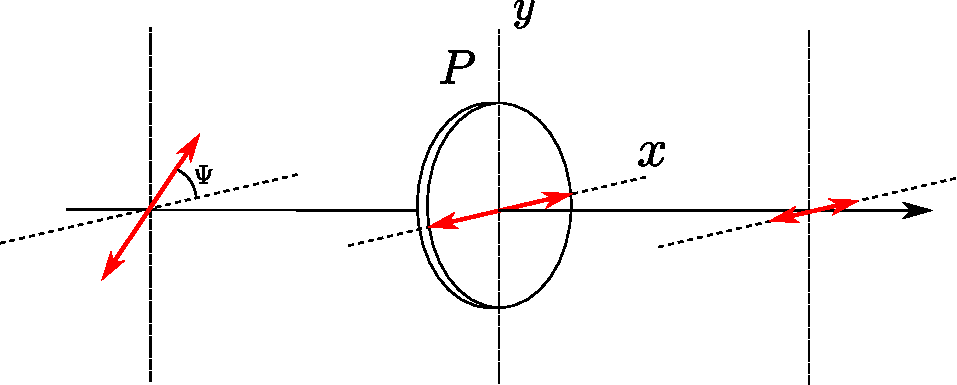
\includegraphics[scale = .7]{linear_polarizer}
\caption{Propagación de un estado de polarización lineal a través de
  un polarizador horizontal.}
\label{fig:linear_polarizer}
\end{figure}
La  operación vectorial correspondiente a este fenómeno se da como la
multiplicación entre la matriz del polarizador y el vector de Jones
que representa al campo, en este caso un campo con polarización lineal
a $45^{\circ}$
\begin{equation*}
\frac{1}{\sqrt{2}}
\begin{pmatrix}
1\\0
\end{pmatrix}
=
\begin{pmatrix}
1 &0\\0&0
\end{pmatrix}
\frac{1}{\sqrt{2}}
\begin{pmatrix}
1 \\1
\end{pmatrix}.
\end{equation*}
Los polarizadores que no están orientados con el eje $x$ se pueden
obtener a partir de la matriz de $P_x$ por medio de la siguiente
operación de rotación, 
\begin{align*}
P_{\theta}&=R^T(\theta)P_xR(\theta)\\
P_{\theta}
&=
\begin{pmatrix}
  \cos{\theta} &-\sin{\theta}\\\sin{\theta}&\cos{\theta}
\end{pmatrix},
\begin{pmatrix}
1 & 0 \\0& 0
\end{pmatrix}
\begin{pmatrix}
  \cos{\theta} &\sin{\theta}\\-\sin{\theta}&\cos{\theta}
\end{pmatrix}.
\end{align*}
En adelante se seguirá usando este método para representar la matriz de cualquier
elemento óptico rotado.
Reemplazando $\theta = \frac{\pi}{2}$ y $\theta = \frac{\pi}{4}$
obtenemos las matrices $P_y$ y $P_{45^{\circ}}$ correspondientes al
polarizador alineado con $y$ y al que está inclinado $45^{\circ}$:
\begin{align*}
P_{y}
&=
\begin{pmatrix}
  \cos{\frac{\pi}{2}} &-\sin{\frac{\pi}{2}}\\\sin{\frac{\pi}{2}}&\cos{\frac{\pi}{2}}
\end{pmatrix}
\begin{pmatrix}
1 & 0 \\0& 0
\end{pmatrix}
\begin{pmatrix}
  \cos{\frac{\pi}{2}} &\sin{\frac{\pi}{2}}\\-\sin{\frac{\pi}{2}}&\cos{\frac{\pi}{2}}
\end{pmatrix},\\
&=
\begin{pmatrix}
  0&-1\\1&0
\end{pmatrix}
\begin{pmatrix}
1 & 0 \\0& 0
\end{pmatrix}
\begin{pmatrix}
0 &1\\-1&0
\end{pmatrix},\\
&=
\begin{pmatrix}
0 &0\\0&1
\end{pmatrix}.\\
\end{align*}
\begin{align*}
P_{45^{\circ}}
&=
\begin{pmatrix}
  \cos{\frac{\pi}{4}} &-\sin{\frac{\pi}{4}}\\\sin{\frac{\pi}{4}}&\cos{\frac{\pi}{4}}
\end{pmatrix}
\begin{pmatrix}
1 & 0 \\0& 0
\end{pmatrix}
\begin{pmatrix}
  \cos{\frac{\pi}{4}} &\sin{\frac{\pi}{4}}\\-\sin{\frac{\pi}{4}}&\cos{\frac{\pi}{4}}
\end{pmatrix},\\
&=
\frac{1}{\sqrt{2}}
\begin{pmatrix}
  1&-1\\1&1
\end{pmatrix}
\begin{pmatrix}
1 & 0 \\0& 0
\end{pmatrix}
\frac{1}{\sqrt{2}}
\begin{pmatrix}
1 &1\\-1&1
\end{pmatrix},\\
&=
\frac{1}{2}
\begin{pmatrix}
1 &1\\1&1
\end{pmatrix}.\\
\end{align*}
Por otra parte, los retardadores ópticos modifican tanto la amplitud
como la fase de las componentes del campo y sus elementos son
complejos. La matriz general para un retardador óptico con desfase
$\beta $ y orientación del eje rápido con el eje
$x$ es,
\begin{equation}
WP = 
\begin{pmatrix}
e^{i\beta/2} & 0 \\0&e^{-i\beta/2}  
\end{pmatrix}
\label{eq:retarder}
\end{equation}
Los retardadores ópticos se construyen a partir de materiales
birrefringentes donde el retardo de fase $\beta$ de una componente con respecto a otra es
proporcional a la diferencia de índices de refracción, y a la
profundidad $d$ del medio birrefringente,
$$\beta= \frac{\pi}{2}d\left(n_e-n_o\right).$$ 
Dónde el índice de refracción extraordinario corresponde al eje rápido
del medio, y el extraordinario al eje lento \citepChGen{Yariv2002}. Si multiplicamos la
Eq.~(\ref{eq:retarder}) por $e^{-i\beta/2} $ 
obtenemos la forma no normalizada que es muy común en los libros de
texto porque en ella se hace evidente que la componente $E_y$ del
campo sufre un retardo en fase de $\beta$ con respecto a $E_x$,  
\begin{equation*}
W = 
\begin{pmatrix}
1& 0 \\0&e^{-i\beta}  
\end{pmatrix}.
\label{eq:retarder_2}
\end{equation*}
Los retardadores más usados en el laboratorio son aquellos que
introducen retardos de cuarto de onda:
\begin{equation*}
QWP = \begin{pmatrix} e^{i\frac{\pi}{4}}  &0\\0&e^{-i\frac{\pi}{4}}\end{pmatrix}
=  \begin{pmatrix} 1 &0\\0&e^{-i\frac{\pi}{2}}\end{pmatrix}
=  \begin{pmatrix} 1 &0\\0&-i\end{pmatrix}.
\end{equation*}
y retardos de
media onda:
\begin{equation*}
HWP = \begin{pmatrix} e^{i\frac{\pi}{2}}
  &0\\0&e^{-i\frac{\pi}{2}}\end{pmatrix} =  \begin{pmatrix} 1
  &0\\0&e^{-i\frac{\pi}{2}}\end{pmatrix} =  \begin{pmatrix} 1 &0\\0&-1\end{pmatrix},
\end{equation*}
Los de cuarto de onda permiten obtener polarizaciones
circulares o elípticas a partir de polarizaciones lineales. La Fig.~\ref{fig:qwp_retarder} muestra cómo conseguir un campo con
polarización circular derecha a partir de polarización lineal y un 
retardador $QWP$.
\begin{figure}[h!]
\centering
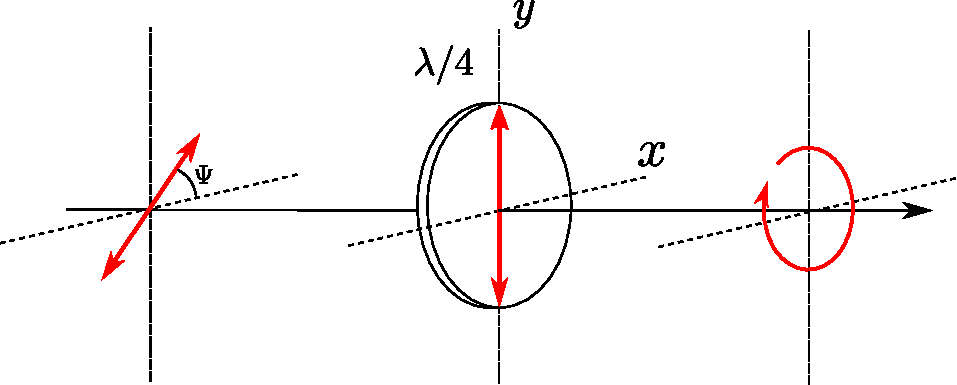
\includegraphics[scale=.7]{qwp_retarder}
\caption[Generación de estados de polarización circulares]{Propagación de un estado de polarización lineal a
  $45^{\circ}$ a través de una placa de retardo de cuarto de onda
  vertical que genera un estado de polarización circular derecho. Las
placas de cuarto de onda introducen un retardo de fase de
$\frac{\pi}{2}$ radianes.}
\label{fig:qwp_retarder}
\end{figure}
La operación correspondiente en el formalismo de Jones es,
\begin{align*}
\mathbf{CD} &=
R^{T}\left(\frac{\pi}{2}\right)\left(QWP\right)R\left(\frac{\pi}{2}\right)\mathbf{45}^{\circ},\\ 
  \frac{1}{\sqrt{2}}
\begin{pmatrix}
1\\i
\end{pmatrix}&=
\begin{pmatrix}
  0 &-1\\1&0
\end{pmatrix}
\begin{pmatrix} e^{i\frac{\pi}{4}}  &0\\0&e^{-i\frac{\pi}{4}} \end{pmatrix}
\begin{pmatrix}
  0&1\\-1&0
\end{pmatrix}
 \frac{1}{\sqrt{2}}
\begin{pmatrix}
1\\ 1
\end{pmatrix},
\\
&=
\begin{pmatrix}
e^{-i\frac{\pi}{4}}  & 0 \\0 & e^{i\frac{\pi}{4}} 
\end{pmatrix}
  \frac{1}{\sqrt{2}}
\begin{pmatrix}
1\\ 1
\end{pmatrix},\\
&=
\begin{pmatrix}
1  & 0 \\0 & i
\end{pmatrix}
  \frac{1}{\sqrt{2}}
\begin{pmatrix}
1\\ 1
\end{pmatrix}.
\end{align*}
En cambio, los retardadores de media onda permiten rotar el estado de
polarización sin afectar la intensidad a la salida. En la
figura \ref{fig:hwp_retarder} se muestra cómo una placa de media onda
orientada a $45^{\circ}$ puede rotar un estado de polarización lineal
horizontal a uno vertical. 
\begin{figure}[h!]
\centering
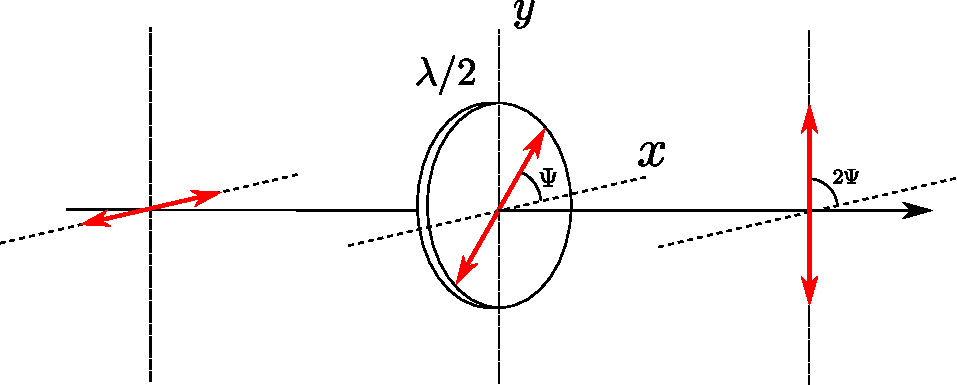
\includegraphics[scale=.7]{HWP_retarder}
\caption[Generación de estados de polarización lineales]{Propagación de un estado de polarización lineal horizontal a través de una placa de retardo de media onda
  vertical a $45^{\circ}$ que genera un estado de polarización lineal vertical. Las
placas de media onda introducen un retardo de fase de
$\pi$ radianes.}
\label{fig:hwp_retarder}
\end{figure}
Como en los casos anteriores, se puede representar la rotación de la
polarización usando el formalismo de Jones:
\begin{align*}
\mathbf{V} &=
R^{T}\left(\frac{\pi}{4}\right)\left(HWP\right)R\left(\frac{\pi}{4}\right)\mathbf{H},\\ 
\begin{pmatrix}
0\\1
\end{pmatrix}&=
 \frac{1}{\sqrt{2}}
\begin{pmatrix}
  1 &-1\\1&1
\end{pmatrix}
\begin{pmatrix} 1
  &0\\0&-1 \end{pmatrix}
 \frac{1}{\sqrt{2}}
\begin{pmatrix}
1&1\\-1&1
\end{pmatrix}
\begin{pmatrix}
1\\ 0
\end{pmatrix},
\\
&=
\begin{pmatrix}
0  & 1 \\1 & 0
\end{pmatrix}
\begin{pmatrix}
1\\ 0
\end{pmatrix},\\&=
\begin{pmatrix}
0\\1
\end{pmatrix}.
\end{align*}
Combinando rotadores ópticos (HWP) y retardadores de cuarto de onda
(QWP), 
podemos generar polarizaciones elípticas con cualquier inclinación y
elipticidad. Así como estos elementos pueden ser modelados por una
matriz, el SLM, que es también un elemento birrefringente que
transforma los estados de polarización puede ser modelado con matrices
de Jones que cumplen las mismas propiedades generales. 
% Esto será de utilidad más adelante pues los autovectores
% de las matrices de Jones indican los estados de polarización para los
% cuales el sistema es transparente, es decir, no se modifica el vector
% tras la operación de la matriz,
% \[\mathbf{M}J_{\lambda} = \lambda J_{\lambda}.\]
% Cuando se desea modulación de sólo fase en un SLM lo que se busca es
% precisamente que no se modifique la polarización y por ende la
% amplitud. El problema de calibrar moduladores se reduce a encontrar la
% matriz que define el LC y extraer sus autoestados tal y como dicen
% Pezzanitti y Davis en \citepChGen{Pezzaniti1993,Davis1998,Davis2003}.
En la sección que sigue se construirá un modelo para describir el
comportamiento de un cristal líquido enroscado (TN-LCD) en términos de
matrices de Jones.

\subsection{Propiedades ópticas de los cristales líquidos nemáticos enroscados (TN-LCD)}
\label{sec:Propiedades_opticas_de_TNLCD}
Los cristales líquidos del tipo TN-LCD son medios ópticos inhomogeneos
y anisotrópicos que localmente actúan como si fueran cristales
birrefringentes uniaxiales con su eje óptico orientado en la dirección
preferente de las moléculas. Como se mencionó en la sección
\ref{sec:LC-clasification} la anisotropía se debe a la forma obloide
de las moléculas del cristal, y en el caso de los TN la inhomogeneidad
viene dada por la orientación preferencial de las moléculas que es
función de su posición. Las propiedades ópticas se estudian suponiendo
que el material se puede representar como láminas delgadas perpendiculares a la
dirección de propagación, cada una de ellas actuando como si fuera un
cristal birrefringente uniaxial con su eje óptico rotado respecto al eje $x$ un ángulo
$\psi$ como se ilustra en la Fig.~\ref{fig:tn-lcd_sticks}.  
\begin{figure}[h!]
\centering
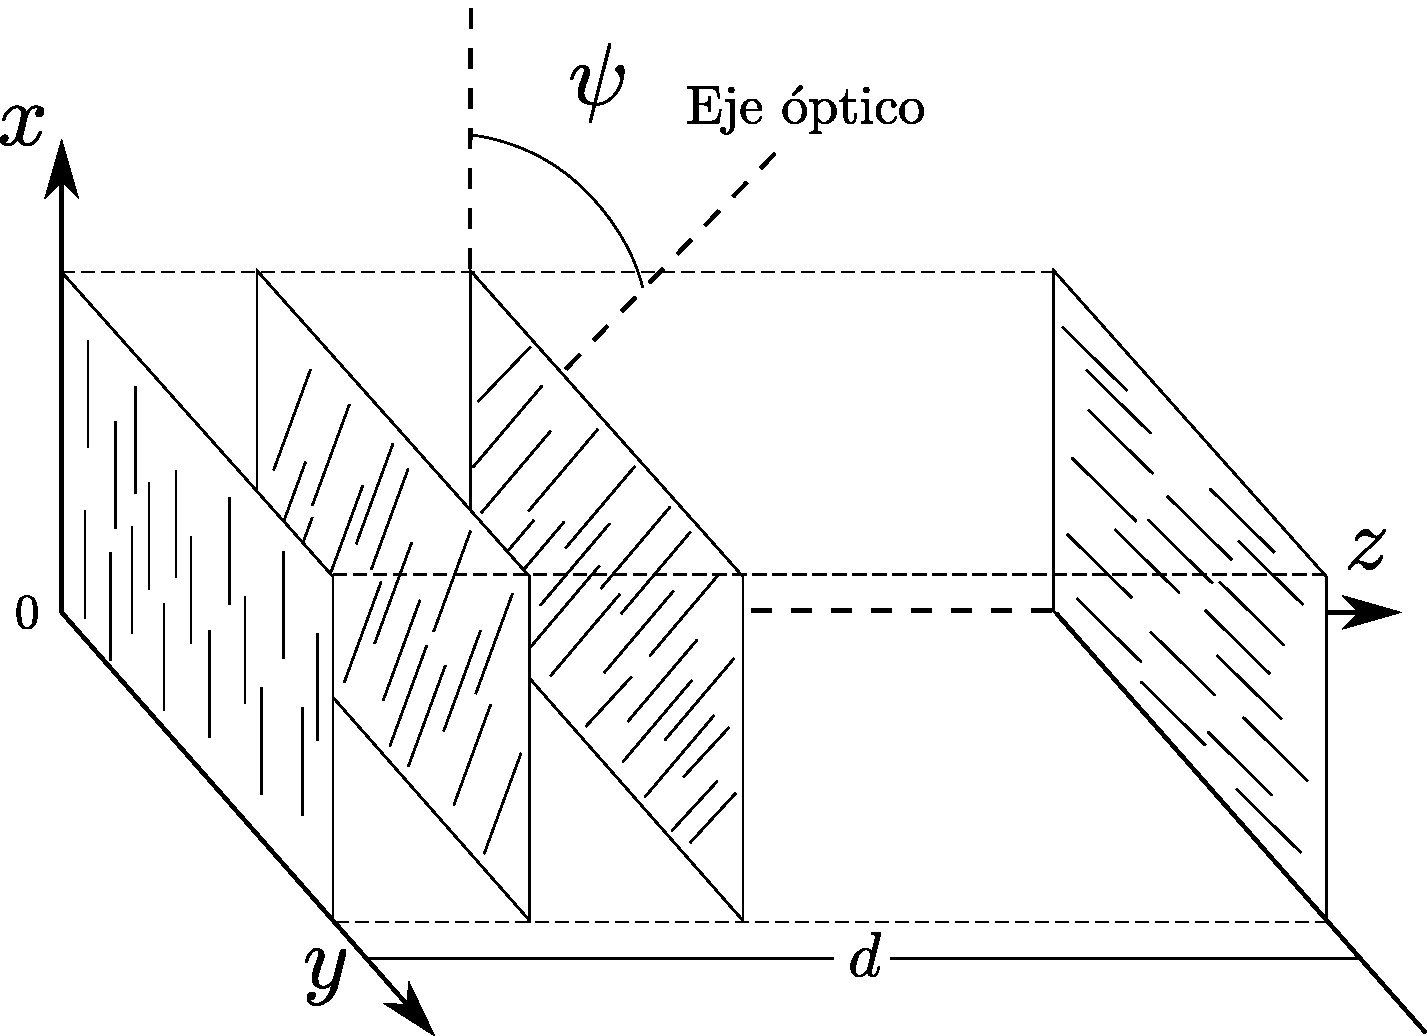
\includegraphics[scale = .3]{TN-LCD_sticks}
\caption[Propagación de la luz en un TN-LC]{Propagación de la luz en
  un cristal líquido del tipo Twisted 
  Nematic. En este diagrama el ángulo de entorchado es de $90^{\circ}$.}
\label{fig:tn-lcd_sticks}
\end{figure}
La rotación de cada \textit{lámina} de
moléculas se asume proporcional a la distancia desde la superficie de
entra da del LCD \citepChGen{Yariv2002},
\begin{equation}
  \label{eq:twist_angle}
\psi(z)  =\alpha z.  
\end{equation}
Aquí la constante $\alpha$
se conoce como coeficiente de torsión, y el ángulo a la salida viene
dado por $$\phi \equiv \psi(d)=\alpha d.$$ Si se divide el cristal en
$N$ láminas, cada una tendrá un grosor $d/N$ y estará orientada en los ángulos
$\rho,2\rho,3\rho,\dots\left(N-1\right)\rho,N\rho$ con
$\rho=\phi/N$. Si cada lámina representa un cristal birrefringente, ésta tendrá una
birrefringencia asociada a su grosor dada por $$\beta_N = \frac{\pi
  d}{2N}\left(n_e-n_o\right).$$
La matriz de Jones general para el conjunto de todas las láminas se
encuentra como la multiplicación de cada una como se muestra a
continuación:
\[ M= W_NW_{N-1}\cdots W_3W_2W_1=\prod_{m=1}^NW_m = \prod_{m=1}^NR(m\rho)^TW_0R(m\rho), \]
dónde $R$ es la matriz de rotación, $W_m$ es la matriz de Jones para
el retardador $m$ rotada, y $W_0$ es aquella lámina en donde el eje rápido está
orientado con el eje $x$,
\begin{equation*}
W_0 =
\begin{pmatrix}
  e^{i\beta/2N} &0 \\ 0 & e^{-i\beta/2N} 
\end{pmatrix}.
\end{equation*}
Las matrices de rotación cumplen la siguiente regla:
\begin{align*}
R^T(\psi_m)R^T(\psi_{m-1}) &= R^T\left(\psi_m+\psi_{m-1}\right),\\
&=
\begin{pmatrix}
  \cos{\psi_m}&  -\sin{\psi_m}\\  \sin{\psi_m}&  \cos{\psi_m}
\end{pmatrix}
\begin{pmatrix}
  \cos{\psi_{m-1}}&  -\sin{\psi_{m-1}}\\  \sin{\psi_{m-1}}&  \cos{\psi_{m-1}}
\end{pmatrix},\\
&=
\begin{pmatrix}
  \cos{\psi_m}\cos{\psi_{m-1}}-\sin{\psi_m}\sin{\psi_{m-1}}&  
-(\cos{\psi_m}\sin{\psi_{m-1}}+\sin{\psi_m} \cos{\psi_{m-1}})\\
  \sin{\psi_m} \cos{\psi_{m-1}}+\cos{\psi_m}\sin{\psi_{m-1}}& 
 -\sin{\psi_m}\sin{\psi_{m-1}}+\cos{\psi_m}\cos{\psi_{m-1}}
\end{pmatrix},  \\
&=\begin{pmatrix}
  \cos{\left(\psi_m+\psi_{m-1}\right)}&  -\sin{\left(\psi_m+\psi_{m-1}\right)}\\
  \sin{\left(\psi_m+\psi_{m-1}\right)}&  \cos{\left(\psi_m+\psi_{m-1}\right)} 
\end{pmatrix}.
\end{align*}
Usando esta propiedad de las matrices de rotación, se puede seguir el
siguiente razonamiento, si $N=1$ entonces,
\begin{equation*}
  M = R^T(\rho)W_0R(\rho).
\end{equation*}
Si en cambio $N=2$ se tiene
\begin{align*}
  M &= R^T(2\rho)W_0R(2\rho)R^T(\rho)W_0R(\rho),\\
      &=R^T(2\rho)W_0R(\rho)R(\rho)R^T(\rho)W_0R(\rho).
\end{align*}
Como $R(\rho)R^T(\rho)=\mathds{1}$ entonces,
\begin{align*}
 M &= R^T(2\rho)W_0R(\rho)W_0R(\rho),\\
     &=R^T(2\rho)\left[W_0R(\rho)\right]^2.
\end{align*}
Y para $N=3$:
\begin{align*}
  M &= R^T(3\rho)W_0R(3\rho)R^T(2\rho)W_0R(2\rho)R^T(\rho)W_0R(\rho),\\
      &=R^T(3\rho)W_0R(3\rho)R^T(2\rho)\left[W_0R(\rho)\right]^2,\\
      &=R^T(3\rho)W_0R(\rho)R(2\rho)R^T(2\rho)\left[W_0R(\rho)\right]^2,\\
      &=R^T(3\rho)W_0R(\rho)\left[W_0R(\rho)\right]^2,\\
      &=R^T(3\rho)\left[W_0R(\rho)\right]^3.
\end{align*}
Ahora, para una cantidad arbitraria $m$:
\begin{align*}
  M &= R^T(m\rho)W_0R(m\rho)R^T((m-1)\rho)\left[W_0R(\rho)\right]^{m-1},\\
      &=R^T(m\rho)W_0R(\rho)R((m-1)\rho)R^T((m-1)\rho)\left[W_0R(\rho)\right]^{m-1},\\  
      &=R^T(m\rho)W_0R(\rho)\left[W_0R(\rho)\right]^{m-1},\\
      &=R^T(m\rho)\left[W_0R(m\rho)\right]^{m}.
\end{align*}
Y así se obtiene la matriz general del TN-LCD según \citetChGen{Yariv2002} en
términos de dos matrices, una que cambia el estado de polarización y
otra que simplemente lo rota
\begin{align}
M&=R^T\left( \phi\right)
\left[W_0R\left(\frac{\phi}{N}\right)\right]^N,\\
&=R^T\left( \phi\right)
\begin{pmatrix}
  \cos{\frac{\phi}{N}e^{i\beta/N}} &  \sin{\frac{\phi}{N}e^{i\beta/N}}\\
  -\sin{\frac{\phi}{N}e^{-i\beta/N}} &  \cos{\frac{\phi}{N}e^{-i\beta/N}}  
\end{pmatrix}^N.
\label{eq:general_lcd_matrix}
\end{align}
La Eq.~(\ref{eq:general_lcd_matrix}) puede ser simplificada aún
mas como muestran \citetChGen{Yeh1999} si se usa la identidad de Chebyshev
para matrices unimodulares  
\begin{equation}
  \begin{pmatrix}
    A & B \\ C & D
  \end{pmatrix}^m
=
\begin{pmatrix}
  \frac{A\sin{ (mZ) }-\sin(m-1)Z }{\sin{Z} }
  &\frac{B\sin{(mZ)}}{\sin{Z}}\\
\frac{C\sin{(mZ)}}{\sin{Z}}&   \frac{D\sin{ (mZ) }-\sin(m-1)Z }{\sin{Z} }
\end{pmatrix},
  \label{eq:chebyshev}
\end{equation}
con \[Z = \cos^{-1}{\left[\frac{1}{2}(A+D)\right]}.\]
Si se saca el límite cuando $(N\rightarrow \infty)$
\citetChGen{Saleh1990} muestran que se puede obtener la
siguiente matriz,
\begin{equation}
  \label{eq:TN-LCD_Jones_Matrix}
  M=
  \begin{pmatrix}
    \cos{\phi} & -\sin{\phi}\\\sin{\phi}&\cos{\phi}
  \end{pmatrix}
  \begin{pmatrix}
    \cos{\gamma}+i\beta\frac{\sin{\gamma}}{\gamma} & \phi\frac{\sin{\gamma}}{\gamma}\\
-\phi\frac{\sin{\gamma}}{\gamma}   & \cos{\gamma}-i\beta\frac{\sin{\gamma}}{\gamma}
  \end{pmatrix},
\end{equation} 
dónde
\[\gamma=\sqrt{\phi^2+\beta^2}.\]

Ahora, la matriz de la Eq.~(\ref{eq:TN-LCD_Jones_Matrix})  es la
matriz que todos los autores referenciados en el
estudio del estado del arte usan, y a partir de la cual se basan
para caracterizar moduladores. La matriz que representa un
SLM  tal como se estudió en esta sección es la forma más
simple de representar un cristal líquido del tipo twisted nematic y se
conoce como el modelo de \citetChGen{Saleh1990}. Este modelo
parte de asumir las siguientes aproximaciones:

\begin{itemize}
\item El TN-LCD se comporta como una sucesión de  láminas
  retardadoras en las cuales la orientación del vector director varía
  gradualmente desde un ángulo a la entrada hasta un ángulo a la
  salida y formando un ángulo de rotación conocido como twist angle. 
\item El ángulo de rotación (twist angle) es una función lineal
  proporcional a la profundidad en el cristal tal y como se expresa en
  la Eq.~(\ref{eq:twist_angle}).
\item El ángulo de inclinación (tilt angle) se produce cuando se
  introduce un campo eléctrico que hace rotar las moléculas para
  alinearlas en su dirección. Éste ángulo se asume constante a lo
  largo del cristal para un voltaje específico. Si la birrefringencia
  es proporcional al ángulo de inclinación, entonces al variar el
  voltaje ésta variará linealmente con respecto al voltaje.
\end{itemize}

En modelos posteriores como los de \citetChGen{Coy1996} y
\citetChGen{Marquez2000} se construyen matrices para el LCD que
corrigen comportamientos no lineales no previstos por  Lu y Saleh. El
principal factor a corregir en un LCD es la tendencia de las moléculas
cercanas a las paredes del cristal a conservar la dirección de pulido
de los vidrios que las contienen como se ilustra en la Fig.~\ref{fig:lcd_models}.
\begin{figure}[h!]
\centering
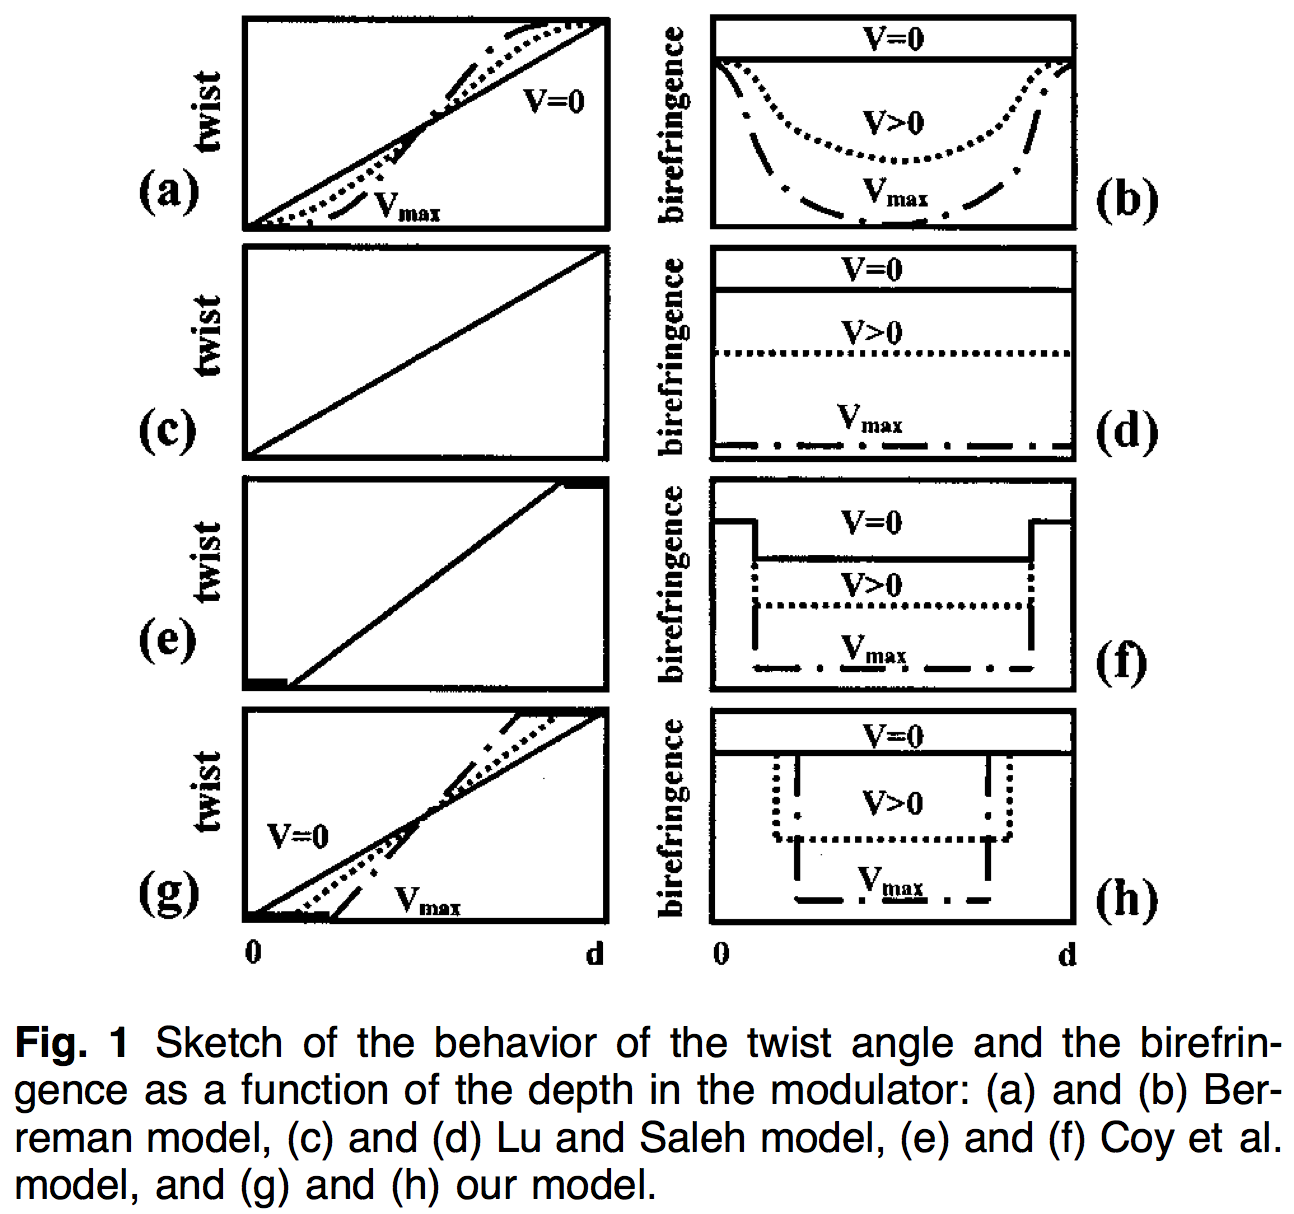
\includegraphics[scale=.5]{lcd_models}
\caption[Modelos de TN-LCD]{Modelos de TN-LCD tomado de \citetChGen{Marquez2000}.}
\label{fig:lcd_models}
\end{figure}
 Este efecto hace que el ángulo de
rotación no sea una función lineal  lo largo de la profundidad y que la
birrefringencia no sea una función lineal del voltaje.

\section{Revisión de la literatura}
Se realizó una revisión de la literatura en el contexto de calibración
de moduladores basados en TN-LCD y se encontró que para poder utilizar
una pantalla de cristal líquido como un modulador de sólo fase se debe
caracterizar el dispositivo como si fuera un elemento óptico que
afecta tanto la polarización como la fase de la luz. La mayoría de los
autores usan el cálculo de Jones para representar el efecto del SLM
sobre la luz como la operación de la matriz del SLM sobre un vector de
polarización a la entrada. Sin embargo, algunos autores como \citetChGen{Yu2012}, \citetChGen{Moreno2008} y Durán et al. \citepChGen{Duran2007} utilizan también
la medida de parámetros de  Stokes y matrices de Muller para obtener
curvas de calibración de los dispositivos. El reto en ambos casos es
encontrar una matriz que 
modele con precisión el comportamiento del modulador para diferentes
valores de voltaje aplicado. 

Hay dos formas básicas de caracterizar el
SLM, por una parte se puede seguir el camino riguroso y analizar el
TN-LCD desde el punto de vista físico como se hizo en la sección
anterior. Para este caso se deben encontrar los parámetros físicos que
determinan la matriz que se presentó en la Eq.~(\ref{eq:TN-LCD_Jones_Matrix}), es decir, la 
birrefringencia como función del voltaje, el ángulo de rotación de las
moléculas a la entrada del modulador, y el ángulo de rotación total
que experimentan las moléculas hasta la salida del modulador. Estos
parámetros son encontrados en la mayoría de los casos por medio de
ajuste de curvas con medidas experimentales de la tramitancia.  La
otra forma en la que se obtiene la matriz de Jones es asumiendo que el
sistema es como una caja negra que debe cumplir reglas menos
exigentes. En la Fig.~\ref{fig:articulos_metodos} se ilustra por
medio de dos columnas la cantidad y fecha en las cuales se han
publicado artículos científicos en donde se usa uno u otro método
para caracterizar los moduladores. Adicionalmente, se identificaron los
grupos que más han publicado sobre el tema. De la Fig.~\ref{fig:articulos_metodos} y de las fechas en los artículos de la
bibliografía se puede observar que la investigación en TN-LCD para
aplicación en procesamiento óptico tuvo su auge entre 1990 y 2010
aproximadamente, esto se debe como afirman \citetChGen{Kirsch1992}
a que a finales de los 80s las pantallas 
de LC para televisores portátiles resultaron interesantes a los
investigadores como dispositivos para generación dinámica de máscaras
de amplitud y fase. El declive en cambio, se debe a que los
moduladores de reflexión han ido reemplazando a los de transmisión por
 no necesitar de una caracterización y tener mejores prestaciones. 
También se ha concluido que los artículos que buscaban encontrar todos los
parámetros del modulador como el de \citetChGen{Marquez2000} y
el de \citetChGen{Zhisheng1998} en 1998 preceden en el tiempo a los artículos
donde se busca simplificar el modelo y asumir el comportamiento del
LCD como una caja negra, como el de \citetChGen{Moreno2003} en 2003, o
como los dos artículos de \citetChGen{Ma2010, Ma2011} en 2010 y
2011, que son en los cuales nos
hemos inspirado para caracterizar nuestros SLMs. Los autores de estas
últimas referencias identificaron una necesidad de 
simplificar el proceso de caracterización, y entre sus argumentos 
están la simplicidad matemática y número reducido de medidas necesarias.
\begin{figure}[h!]
\centering
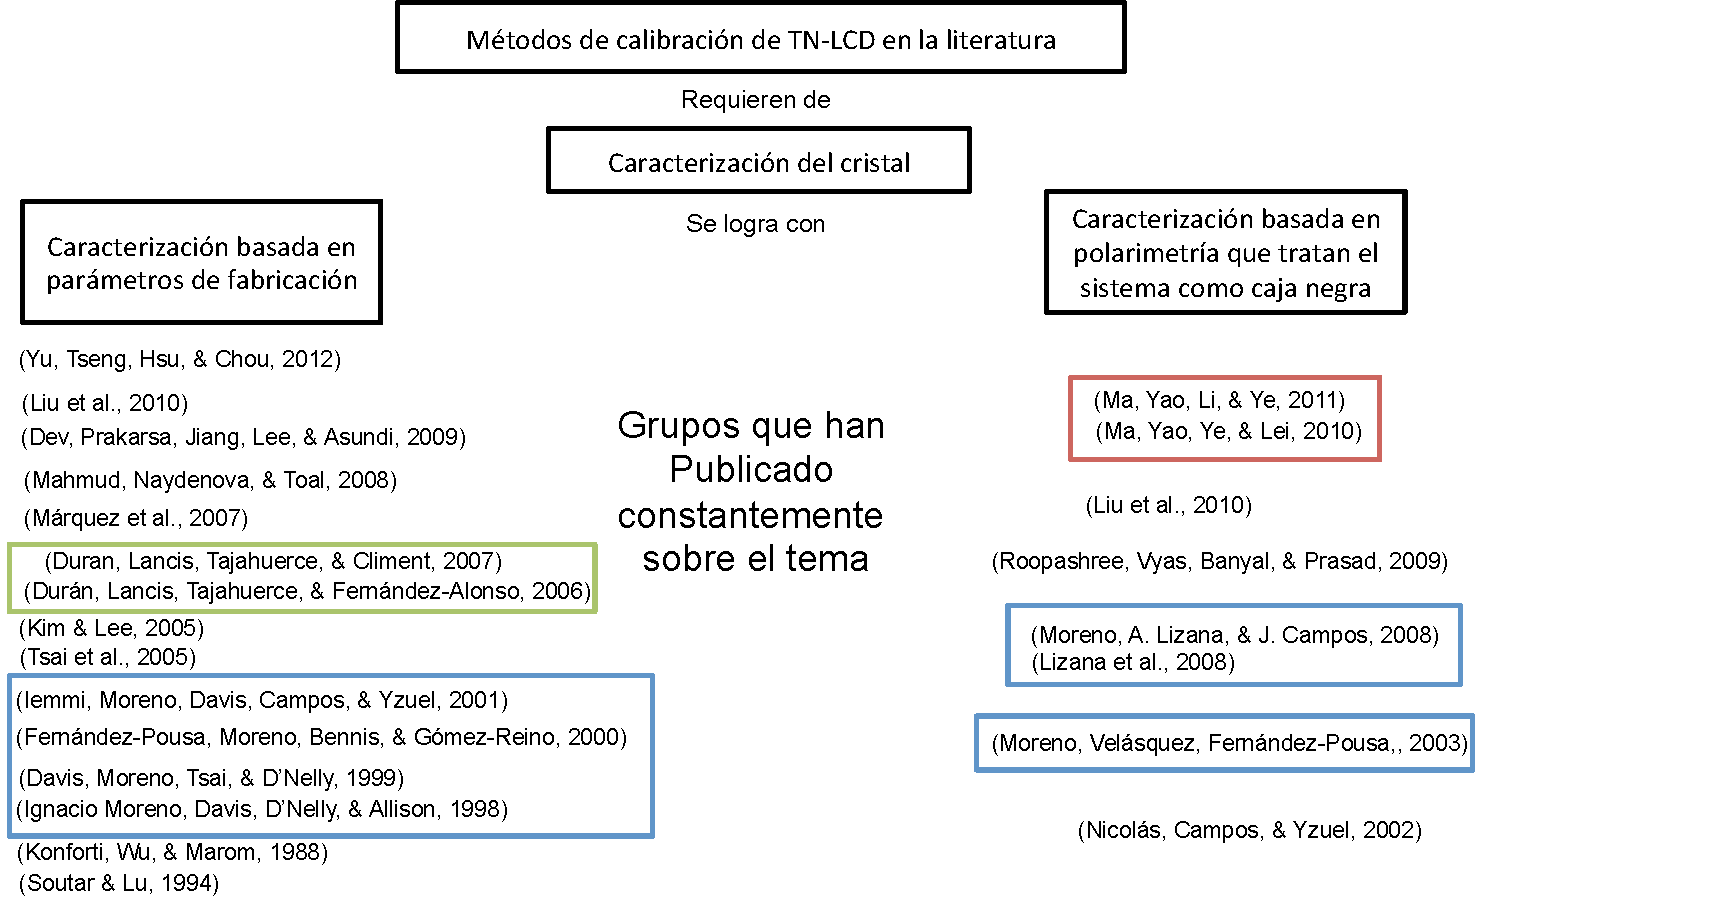
\includegraphics[scale=.6]{articulos_metodos}
\caption[Publicaciones en relación a la caracterización de TN-LCD]{Tabla de publicaciones en relación con caracterización de
  moduladores tipo TN-LCD. Los rectángulos representan los grupos que
  han publicado más en el tema y que resultan de mayor interés para
  este trabajo. }
\label{fig:articulos_metodos}
\end{figure}
El principal resultado del estudio del estado del arte fue encontrar
un patrón en la evolución del tema en la literatura desde los primeros
métodos para pantallas de televisor \citepChGen{Moreno1998} hasta campos
dónde se modula la polarización producidos por moduladores
\citepChGen{Moreno2011}. Este patrón tiene como columna vertebral al 
investigador Ignacio Moreno que, junto con otros investigadores en
universidades de España y California ha dirigido los avances en aplicaciones
científicas de pantallas TN-LCD. 

En lo que sigue de este capítulo presentaremos el resultado de la
caracterizaación de un SLM modelo LC2002 de marca Holoeye con el
método de \citetChGen{Ma2010}.
% una variación del método de caracterización de
% \citetChGen{Moreno2003} implementada por nosotros y que 
%tambien considera el SLM como una caja negra. 
Veremos que la implementación de este método y los resultados
obtenidos involucraron no solo el análisis de datos experimentales sino también el diseño y
construcción de un sistema automatizado para la toma de medidas que se
describe en la sección \ref{sec:instrumento} y el apéndice \ref{AppendixA} 
También se mostrará un método alternativo propuesto por nosotros que
requiere más medidas y permite obtener resultados más veraces. 

Una vez caracterizado el SLM se identificó una combinación de estados
de polarización a la entrada y la salida del SLM que permiten una
modulación de solo fase con la cual se pueden emular elementos
difractivos digitales tales como máscaras espiral de fase, prismas,
lentes de Fresnel e inclusive aberraciones. Los elementos difractivos
producidos de forma digital, y en particular, las máscaras espiral 
 son la clave para producir haces Laguerre-Gauss.  

\chapter{Caracterización de TN-SLM}
\label{cha:Gen_carac}
\label{sec:ChGV_Caracterizacion_de_SLM}
\lhead{Generación de haces Laguerre-Gauss por medio de un SLM: \textit{Caracterización de un TN-SLM}}

Como se mencionó antes, en la caracterización del SLM se pretende
encontrar estados de polarización a la entrada y salida del modulador
que produzcan modulaciones de solo fase, con buena transmitancia y con
un rango amplio de valores de fase. 
Por ende es necesario medir las modulaciones de amplitud y de fase. En
las siguientes secciones se muestra cómo medimos las modulaciones de
amplitud y fase. 

%\subsection{Medida de la modulación de amplitud}
\section{Medida de la modulación de amplitud}
\label{sec:ChGV_med_mod_amp}

En la Fig.~\ref{fig:PSG_PSD} se presenta un esquema del sistema
óptico usado para medir la modulación de amplitud. Si el haz tiene una
polarización lineal y se propaga en la dirección de $z$, la combinación
de un HWP y un primer QWP, conocida como \textbf{generador de estados de
polarización} (\acrshort{PSG}), permite producir estados de polarización
arbitrarios a la entrada del SLM. Luego, el haz llega al SLM y la modulación de amplitud se
debe a que las moléculas de LC en el SLM cambian el estado de
polarización dependiendo del valor de voltaje aplicado. Cuando se añade un \textbf{detector de estados de
polarización} (\acrshort{PSD}) compuesto por un segundo QWP y un polarizador, la amplitud del campo a la salida del polarizador
(P) dependerá de la matriz de Jones del SLM para el nivel de gris
actual y de los vectores de Jones asociados al PSG y PSD. A la salida
del PSD hay un estado con polarización lineal cuya intensidad puede
ser medida usando un fotodetector, o una cámara. 
 \begin{figure}[h!]
\centering
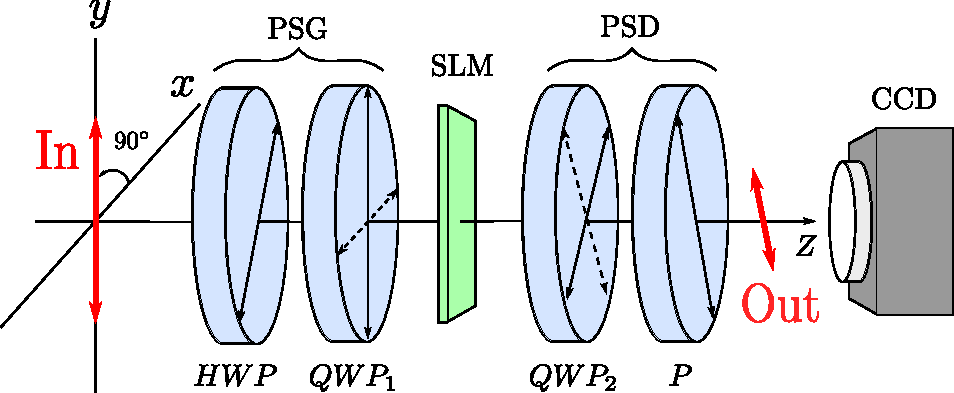
\includegraphics[scale=.8]{PSG_PSD.pdf}
\caption[Esquema de un sistema generador y analizador de estados de
polarización]{Esquema general de un sistema óptico para
  caracterización de modulación de intensidad de un TN-SLM.}
\label{fig:PSG_PSD}
\end{figure}

Desde el punto de vista matemático, el campo a la salida ($Out$) se puede
obtener multiplicando un vector de entrada $In$ por cada uno de
los elementos del sistema 
\begin{equation}
\label{eq:ChGV_Out}
Out = \left( \mathbf{P}\ \mathbf{QWP_2}\ \right) \mathbf{SLM}\ \left( \mathbf{QWP_1}\
\mathbf{HWP}\right)\ In.
\end{equation}
La intensidad medida por la cámara no es más que el módulo cuadrado de
este campo,

\begin{equation}
I = |Out|^2 = Out^{\dagger}Out.
\end{equation}

Luego, en la Fig. \ref{fig:amp_H_V_SLM_2002} se presenta
una curva de modulación de amplitud que se consigue graficando los
valores de intensidad normalizada cuando se varían los niveles de gris discretos
del SLM de 0 a 255. Como se mencionó antes, el nivel de gris es
proporcional al voltaje sobre las celdas de CL y corresponde a 0
cuando el ángulo de inclinación de las moléculas es de 90º con
respecto a la dirección de propagación. La
Fig.~\ref{fig:amp_H_V_SLM_2002} es especialmente interesante porque
muestra el comportamiento del SLM marca Holoeye modelo LC2002 en la
configuración típica de pantallas LCD para proyección, es decir, cuando
el PSG genera un estado de polarización a la entrada vertical y el
PSD detecta un estado horizontal. Como es de esperarse, en esta
configuración el SLM modula amplitud en un rango de 0 a 1 y con una
pendiente relativamente suave y lineal. 
\begin{figure}[h!]
\centering
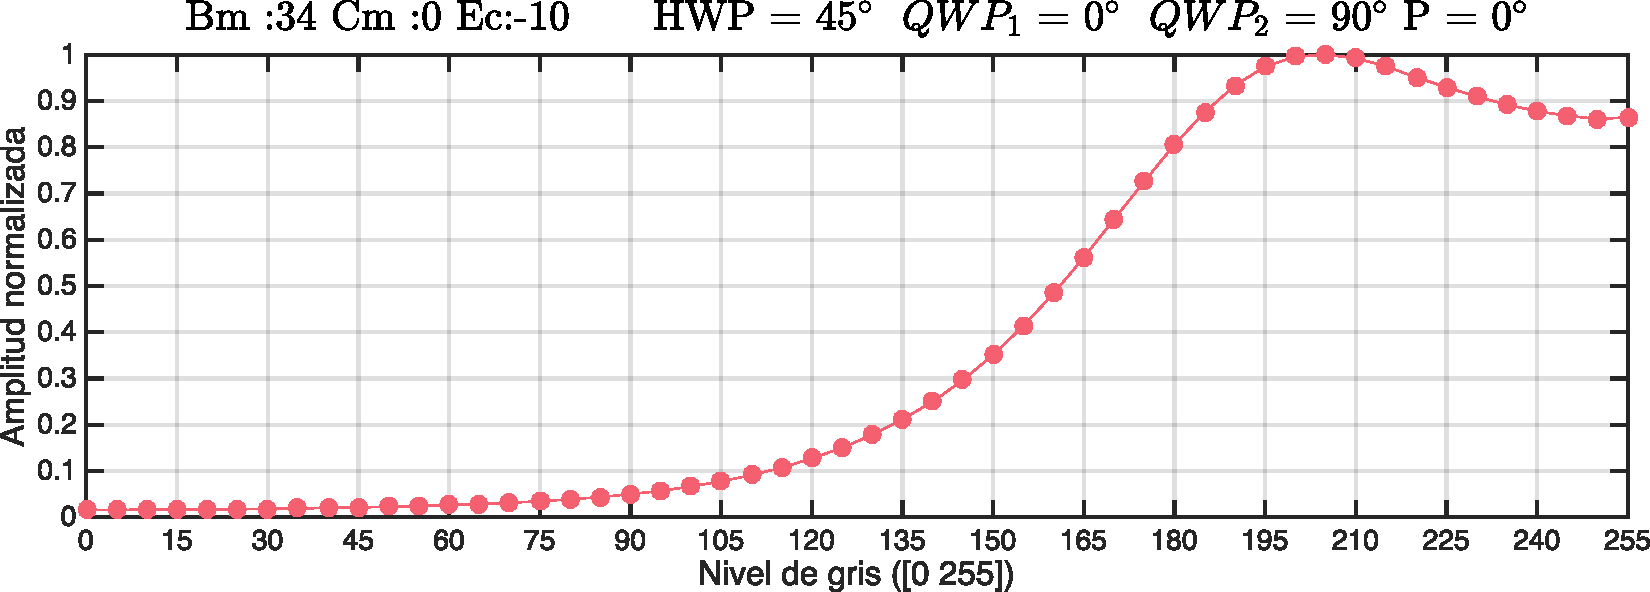
\includegraphics[scale=.55]{amp_H_V_SLM_2002.pdf}
\caption[Curva de modulación de amplitud para un estado no
óptimo]{Medida de la intensidad normalizada del SLM Holoeye LC-2002 en la configuración típica
  de pantallas LCD para proyección. Los primeros tres valores de la parte superior indican la
configuración de brillo (Bm) y contraste (Cm) del SLM, así como la
exposición de la cámara (Ec). Los siguientes 4 indican las posiciones
de los elementos ópticos usados para generar y detectar
estados de polarización.}
\label{fig:amp_H_V_SLM_2002}
\end{figure}
Este tipo de modulaciónes
sirven para proyectar imágenes en niveles de gris y se pueden lograr
con dos polarizadores como PSG y PSD que generen estados lineales ortogonales
entre si.
% Como se explicó en la sección \ref{sec:Propiedades_opticas_de_TNLCD}
%  si el ángulo de torsión de las moléculas en el SLM es de $90^{\circ}$ y
% las moléculas a la entrada están alineadas con el eje horizontal, el
% estado de polarización a la salida será aproximadamente vertical.
No obstante, nuestro objetivo es encontrar una combinación de estados
de polarización que resulten en una baja modulación de amplitud y
buena transmitancia. 

% \subsection{Medida de múltiples estados para alimentar un modelo de
%  caja negra.}
%\label{sec:ChGV_med_mod_amp}
La curva de la Fig. \ref{fig:amp_H_V_SLM_2002} caracteriza la modulación de amplitud del SLM para
una sola combinación de PSG y PSD. Una forma de buscar buenas
combinaciones de PSG y PSD consiste en plantear muchos estados
distintos y medir la modulación hasta encontrar un estado que produzca
los efectos deseados. Hacer esto experimentalmente es un proceso
engorroso y requiere de mucho tiempo porque hay muchas combinaciones
posibles que implican rotar elementos ópticos de forma precisa y con
alta repetibilidad. 
En cambio, vamos a medir experimentalmente sólo 6 combinaciones de PSG
y PSD propuestas por \citetChGen{Ma2010} y con
ellas alimentaremos un modelo analítico y otro modelo numérico con los
cuales se obtienen los parámetros de la matriz de 
Jones para cada nivel de gris por medio de operaciones aritméticas
simples en el caso del primero, y funciones de minimización en el segundo.
% serán encontrada por un método de ajuste
% de parámetros.
% de caja negra 
% basado en un algoritmo de minimización basado en la búsqueda del
% gradiente. 
Una vez conocido el modelo del SLM se puede buscar el
estado que mejor satisface las condiciones de operación haciendo simulaciones con
las cuales sí es práctico hacer una búsqueda entre múltiples estados.

A continuación se introducirá una notación alternativa para la
representación de estados de polarización que es de uso generalizada
en las referencias consultadas \citepChGen{Moreno2003,Ma2010} (entre
otras) y que facilita la
representación de las combinaciones de PSG y PSD para medidas de
intensidad.  

%\subsubsection{La notación de Dirac}
\subsection{La notación de Dirac}
De forma similar a cómo sucede en la mecánica cuántica, los estados de
polarización arbitrarios generados por un PSG se pueden representar en
la notación de BraKets de Dirac como Ket's:
\begin{equation}
|J> = \begin{pmatrix} J_x \\ J_y\end{pmatrix} = \left( \mathbf{QWP_1}\
\mathbf{HWP}\right)\ In.
\end{equation}
Y siguiendo esta interpretación, el PSD correspondiente a un PSG dado
es el Bra, es decir, el vector que es complejo conjugado de un Ket
\begin{equation}
<J|= |J>^{\dagger} = \begin{pmatrix} J_x^* &  J_y^*\end{pmatrix}. 
\end{equation}
Por otra parte, la matriz de Jones del SLM cumple el papel que tendría un
operador en la mecánica cuántica. Si los Bra y Ket representan vectores normalizados, la
intensidad del campo a la salida puede ser obtenida como el módulo
cuadrado del valor
esperado del operador del SLM  (Eq. \ref{eq:general_jones_matrix})
cuando la base del PSG es proyectada sobre la del PSD \citepChGen{Moreno2003,Ma2010}.
\begin{align}
\label{eq:valor_esperado}
I = |<J|\mathbf{SLM} |J>|^2 &= 
\begin{pmatrix}
J_x & J_y
\end{pmatrix}
\begin{pmatrix}
A & B\\
 -B^* & A^* 
\end{pmatrix}
\begin{pmatrix}
J_x \\ J_y
\end{pmatrix}
,\nonumber\\
&= 
\begin{pmatrix}
J_x & J_y
\end{pmatrix}
\begin{pmatrix}
X+iY & Z+iW\\
 -Z+iW & X-iY 
\end{pmatrix}
\begin{pmatrix}
J_x \\ J_y
\end{pmatrix}
.
\end{align}
%donde $A$ y $B$ son números complejos.

La intensidad es una variable que se puede medir con una cámara o fotodiodo, y los vectores
correspondientes a los estados producidos por el PSG y el PSD son
conocidos. Como los vectores de Jones que utilizamos están
normalizados, lo más adecuado es normalizar también las medidas de
intensidad. Una forma de normalizar las medidas consiste en medir no
solo el BraKet deseado sino también un Braket en el cual el Bra o PSD es un
vector ortogonal al PSD original.  La intensidad medida con el PSD
ortogonal es entonces un complemento de la original y su suma debe ser
un valor constante. Si se divide cualquiera de las dos intensidades experimentales
sobre la suma de las dos, obtenemos un valor que ha sido
normalizado y que es equivalente a aquellos obtenidos usando del producto
analítico de la Eq. \ref{eq:valor_esperado}, 

\begin{align*}
\hat{I} &= \frac{I}{I+I^{\perp}},&\hat{I}^{\perp} &= \frac{I^{\perp}}{I+I^{\perp}}.
\end{align*}

%\subsubsection{El método de Ma et al.}
\section{El método de Ma et al.~ para la caracterización del SLM}
\label{sec:metodo_ma}
Según \citetChGen{Ma2010}, hay tres combinaciones de PSD y PSG a partir
de las cuales se pueden encontrar los valores X,Y,Z, y W de la matriz
de Jones de un SLM. Si para
normalizar cada una de ellas requerimos medir otra en la cual el Bra
es el vector ortogonal del Bra original, se requiere de las siguientes
6 medidas, 
\begin{align*}
I_1 &= |<\mathbf{H}|SLM|\mathbf{H}>|^2,& I_2 &= |<\mathbf{CD}|SLM|\mathbf{CD}>|^2,&I_3
  &= |<\mathbf{45^{\circ}}|SLM|\mathbf{45^{\circ}}>|^2,\\
I_1^{\perp} &= |<\mathbf{V}|SLM|\mathbf{H}>|^2,&I_2^{\perp} &= |<\mathbf{CI}|SLM|\mathbf{CD}>|^2,&I_{3}^{\perp} &= |<\mathbf{-45^{\circ}}|SLM|\mathbf{45^{\circ}}>|^2.
\end{align*}
Dónde el símbolo $^{\perp}$ denota ortogonalidad, y básicamente se
está midiendo qué tan transparente es el SLM ante 
los estados vertical, circular derecho, y lineal a $45^{\circ}$. 
Estas tres medidas son interesantes porque se puede encontrar una
relación entre la intensidad medida 
y los valores desconocidos de la matriz de Jones. 
A continuación se muestra el procedimiento matemático expuesto por Ma
et al.~que relaciona cada una de las intensidades con los valores de
la matriz de Jones. 
Analizar la transmitancia ante el estado lineal horizontal entrega un valor
de intensidad que es función de $X$ y $Y$,
\begin{align*}
I_1 = |<\mathbf{H}|SLM|\mathbf{H}>|^2 &= X^2+Y^2,\\
&=  \left|\begin{pmatrix} 1&0\end{pmatrix} 
       \begin{pmatrix}
         X+iY & Z+iW \\-Z+iW & X-iY
       \end{pmatrix} \begin{pmatrix}1\\0\end{pmatrix}\right|^2, \\
&=  \left|\begin{pmatrix} 1&0\end{pmatrix} 
       \begin{pmatrix} X+iY \\-Z+iW \end{pmatrix} \right|^2, \\
&=  \left|X+iY\right|^2 =  X^2+Y^2.\\
\end{align*}
Y analizar la transmitancia ante un estado circular derecho entrega un
valor de intensidad función de $X$ y $Z$.
\begin{align*}
I_2 = |<\mathbf{CD}|SLM|\mathbf{CD}>|^2 &= X^2+Z^2,\\
&=  \left|\frac{1}{\sqrt{2}}\begin{pmatrix} 1&-i\end{pmatrix} 
       \begin{pmatrix}
         X+iY & Z+iW \\-Z+iW & X-iY
       \end{pmatrix} \frac{1}{\sqrt{2}}\begin{pmatrix}1\\i\end{pmatrix}\right|^2 ,\\
&=  \left|\frac{1}{2}\begin{pmatrix} 1&-i\end{pmatrix} 
       \begin{pmatrix} X+iY +iZ-W\\-Z+iW +iX+Y\end{pmatrix} \right|^2 ,\\
&=  \left|\frac{1}{2}\left(X+iY+iZ-iW+iZ+W+X-iY\right)\right|^2 =  X^2+Z^2.\\
\end{align*}
Como en los casos anteriores, se muestra que la intensidad medida
cuando se genera y detecta un estado inclinado a $45^{\circ}$ depende
ahora de $X$ y $W$.
\begin{align*}
I_3 = |<\mathbf{45^{\circ}}|SLM|\mathbf{45^{\circ}}>|^2 &= X^2+W^2,\\
&=  \left|\frac{1}{\sqrt{2}}\begin{pmatrix} 1&1\end{pmatrix} 
       \begin{pmatrix}
         X+iY & Z+iW \\-Z+iW & X-iY
       \end{pmatrix} \frac{1}{\sqrt{2}}\begin{pmatrix}1\\1\end{pmatrix}\right|^2 ,\\
&=  \left|\frac{1}{2}\begin{pmatrix} 1&1\end{pmatrix} 
       \begin{pmatrix} X+iY +Z+iW\\-Z+iW +X-iY\end{pmatrix} \right|^2, \\
&=  \left|\frac{1}{2}\left(X+iY+Z+iW-Z+iW+X-iY\right)\right|^2 =  X^2+W^2.\\
\end{align*}
Adicionalmente, de la Eq. \ref{eq:unimodular} podemos deducir la siguiente condición de
normalización que está relacionada con el hecho de ser una matriz
unitaria y por ende unimodular,
\begin{equation*}
X^2+Y^2+Z^2+W^2 =1.
\end{equation*}
Con esta última relación tenemos 4 ecuaciones para 4 incógnitas, y
tras realizar operaciones simples de sustitución podemos despejar
$X^2$, $Y^2$, $Z^2$ y $W^2$ en función de $I_1$, $I_2$, y $I_3$,
\begin{align*}
X^2 &= \frac{1}{2}\left( I_1+I_2+I_3-1\right), & Y^2 &=
                                                       \frac{1}{2}\left(
                                                       I_1-I_2-I_3+1\right),\\
Z^2 &= \frac{1}{2}\left( I_2-I_1-I_3+1\right), & W^2 &=
                                                       \frac{1}{2}\left(
                                                       I_3-I_1-I_2+1\right).\\
\end{align*}

Nosotros medimos estas tres intensidades para 52 de los 255 niveles de
gris del SLM y obtuvimos curvas muy similares a las de \citetChGen{Ma2014}. La
comparación entre las medidas de intensidad normalizadas y las de Ma se observa en la
Fig. \ref{fig:Ma_and_our_Is}.
\begin{figure}[h!]
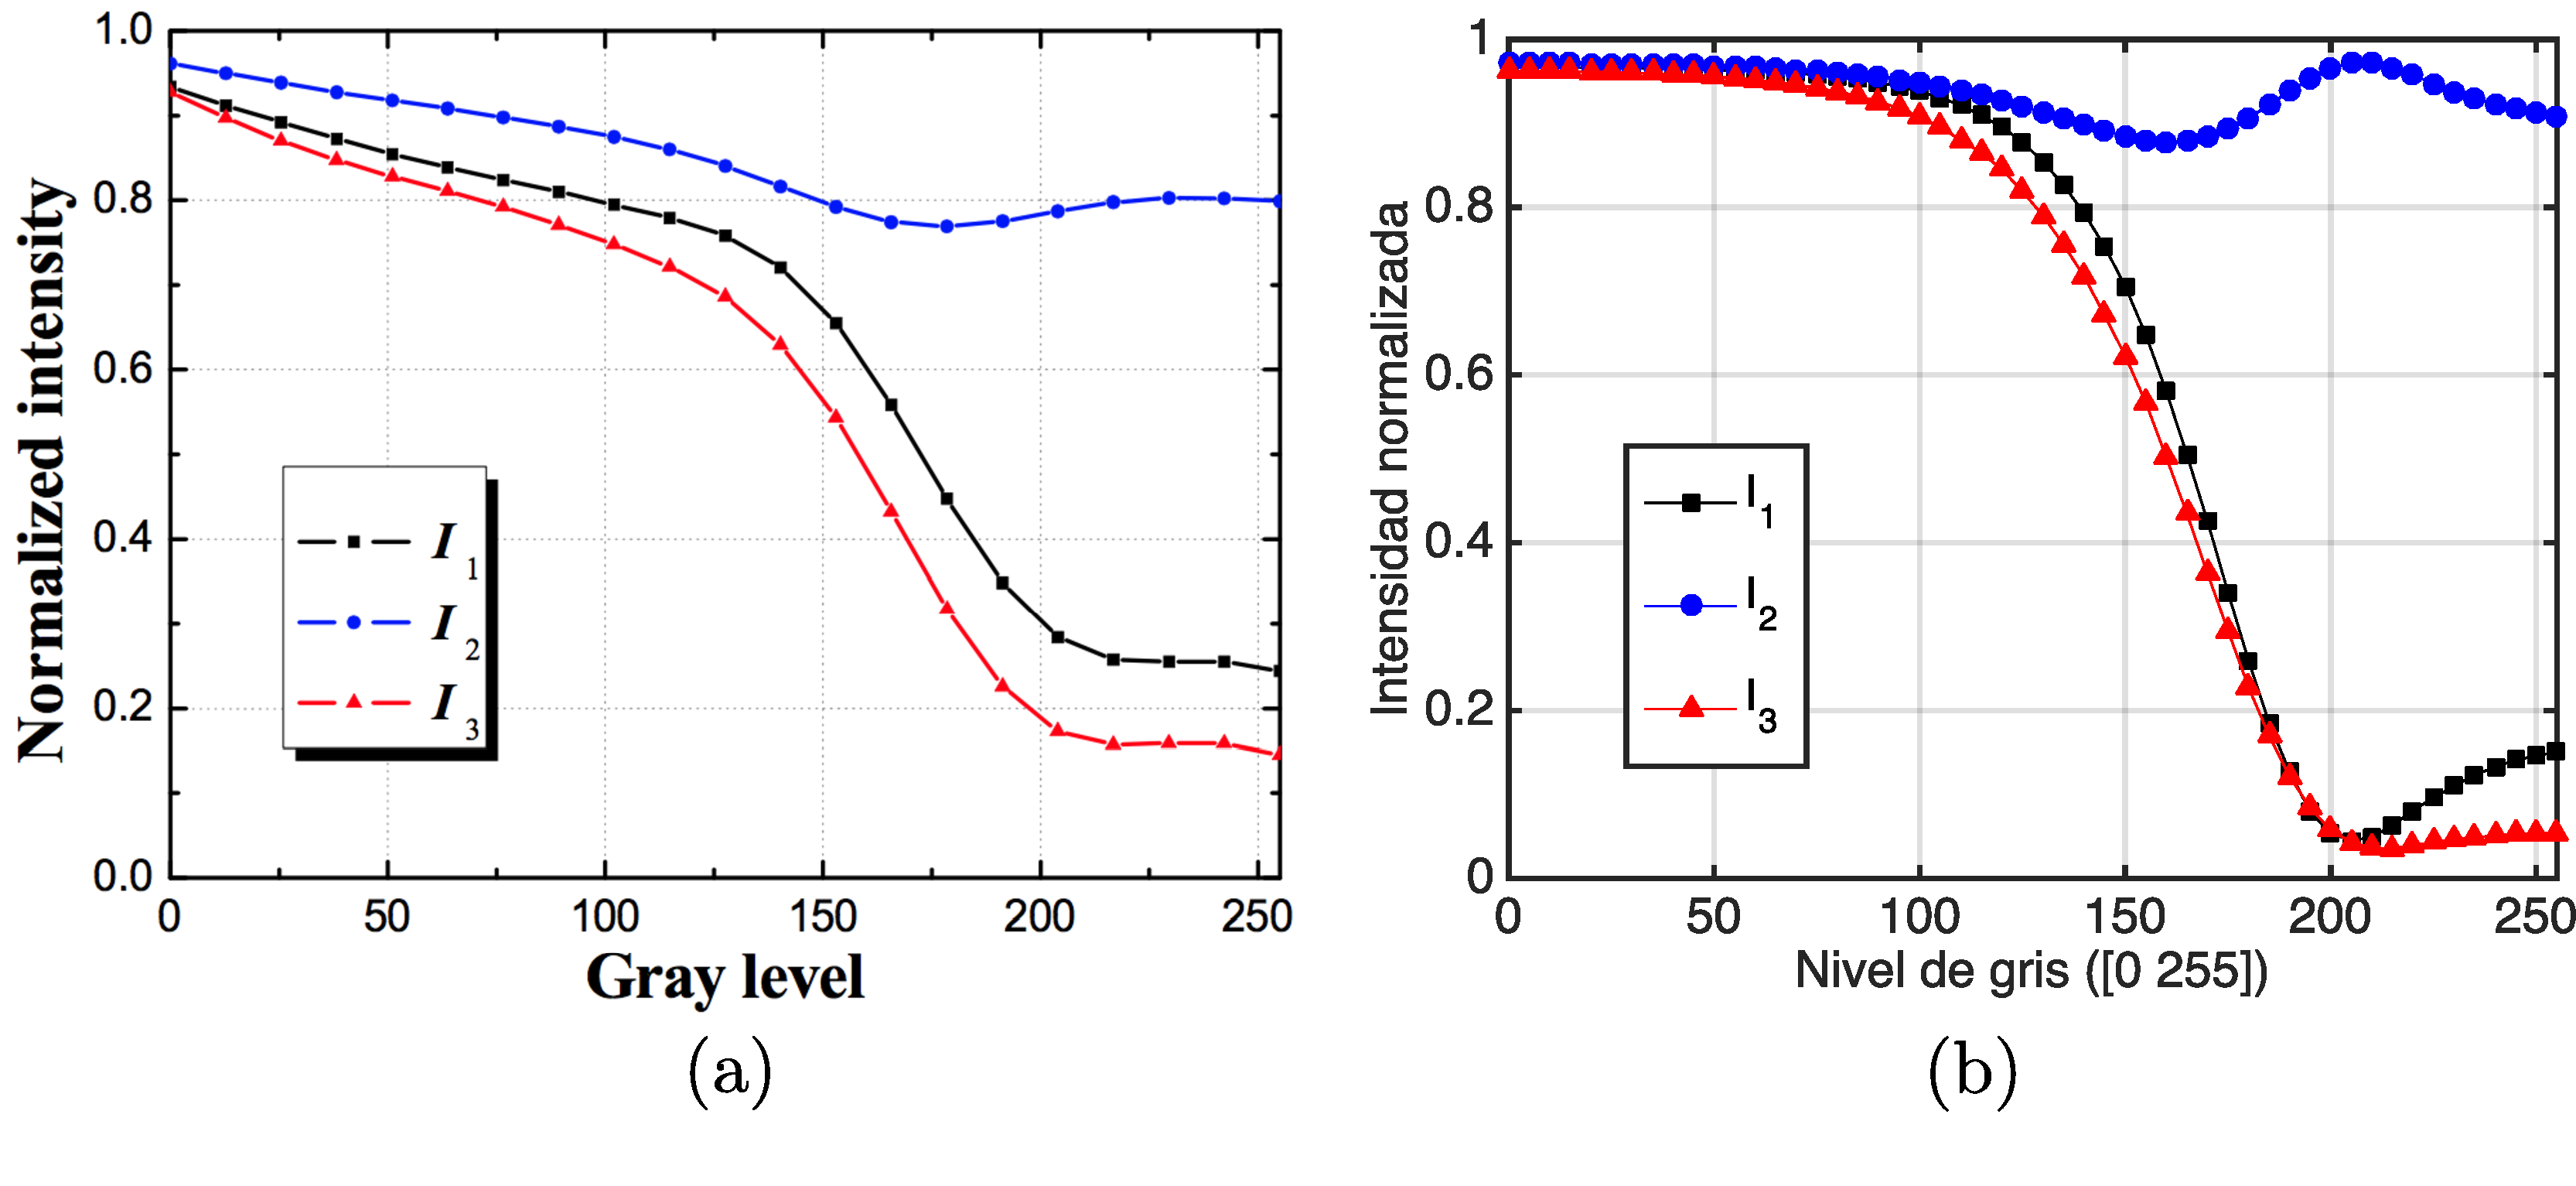
\includegraphics[scale = .27]{Ma_and_our_Is.pdf}
\caption[Comparación entre las tres intensidades para calibración
medidas por Ma et al.~ para un SLM similar y por
nosotros.]{Comparación entre las tres intensidades para calibración 
medidas por \citetChGen{Ma2014}~ (a) y por nosotros (b).}
\label{fig:Ma_and_our_Is}
\end{figure}
Asimismo, calculamos los valores de los cuadrados de los parámetros de
Jones siguiendo las ecuaciones mencionadas y obtuvimos los resultados
presentados en la Fig. \ref{fig:Our_Ma_X2Y2Z2W2}. 
\begin{figure}[h!]
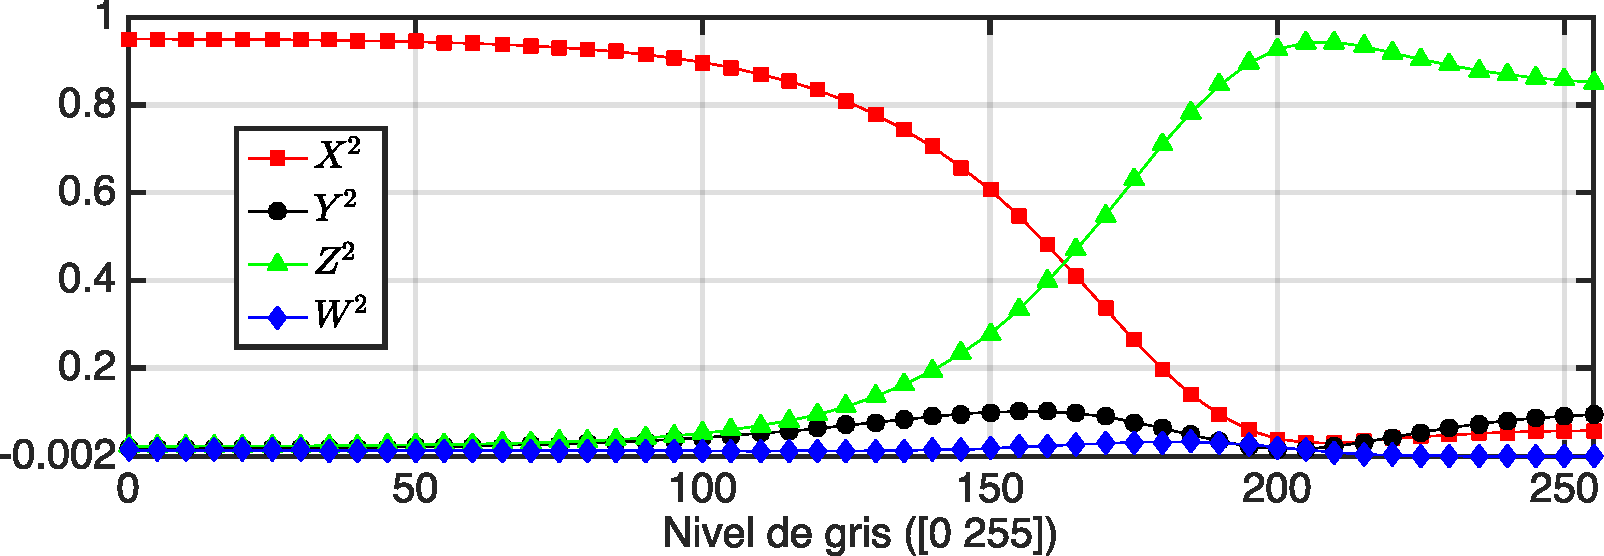
\includegraphics[scale = .55]{Our_Ma_X2Y2Z2W2_long.pdf}
\caption[Valores de $X^2$, $Y^2$ $Z^2$ y $W^2$ encontrados por
nosotros utilizando el método de Ma et al.]{Valores de $X^2$, $Y^2$ $Z^2$ y $W^2$ encontrados por
nosotros utilizando el método de Ma et al.}   
\label{fig:Our_Ma_X2Y2Z2W2}
\end{figure}
Una primera dificultad que identificamos aplicando el método de Ma fue
la ausencia de un mecanismo para definir el signo de la raíz
cuadrada de $X^2$, $Y^2$, $Z^2$ y $W^2$. Por otra parte, observamos
que aproximadamente a partir del nivel 200 la curva de $Y^2$ cambia de
direcci'on sugiriendo un cambio de signo en $Y$ y aparecen valores negativos
en la curva del parámetro $W^2$. Lo segundo produce raíces complejas no
permitidas por la teoría, y puede ser debido a variaciones leves
en la intensidad registrada por la cámara. La presencia de
valores negativos no es discutida en los artículos consultados y no
hemos identificado una restricción teórica que impida observar este
fenomeno al hacer las restas de las intensidades. Con el fin de
obtener un resultado similar al de \citetChGen{Ma2014} asumimos
  que $Z$ y $W$ son negativos y calculamos el parámetro $W$ como
  $W=\sqrt{|W^2|}$ para evitar valores complejos. Nuestros
  resultados se comparan con los de Ma et al en la Fig. \ref{fig:Ma_and_our_XYZW}.
\begin{figure}[h!]
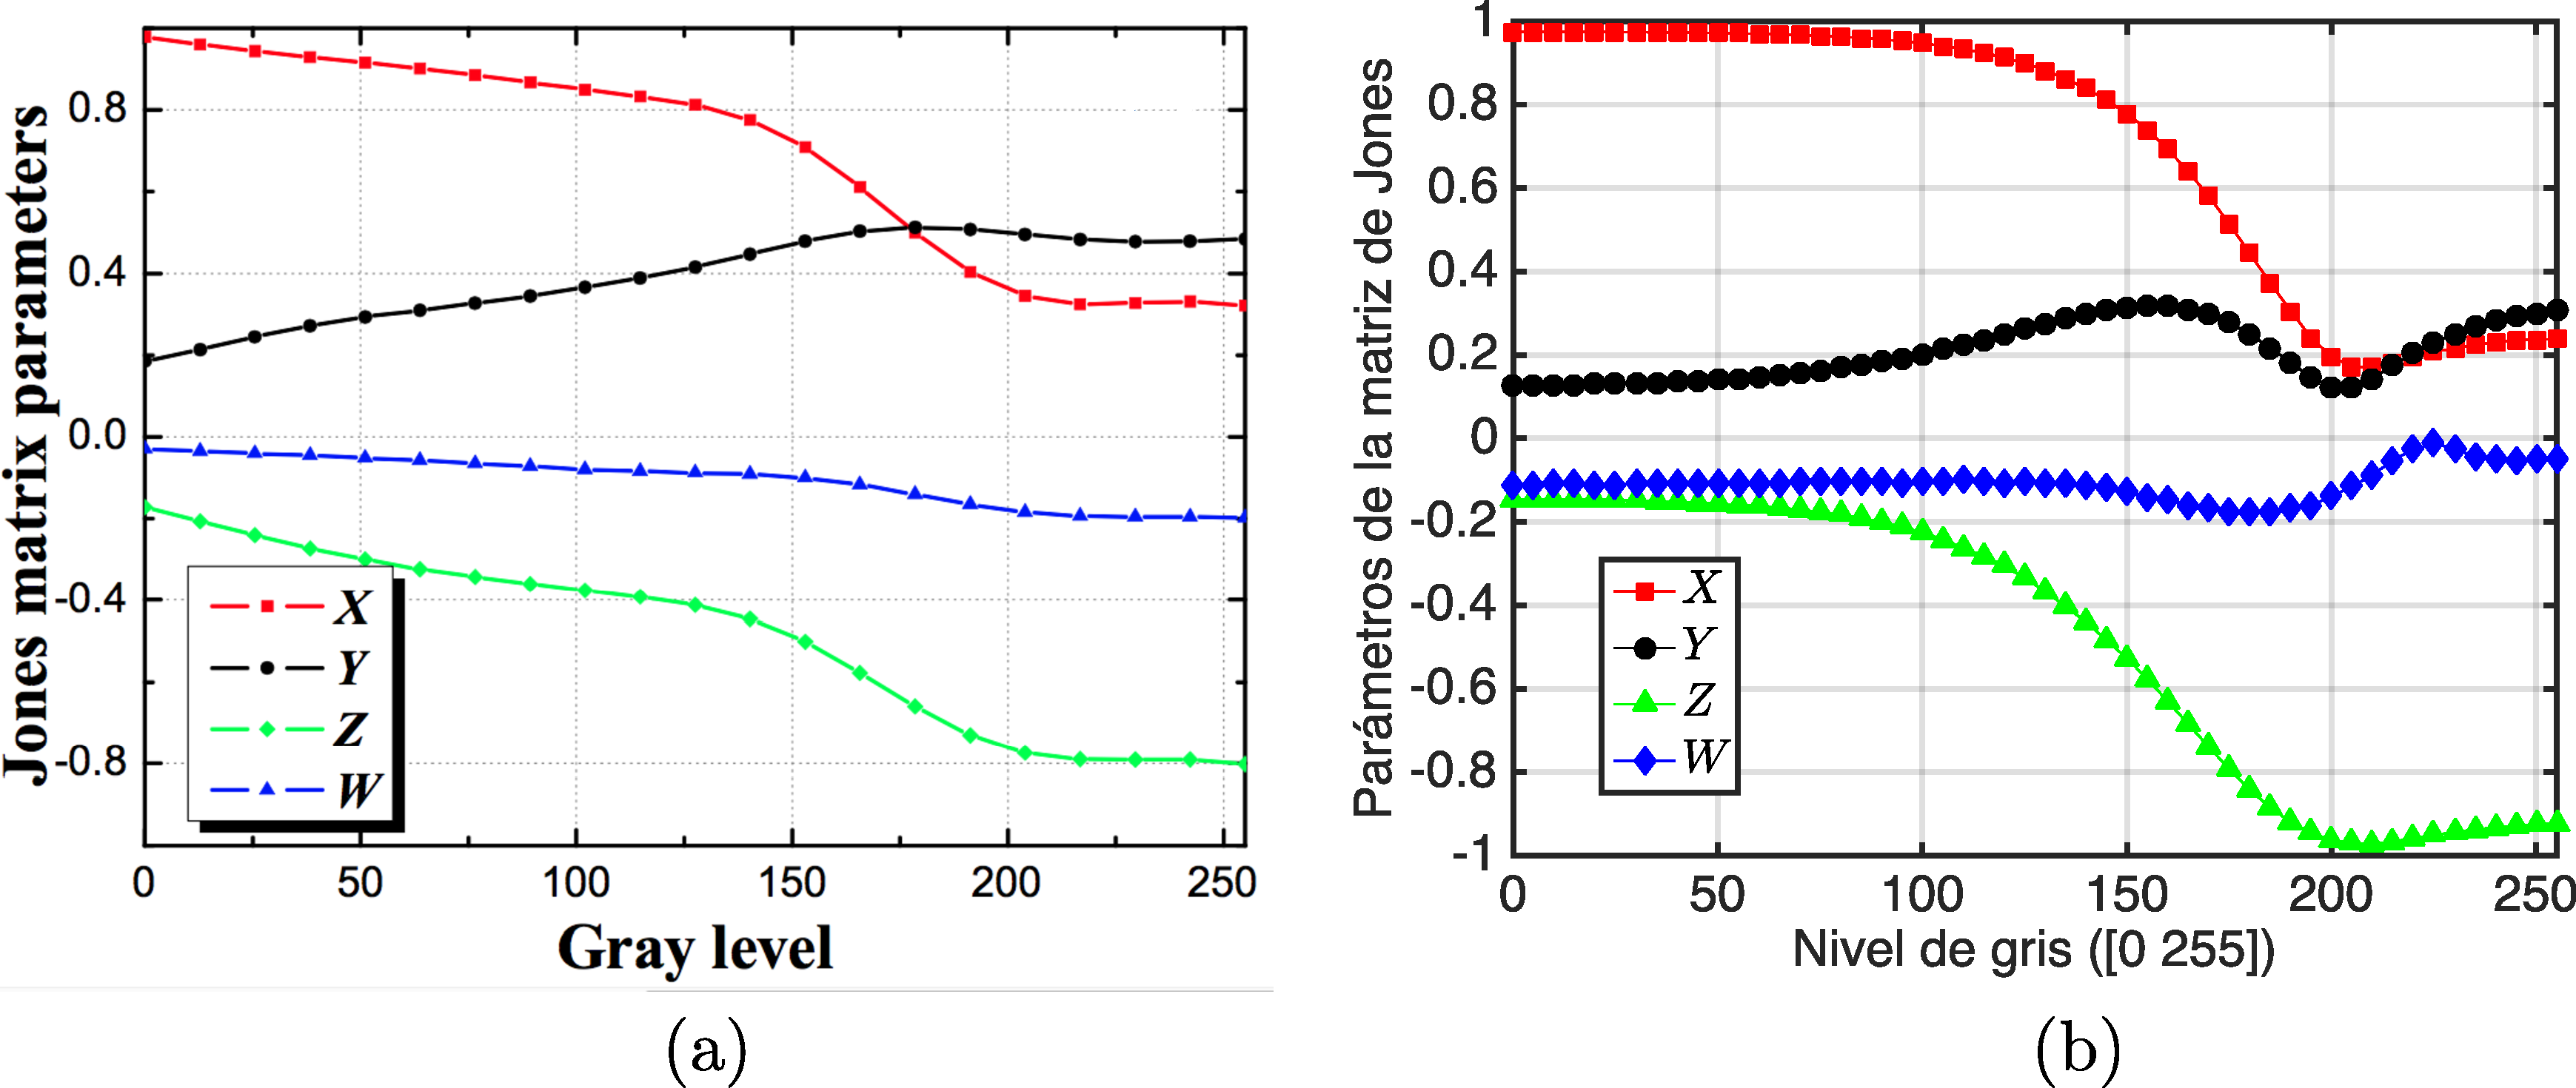
\includegraphics[scale = .26]{Ma_and_our_XYZW.pdf}
\caption[Comparación entre los valores de $X$, $Y$ $Z$ y $W$ encontrados por
Ma et al.~ para un SLM similar y por nosotros.]{Comparación entre los
  valores de X, Y Z y W encontrados por \citetChGen{Ma2014}~ 
  (a) y por nosotros (b). Dado que no queda explícito cómo encontrar
  el signo de los parámetros en ninguna de sus publicaciones, asumimos
  que $Z$ y $W$ son negativos como ellos lo presentan.}   
\label{fig:Ma_and_our_XYZW}
\end{figure}
En primera medida, en la Fig. \ref{fig:Ma_and_our_XYZW} se observa que
las curvas de los parámetros $X$, y 
$Y$ siguen la misma tendencia descendente que la encontrada por
\citetChGen{Moreno2003}, dónde la matriz comienza siendo muy similar a
una matriz identidad con $X$ cercano a uno y el resto de parámetros
tendientes a cero. Por otra parte, y también de acuerdo con otros
autores \citepChGen{Saleh1990,Marquez2000} se observan valores de $W$
cercanos a cero y valores de $Y$ 
que aumentan proporcionalmente al nivel de gris. El hecho de que $W$
sea muy cercano a cero es consistente con el modelo basado en los
parámetros físicos del modulador de
\citetChGen{Marquez2000} y con la
Eq. \ref{eq:TN-LCD_Jones_Matrix} derivada en la sección
\ref{sec:Propiedades_opticas_de_TNLCD} de este documento. 

\subsection{Comprobación experimental con 100 medidas}
\label{sec:exp_validation}
Hemos comparado las intensidades predichas por las matrices obtenidas
y encontramos que el modelo emula con muy buena exactitud tanto las 3 medidas
de entrada como las 3 medidas ortogonales. Para cada uno de los 6
estados el error absoluto promedio es menor a $2\times10^{-4}$.  Se
calcula el error absoluto promedio para cada estado como,
\begin{equation*}
error_i = \sum_{n=1}^{52}\frac{|I_n^e-I_n^s|}{52}.
\end{equation*}   
No obstante, observamos que la predicción del modelo no tiene una
exactitud igual de buena para estados distintos a los estados usados
para la caracterización. 
Con el fin de comprobar que las matrices obtenidas eran un modelo adecuado
del SLM se hicieron 100 medidas nuevas de modulación de amplitud y se
compararon con las simuladas. En esas medidas se hicieron todas las combinaciones
posibles entre 10 vectores Ket y Bra usando la 
numeración que se esquematiza en la Fig. \ref{fig:braket_100_notation}.
\begin{figure}[h!]
\centering
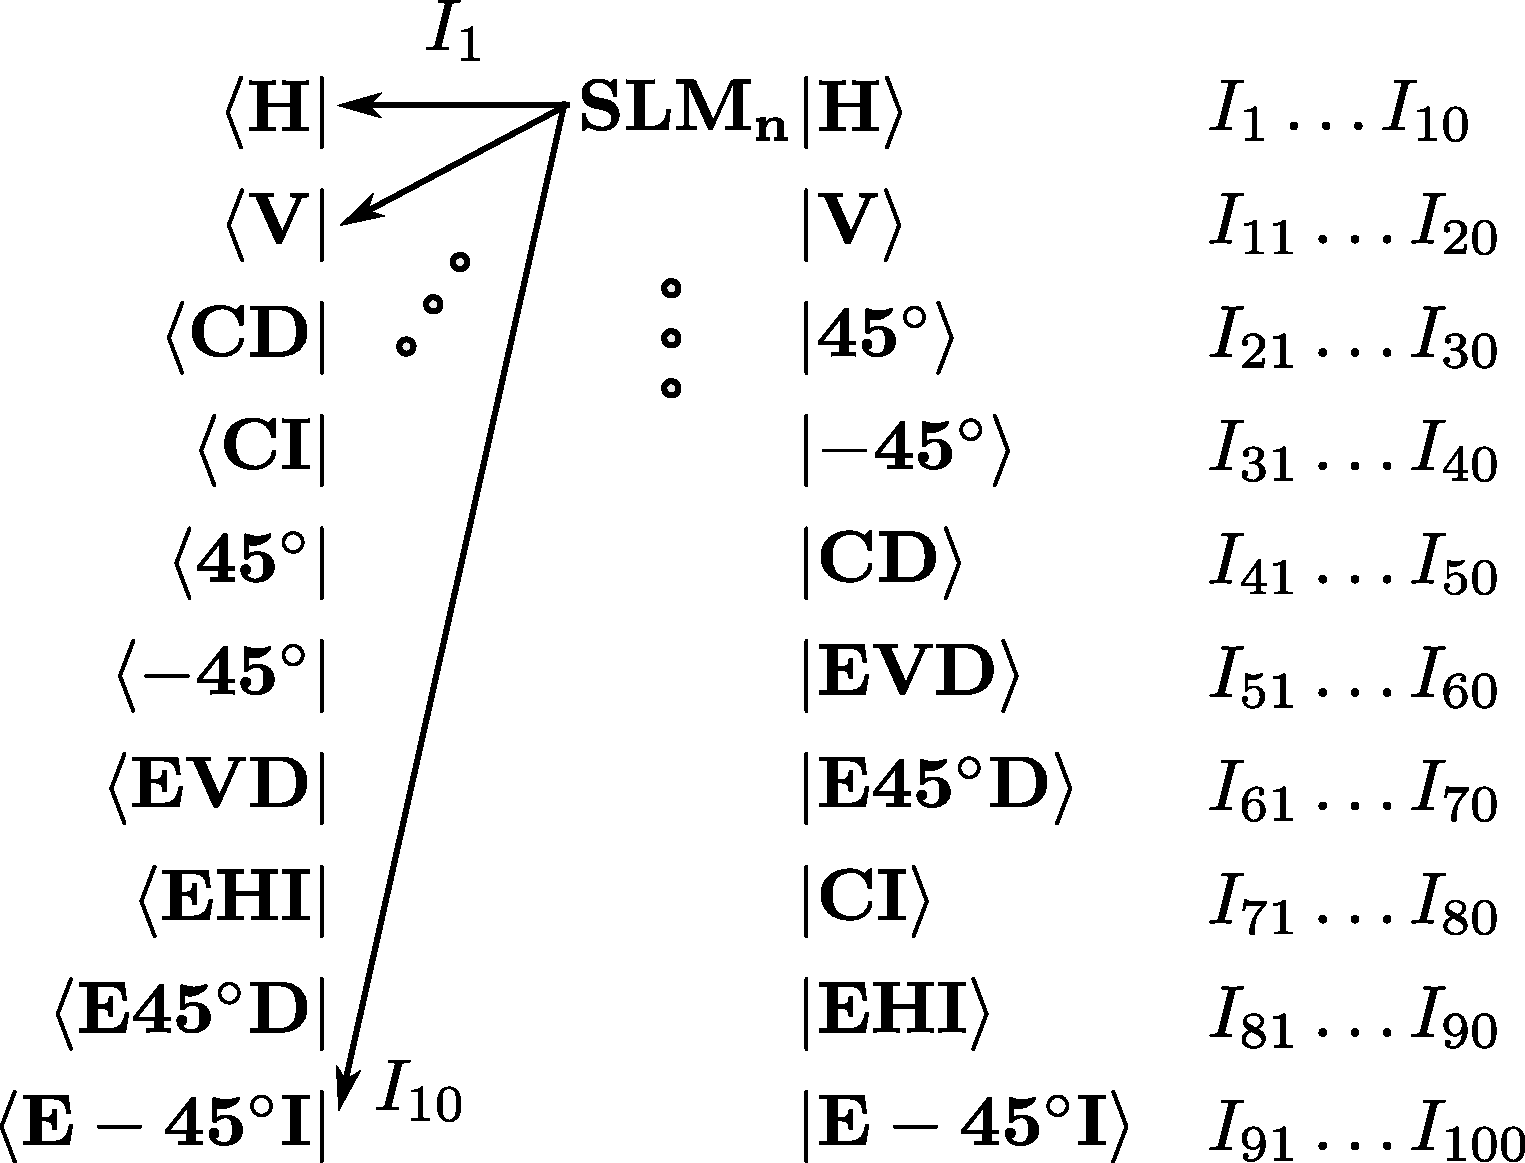
\includegraphics[scale=.4]{brakets.pdf}
\caption[Numeración de medidas experimentales de modulación para
corroboración del modelo de SLM]{Numeración de medidas experimentales de modulación para
corroboración del modelo del SLM. Por cada Ket hay 10 Bra y la
numeración se hace entre parejas en orden descendente con los pares
representados en la figura. }
\label{fig:braket_100_notation}
\end{figure}
Entre los estados se incluyeron dos parejas de estados
elípticos ortonormales no usados
como entrada del algoritmo de minimización. Los estados elípticos
corresponden a polarizaciones elípticas horizontal, vertical, a
$45^{\circ}$ y a $-45^{\circ}$ con ángulo de elipticidad $\theta
=22.5^{\circ}$ como se muestra en la Fig. \ref{fig:elliptic_states}.
\\
Para saber cómo ubicar los
elementos ópticos que generan y detectan estados de polarización
elípticos arbitrarios usamos un software desarrollado y registrado por nosotros en el Grupo de
Óptica Aplicada y presentado como una ponencia de póster en el evento
\href{http://www.eafit.edu.co/focuslatinoamerica2014/Paginas/Inicio.aspx}{\textbf{FOCUS
    Latinoamérica}} en Noviembre del 2014. El póster junto con la
interfaz gráfica y las librerías pueden ser descargadas sin costo en
el siguiente vínculo web:\\
\hspace*{\fill}
\href{https://github.com/bebopsan/Ellipsometry\_for\_dummies.git}{\textbf{https://github.com/bebopsan/Ellipsometry\_for\_dummies.git}}\hspace*{\fill}.\\

Aún cuando la imprecisión del método se hace evidente de forma
cualitativa, se midió un error promedio global para los
100 estados como medida cuantitativa, $$error_g =
\sum_{i=1}^{100}\frac{error_i}{100},$$ y se obtuvo un valor de $error_g
= 0.085628$. Es decir que con intensidades normalizadas la diferencia
entre la medida y la simulación es de alrededor de $8\%$.
Cuatro de los 100 resultados que incluyen estados elípticos se muestran en la
Fig. \ref{fig:Ma_caracterization_results} y el resto de medidas se han
puesto al alcance del lector como un notebook de iPython en un
repositorio alojado también en GitHub en el enlace: \href{http://goo.gl/69kSu2}{\textbf{http://goo.gl/69kSu2}}. 
Ese vínculo dirige a una copia del archivo que
usamos para cargar y calcular los parámetros de las matrices de Jones
del SLM usando el método de Ma et al.~ Allí se incluye tanto el código
de nuestra implementación como las figuras de los resultados. 
\begin{figure}[h!]
\centering
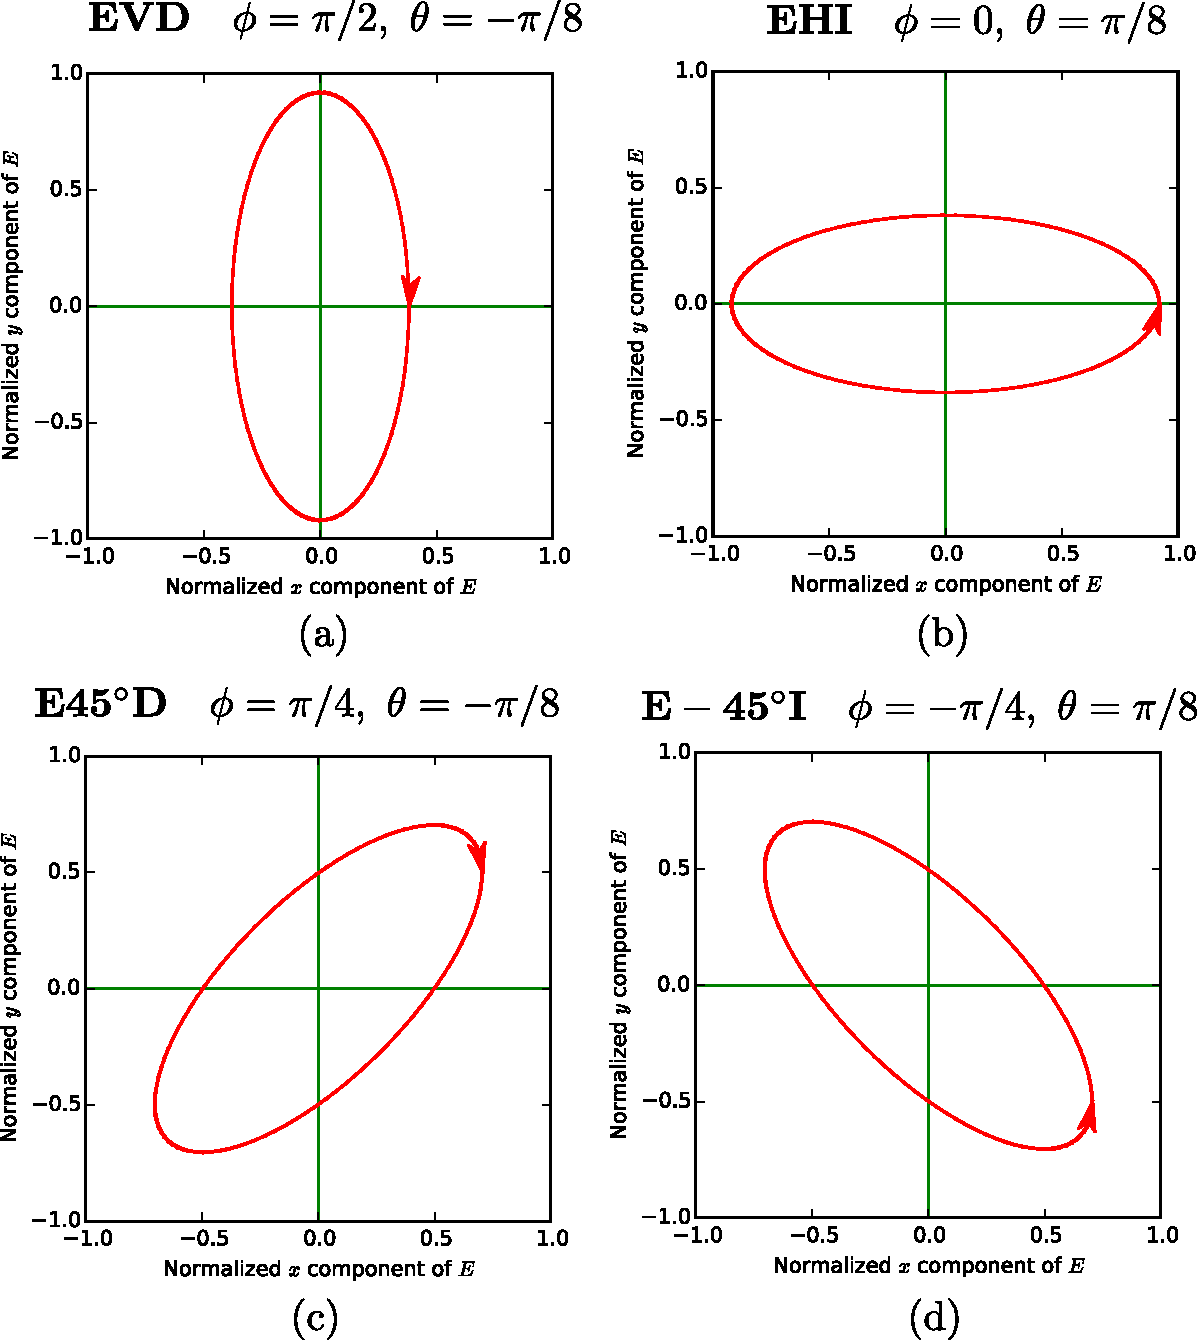
\includegraphics[scale = .6]{EVD_EHI_E45D_Em45I.pdf}
\caption[Estados de polarización elípticos]{Dos pares de estados de polarización
  elípticos ortonormales con ángulo de elipticidad $\theta = 22.5^{\circ}$. (a) Polarización Elíptica Vertical Derecha,
  (b) Elíptica Horizontal Izquierda, (c) Elíptica a $45^{\circ}$
  Derecha, y (d) Elíptica a $-45^{\circ}$ Izquierda.}
\label{fig:elliptic_states}
\end{figure}
%\newpage
\begin{figure}[h!]
\centering
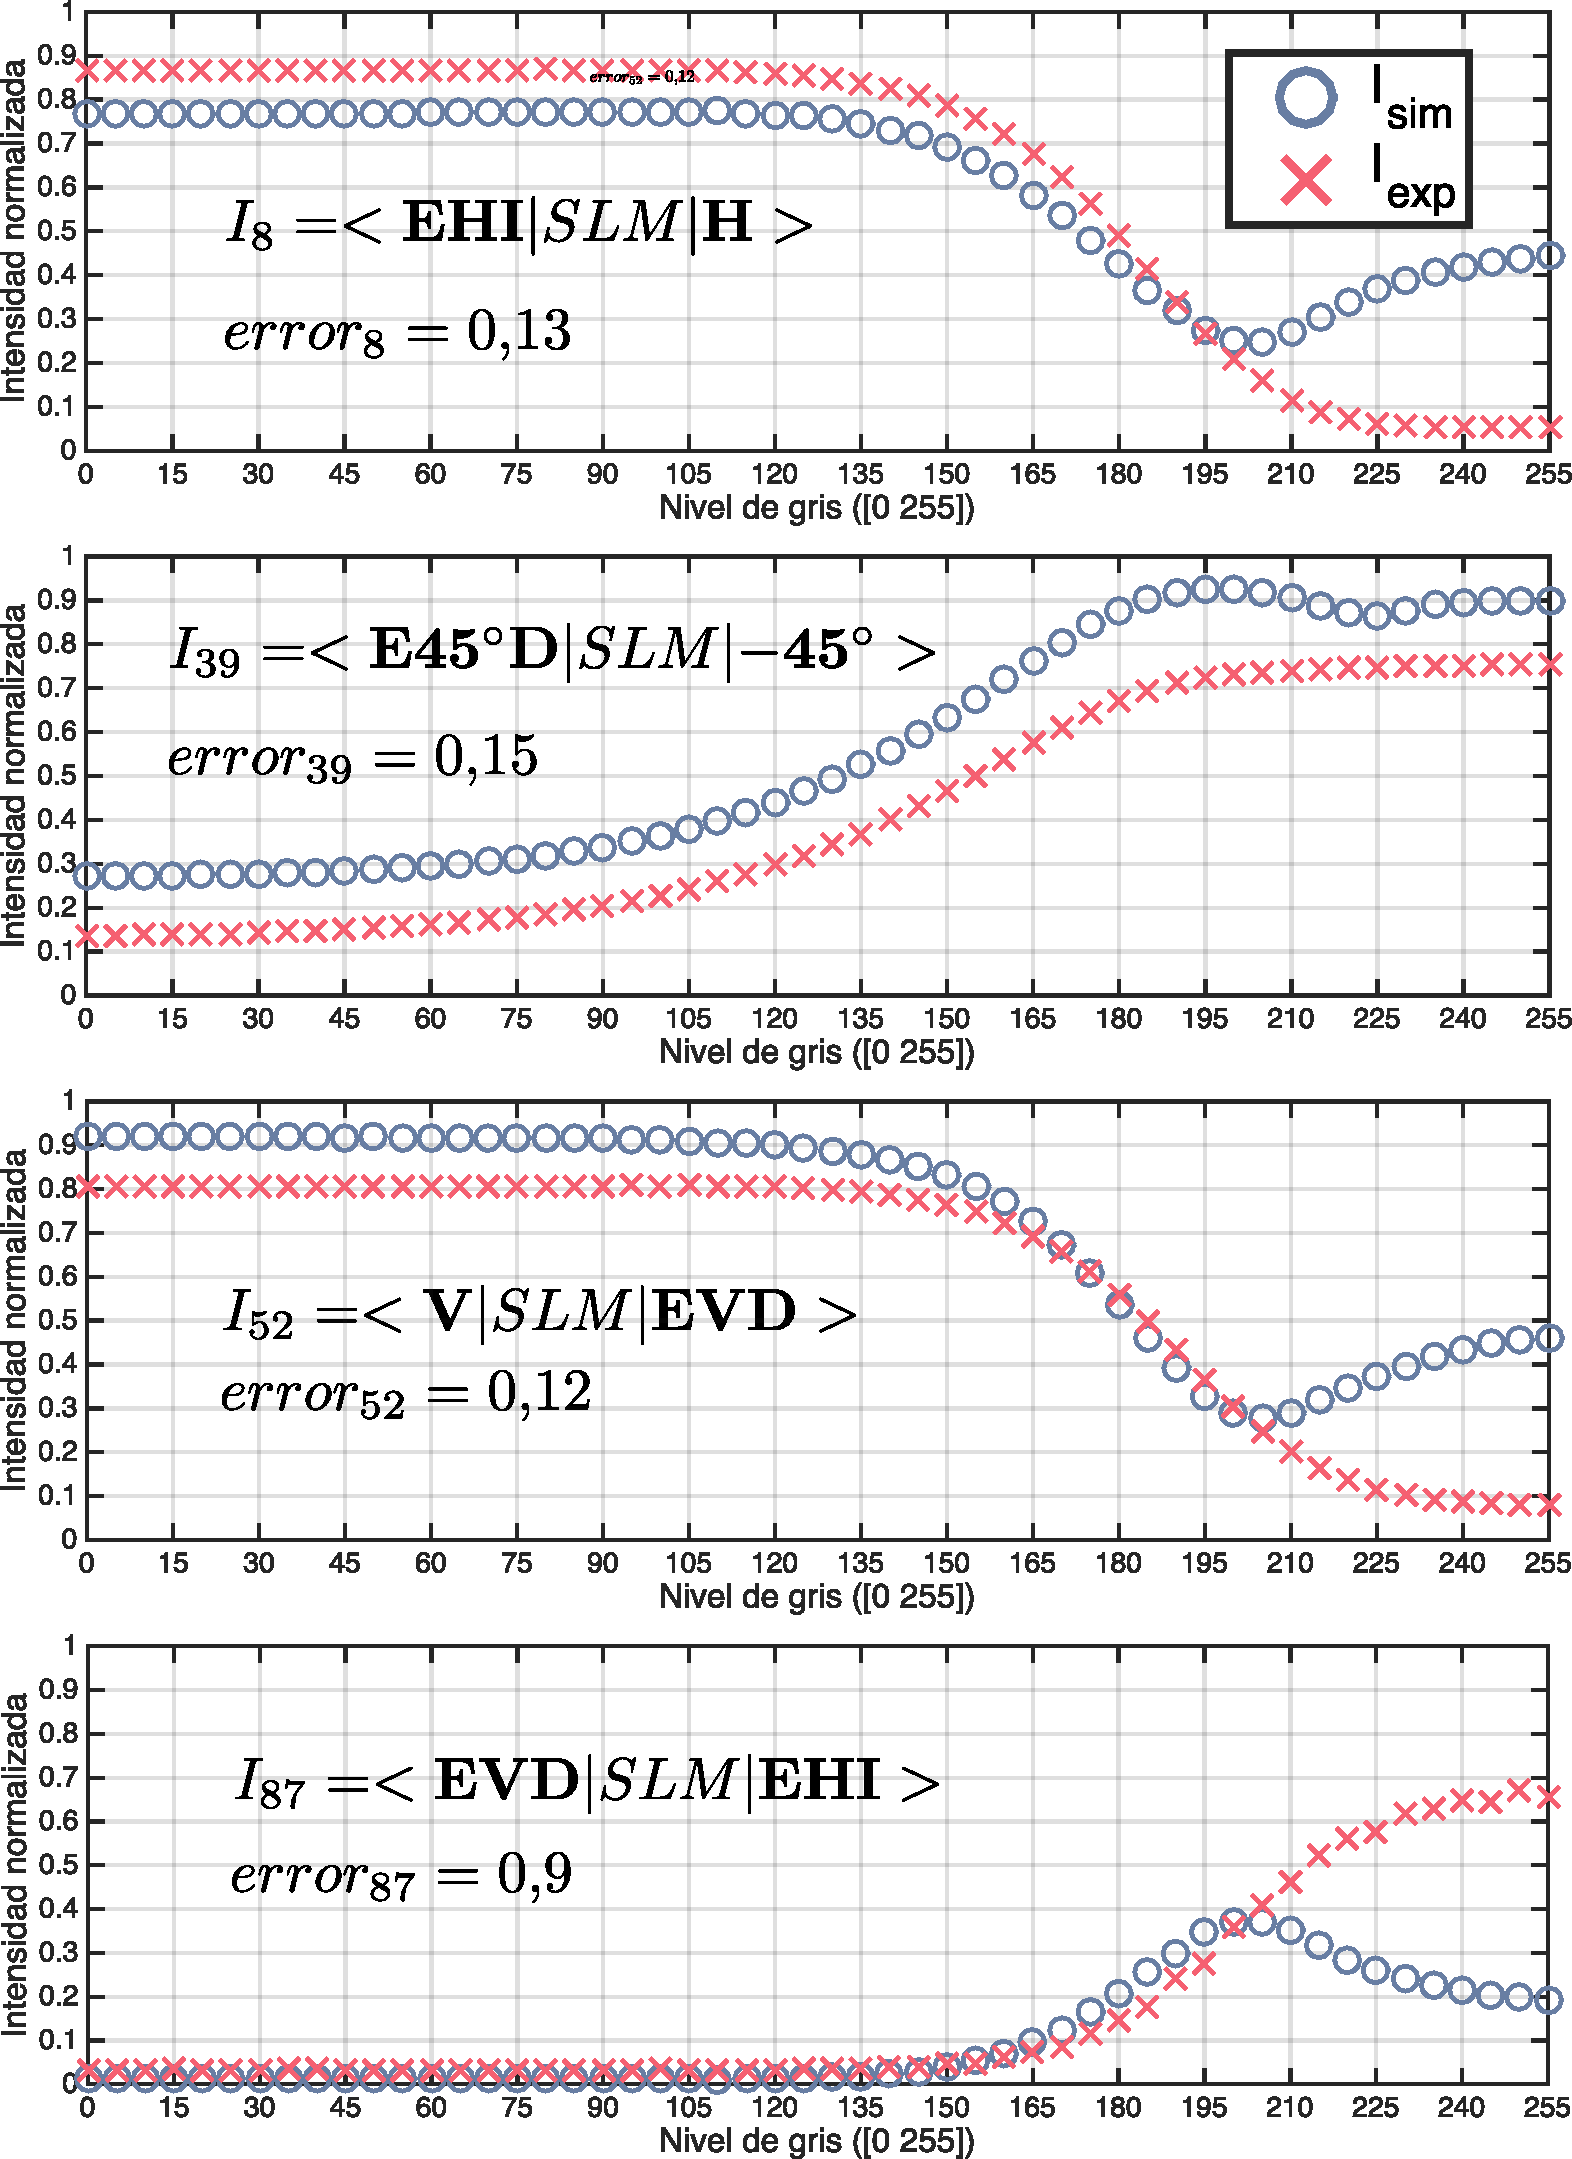
\includegraphics[scale=.5]{some_Ma_caracterization_results.pdf}
\caption[Curvas de modulación experimentales comparadas con las
simuladas usando el modelo obtenido con el método de Ma et al]{Curvas de modulación
  experimentales de 4 de las 100 medidas comparadas con sus
  equivalentes simuladas usando la matriz recuperada con el método de Ma et al.}
\label{fig:Ma_caracterization_results}
\end{figure}
Los resultados de la Fig. \ref{fig:Ma_caracterization_results} hacen
evidente que el método de Ma et al falla en reproducir el comportamiento del SLM
para algunos estados. Más aún, si se revisan las 100 medidas se observa que el
método sólo acierta a reproducir la modulación de los 12 estados $
[1,2,11,12,25,26,35,35,43,44,73,74]$ que están estrechamente ligados a
los estados usados para la construcción de las matrices. Observamos
que la divergencia del método se hace muy notoria a partir del nivel
de gris 200 y esto puede estar relacionado con el cambio de pendiente
que sufre la curva del parámetro $Y^2$ en la
Fig. \ref{fig:Our_Ma_X2Y2Z2W2} que posiblemente se debe a un cambio de
signo de $Y$. Creemos que este error está asociado con la
falta de un criterio para la selección de signos y que en vez de
adivinar signos hasta tener un modelo adecuado conviene proponer un
método de caracterización que no dependa explicitamente de $X^2$, $Y^2$, $Z^2$ y $W^2$.

% Con el fin de obtener un modelo más preciso, y que solucionara los
% vacíos del que hemos presentado, propusimos un método de
% caracterización basado en búsquedas numéricas de parámetros basándonos
% en rutinas de minimización. 

\section{Un método basado en minimización de parámetros}
Encontrar los números complejos $A$ y $B$ (o reales $X$, $Y$, $Z$,
$W$) necesarios para ensamblar la
matriz de Jones puede ser interpretado como un problema de
minimización desde el punto de vista de ingeniería inversa. Desde esta
perspectiva, se puede tratar el SLM realmente como una caja negra y
conservar sólo la condición de unicidad de la matriz
como restricción de la minimización.  
En primera medida, usamos el mismo conjunto de 6 medidas 
% polarimetría que requiere de
% plantear un conjunto de medidas que den la información suficiente
% sobre los cambios en polarización introducidos por el SLM. 
del método de caracterización 
% basados en un modelos de caja negra 
de \citetChGen{Ma2010}, que son también los estados de polarización
degenerados (lineales
$\mathbf{H}$, $\mathbf{V}$, $\mathbf{\pm 45^{\circ}}$ y circulares), que según la
teoría de polarización de Jones y de Stokes brindan la información suficiente para
caracterizar los cambios de polarización introducidos por un elemento
óptico \citepChGen{Collett2005}.
% Basandonos en el trabajo de Moreno, y con la convicción de que
% parametrizaban una variedad suficientemente diversa de situaciones
% escogimos las siguientes configuraciones de PSG y PSD para alimentar
% el algorítmo de ajuste.  
% \begin{align*}
% I_1 &= <\mathbf{V}|SLM|\mathbf{V}>& I_5 &=
%                                           <\mathbf{45^{\circ}}|SLM|\mathbf{45^{\circ}}>&I_9
%   &= <\mathbf{R}|SLM|\mathbf{R}>\\
% I_2 &= <\mathbf{H}|SLM|\mathbf{V}>&I_6 &=
%                                          <\mathbf{-45^{\circ}}|SLM|\mathbf{45^{\circ}}>&I_{10}
%   &= <\mathbf{L}|SLM|\mathbf{R}>\\
% I_3 &= <\mathbf{V}|SLM|\mathbf{H}>&I_7 &= <\mathbf{45^{\circ}}|SLM|\mathbf{-45^{\circ}}>&I_{11} &= <\mathbf{R}|SLM|\mathbf{L}>\\
% I_4 &= <\mathbf{H}|SLM|\mathbf{H}>&I_8 &=
%                                          <\mathbf{-45^{\circ}}|SLM|\mathbf{45^{\circ}}>&I_{12}
%   &= <\mathbf{L}|SLM|\mathbf{L}> 
% \end{align*}
% \begin{align*}
% I_1 &= |<\mathbf{V}|SLM|\mathbf{V}>|^2,& I_3 &=
%                                           |<\mathbf{45^{\circ}}|SLM|\mathbf{45^{\circ}}>|^2,&I_5
%   &= |<\mathbf{CD}|SLM|\mathbf{CD}>|^2,\\
% I_2 &= |<\mathbf{H}|SLM|\mathbf{V}>|^2,&I_4 &=
%                                          |<\mathbf{-45^{\circ}}|SLM|\mathbf{45^{\circ}}>|^2,&I_{6}
%   &= |<\mathbf{CI}|SLM|\mathbf{CD}>|^2.
% \end{align*}
Las curvas de modulación correspondientes a cada una de las medidas en
la notación de Ma y en notación la de la
Fig.~\ref{fig:braket_100_notation}, pueden verse en la Fig.~\ref{fig:six_input_measures}. 
\begin{figure}[h!]
\centering
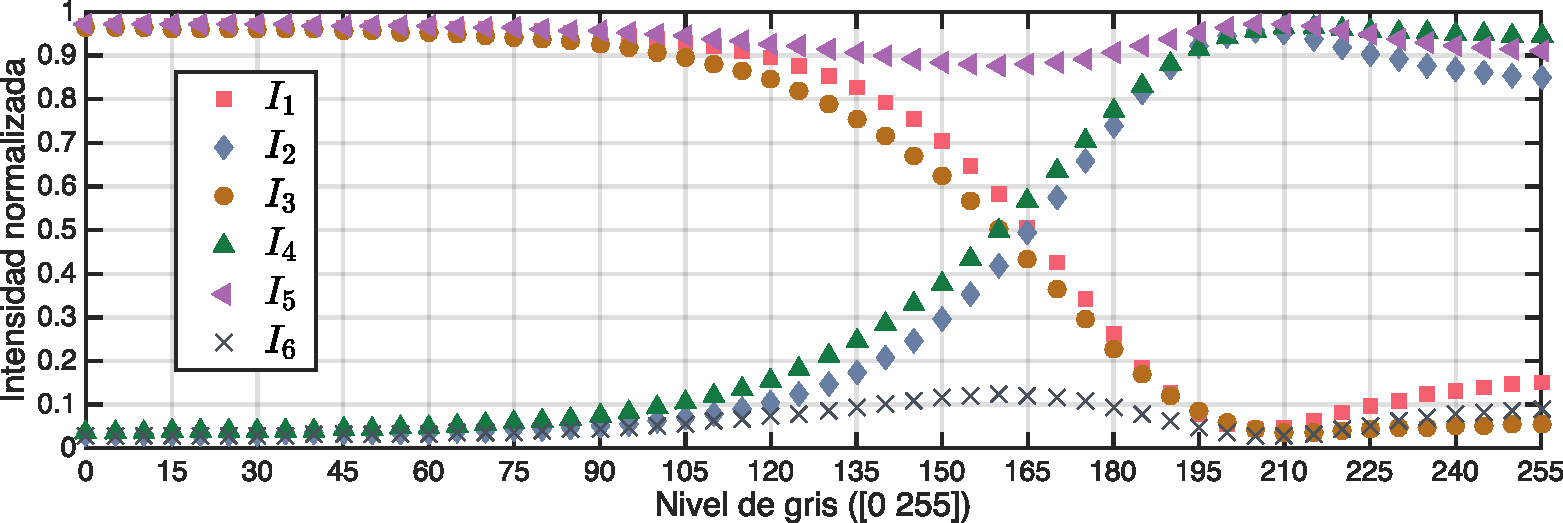
\includegraphics[scale=.55]{six_input_measures.pdf}
\caption[Curvas de modulación que sirven de entrada para el ajuste de
parámetros de la matriz de Jones del SLM]{Curvas de modulación que
  sirven de entrada para el ajuste de parámetros de la matriz de Jones
  del SLM. La leyenda indica la equivalencia entre las 6 curvas del
  método de Ma et al y la notación usada para las 100 medidas de comprobación. }
\label{fig:six_input_measures}
\end{figure}
Se puede observar que la modulación de amplitud es muy similar entre
polarizaciones lineales y que, como sería de esperarse, hay
complementariedad entre estados ortogonales.  Por otra parte, se
observa claramente que el SLM es cercano a ser transparente en un
amplio rango de niveles cuando se genera y detecta polarización
circular derecha, y opaco cuando se genera polarización circular
derecha y se detecta circular izquierda.
A continuación se describe la el funcional usado para la función de
minimización y la implementación del método. 
\subsection{Funcional a minimizar}
Una matriz de Jones que represente correctamente al SLM, encontrada por
métodos de minimización, debería en principio poder
emular al menos estas 6 medidas para lograr resultados tan buenos como
los del método de Ma et al. Nosotros planteamos un funcional a
minimizar ($\mathcal{L}$) que actúa como una medida de la similitud entre 
intensidades simuladas e intensidades adquiridas experimentalmente. El
funcional sirve como un criterio de selección para evaluar si los
parámetros propuestos ($(\mathbf{X,Y,Z,W})$) en alguna de las iteraciones de la rutina de
minimización son parámetros que reproduzcan las medidas
experimentales.  
\begin{equation}
\mathcal{L}(\mathbf{X,Y,Z,W}) = \sum_{ng=0}^{255}\sum_{i=1}^6 | I_{ng,i} -
|<\mathbf{J_{i}}|\mathbf{SLM_{ng}}|\mathbf{J_{i}}>|^2|^2.
\label{eq:ChGen_SLM_model_functional}  
\end{equation}
El funcional de la Eq. \ref{eq:ChGen_SLM_model_functional}  consiste en
la suma de las diferencias cuadradas entre intensidades para cada
nivel de gris ($n$) y para cada combinación de PSG y PSD ($i$). Los
argumentos del funcional son vectores que representan el conjunto de números
reales $X_n, Y_n, Z_n, W_n$ que componen a los elementos complejos $A$ y $B$
de la matriz de Jones del SLM (ver 
Eq. \ref{eq:general_jones_matrix}) para un $n$ dado,
\begin{align*}
\mathbf{X} &= \sum_{n=0}^{255}X_n,&\mathbf{Y} &= \sum_{n=0}^{255}Y_n,&\mathbf{Z} &= \sum_{n=0}^{255}Z_n,&\mathbf{W} &= \sum_{n=0}^{255}W_n.
\end{align*} 
El funcional \ref{eq:ChGen_SLM_model_functional}  puede ser minimizado
variando los 1024 ($256\times 4$) posibles valores 
de $X,Y,Z,W$ dentro del rango $-1:1$ en un algoritmo de
minimización. La minimización de los datos presentados en la
Fig. \ref{fig:six_input_measures} se llevo a cabo usando la función,\\
\hspace*{\fill}
\href{http://goo.gl/tv5Iyz}{\bf{scipy.optimize.fmin\_l\_bfgs\_b}}, \hspace*{\fill}\\ del
 paquete de calculo científico \href{http://goo.gl/fRhz8s}{\textbf{Scipy}} del
 lenguaje de programación \href{https://www.python.org}{\textbf{Python}}. Ésta
 función conocida como \href{http://en.wikipedia.org/wiki/Limited-memory\_BFGS}{\textbf{L-BFGS-B}} implementa una versión de memoria limitada del método quasi
 Newton conocido como Broyden-Fletcher-Goldfarb-Shano y permite
 la definición de condiciones de frontera sobre los argumentos de
 entrada.  
La implementación en el lenguaje Python de la función a minimizar se
muestra en la Fig. \ref{fig:SLM_functional},  
\begin{figure}
\begin{python}
def min_sq(x0,I_exp):
    """ Calculates squared differences for a minimization procedure.

    Given the experimental meassures of intensity and arbitrary values for 
    the parameters of an SLM Jones Matrix, this function gives a value to
    minimize. That value tells how close is the estimation of x, y, z, w 
    to the value that correctly models the SLM.

    :param x,y,z,w: Are a guess of real scalars that conform the Joung Matrix for the SLM.
    :param I_exp: Is a dictionary contanining intensities for every polarization state.
    """
    # brakets is a dictionary containing each pair of Jones vectors
    brakets = {1:translate_Ellipse_to_Jones([ 0,   0],      [0,0]),\
           2:translate_Ellipse_to_Jones([ pi/2,0],      [0,0]),\
           3:translate_Ellipse_to_Jones([ pi/4, 0],    [pi/4,0]),\
           4:translate_Ellipse_to_Jones([-pi/4, 0],    [pi/4,0]),\
           5:translate_Ellipse_to_Jones([pi/4,-pi/4],   [pi/4,-pi/4]),\
           6:translate_Ellipse_to_Jones([ -pi/4,pi/4],  [pi/4,-pi/4])}
    [x,y,z,w] = x0
    M = matrix([[ x + y*1j, z + w*1j],\
                [-z + w*1j, x - y*1j]])
    min_sum = 0
    I_sim = {}
    for i in range(1,nMeasures):
        Out, In = brakets[i]
        I_sim[i] = (In.H*M.H*Out * Out.H*M*In)
        min_sum += ((I_sim[i]-I_exp[i])**2)[0,0].real    
    return min_sum
\end{python}
\caption{Funcional a minimizar para el ajuste de parámetros basado en
  6 medidas de modulación de amplitud.}
\label{fig:SLM_functional}
\end{figure}
%\pagebreak
y la llamada a la función de minimización se hace como se muestra en la
Fig. \ref{fig:SLM_minimization}.
%cons = ({'type': 'eq', 'fun': lambda x:  x[0]**2+x[1]**2+x[2]**2+x[3]**2 - 1})
\begin{figure}
\begin{python}
bnds = ((-1, 1), (-1, 1),(-1, 1), (-1, 1))
x,y,z,w = [0.0001, 0.0001, -0.0001, -0.0001] 
res_f = {}
for g in range(52):
    I_exp = I_list[g]
    res = fmin_l_bfgs_b(min_sq, [ x,y,z,w], fprime = None,\
                         approx_grad = 1,args = (I_exp,brakets),\
                         pgtol=1e-05, bounds =bnds)
    x,y,z,w = res[0]
    res_f[g] = res[0]
    print(res[0])
\end{python}
\caption{Condiciones de frontera, argumentos iniciales y llamado de la
función de minimización (fmin\_l\_bfgs\_b) para cada nivel de gris.}
\label{fig:SLM_minimization}
\end{figure}
En este caso usamos un valor semilla para los valores de entrada muy
cercano a cero, utilizamos la opción de aproximación del gradiente
por medio de diferencias finitas y definimos la tolerancia de
convergencia como criterio de parada cuando el valor del funcional no
cambie menos de $1e^{-5}$. Los detalles sobre las variables,
preprocesamiento, y los resultados se han subido a internét en un
repositorio de GitHub y se pueden observar en la siguiente página
web:\\
\hspace*{\fill} \href{http://goo.gl/FLIGE0}{\textbf{http://goo.gl/FLIGE0}}.\hspace*{\fill} \\
%\hspace*{\fill} \href{http://goo.gl/QQtcQX}{\textbf{http://goo.gl/QQtcQX}}.\hspace*{\fill} \\
En la figura \ref{fig:xyzw} se presentan los valores de $X,Y,Z,W$ obtenidos luego de
ejecutar la minimización. 
\begin{figure}[h!]
\centering
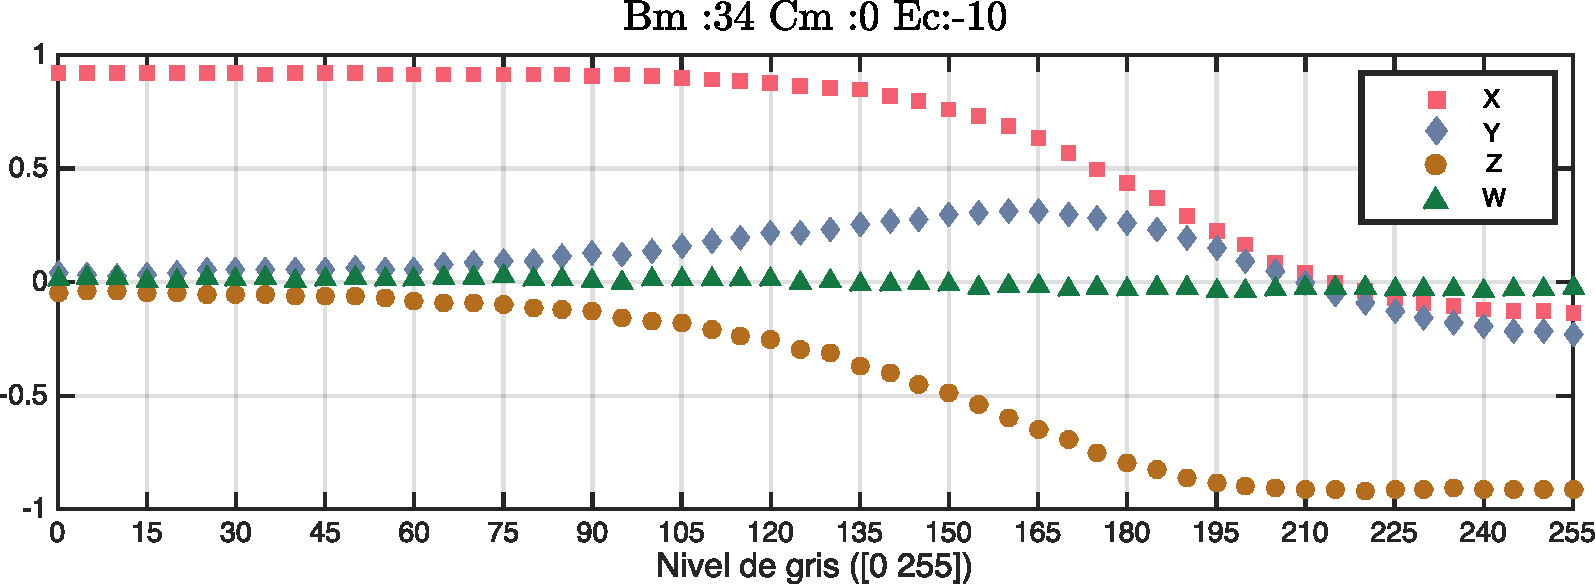
\includegraphics[scale=.55]{xyzw.pdf}
\caption[Parametros reales que conforman la matriz de Jones del SLM
encontrados por minimización con 6 medidas]{Parametros reales que
  conforman la matriz de Jones del SLM encontrados por medio de
  minimización con 100 entradas.} 
\label{fig:xyzw}
\end{figure}
Contrario a lo que pensábamos, resultó que aún cuando el método de
minimización se basa directamente en los valores $X,Y,Z$, y $W$, y no
en sus cuadrados, los resultados son casi idénticos a los que
obtuvimos en la sección anterior con el método de Ma et~al. Las curvas
de los parámetros del modulador siguen la misma tendencia y producen
los mismos valores de intensidad en las simulaciones. Las 4 medidas
con estados elípticos que se  
presentaron en la Fig. \ref{fig:Ma_caracterization_results} se
repitieron para el nuevo método y se presentan junto con el valor del
error relativo promedio porcentual en la
Fig. \ref{fig:6m_caracterization_results}. 
%\newpage
\begin{figure}[h!]
\centering
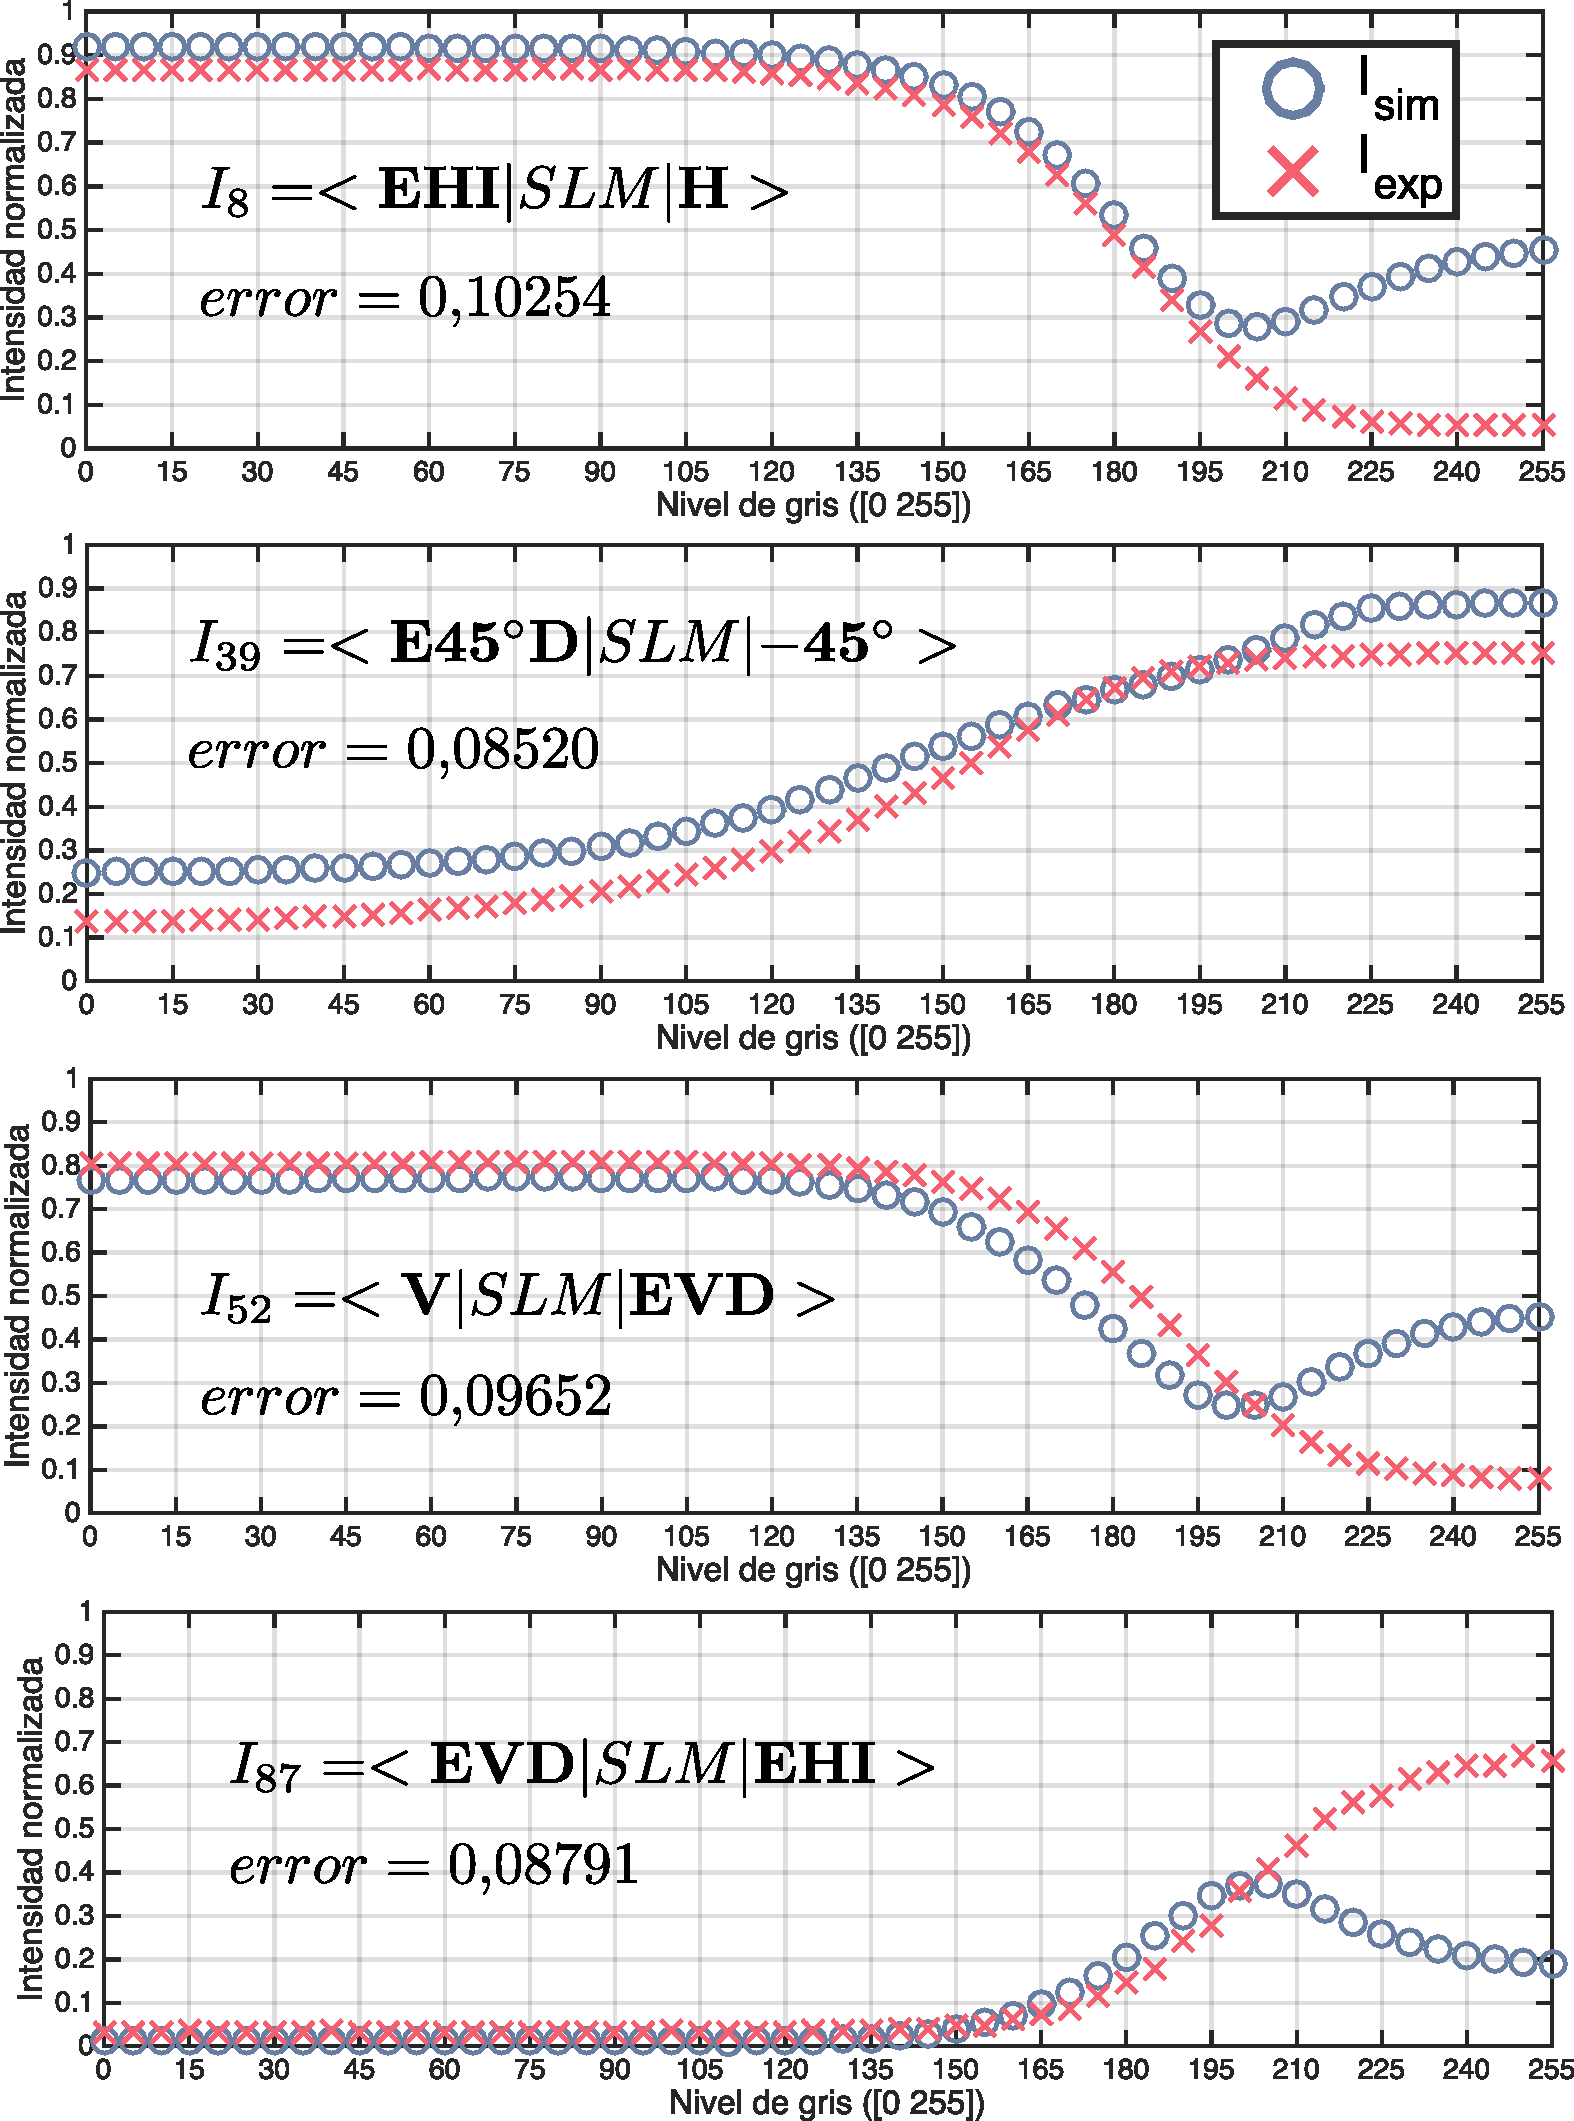
\includegraphics[scale=.5]{some_6min_caracterization_results.pdf}
\caption[Curvas de modulación experimentales comparadas con las
simuladas usando el modelo obtenido con el método de minimización de 6
medidas]{Curvas de modulación
  experimentales, y error de 4 de las 100 medidas comparadas con sus
  equivalentes simuladas usando la matriz recuperada con el método de
  minimización con 6 medidas.}
\label{fig:6m_caracterization_results}
\end{figure}
El error en las 6 medidas usadas como entrada es en este caso menor a
$2\times10^{-4}$, y el error absoluto global es de $error_g
=0.077673$, que es un poco menor que el anterior. Sin embargo, sigue ocurriendo que la exactitud se pierde a partir del
nivel de gris 200 en la mayoría de los estados. Es decir, que con estas medidas como entrada
nuestro método es tan bueno como el de la literatura pero no
significativamente mejor.
\pagebreak
\subsection{Una ampliación de la función de minimización}
El funcional de minimización puede ser modificado
fácilmente para incluir como valores de entrada cuantos BraKet's
distintos se deseen siempre y cuando se conozcan los vectores de Jones 
correspondientes al PSG y PSD de cada uno.   
Siguiendo la idea de utilizar la información extra de la que disponemos, modificamos la
función para recibir no 6 sino 100 estados de entrada y 
ejecutamos de nuevo el algoritmo de minimización. Los parámetros de
Jones para cada nivel de gris del método de minimización extendido
se presentan en la Fig. \ref{fig:xyzw_100}, e inmediatamente se puede observar un
cambio importante en el comportamiento de las curvas $X$, $Y$, y $W$
en comparación con las figuras \ref{fig:Ma_and_our_XYZW} y
\ref{fig:xyzw}. 
\begin{figure}[h!]
\centering
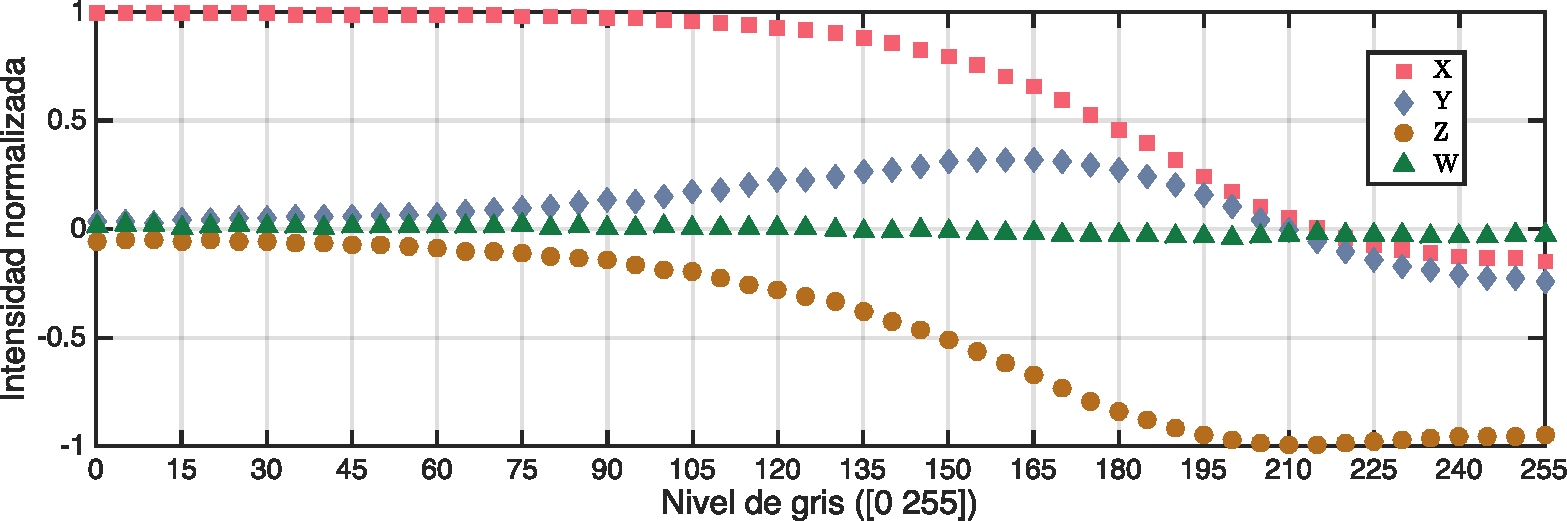
\includegraphics[scale=.55]{xyzw_100.pdf}
\caption[Parametros reales que conforman la matriz de Jones del
SLM encontrados por minimización con 100 medidas]{Parametros reales
  que conforman la matriz de Jones del SLM 
  encontrados por medio de minimización con 100 entradas.}
\label{fig:xyzw_100}
\end{figure}
Como se había supuesto, se puede ver que los valores de $Y$
para los niveles más allá del 200 son negativos, y que $W$ es
virtualente cero para todo el rango de niveles. Además, se observa que
$X$ también adquiere valores negativos para niveles de gris por encima
de 200.   
Con respecto a las medidas de intensidad, se obtuvo una mejoría cuantitativa
significativa con un error absoluto global de $error_g= 0.024162$ que
es 3.5 veces menor que el obtenido con el método de Ma et al. No
obstante, la calidad de la solución se hace más evidente cuando se
comparan los resultados cualitativamente, y se observa que los cambios
de dirección que surgían a partir del nivel de gris 200 han
desaparecido. Como antes, se presentan 4 de las medidas con estados
elípticos en la Fig. \ref{fig:100m_caracterization_results} y los
resultados completos han sido 
alojados en \href{http://goo.gl/kZjVGU}{\textbf{http://goo.gl/kZjVGU}}.
\begin{figure}[h!]
\centering
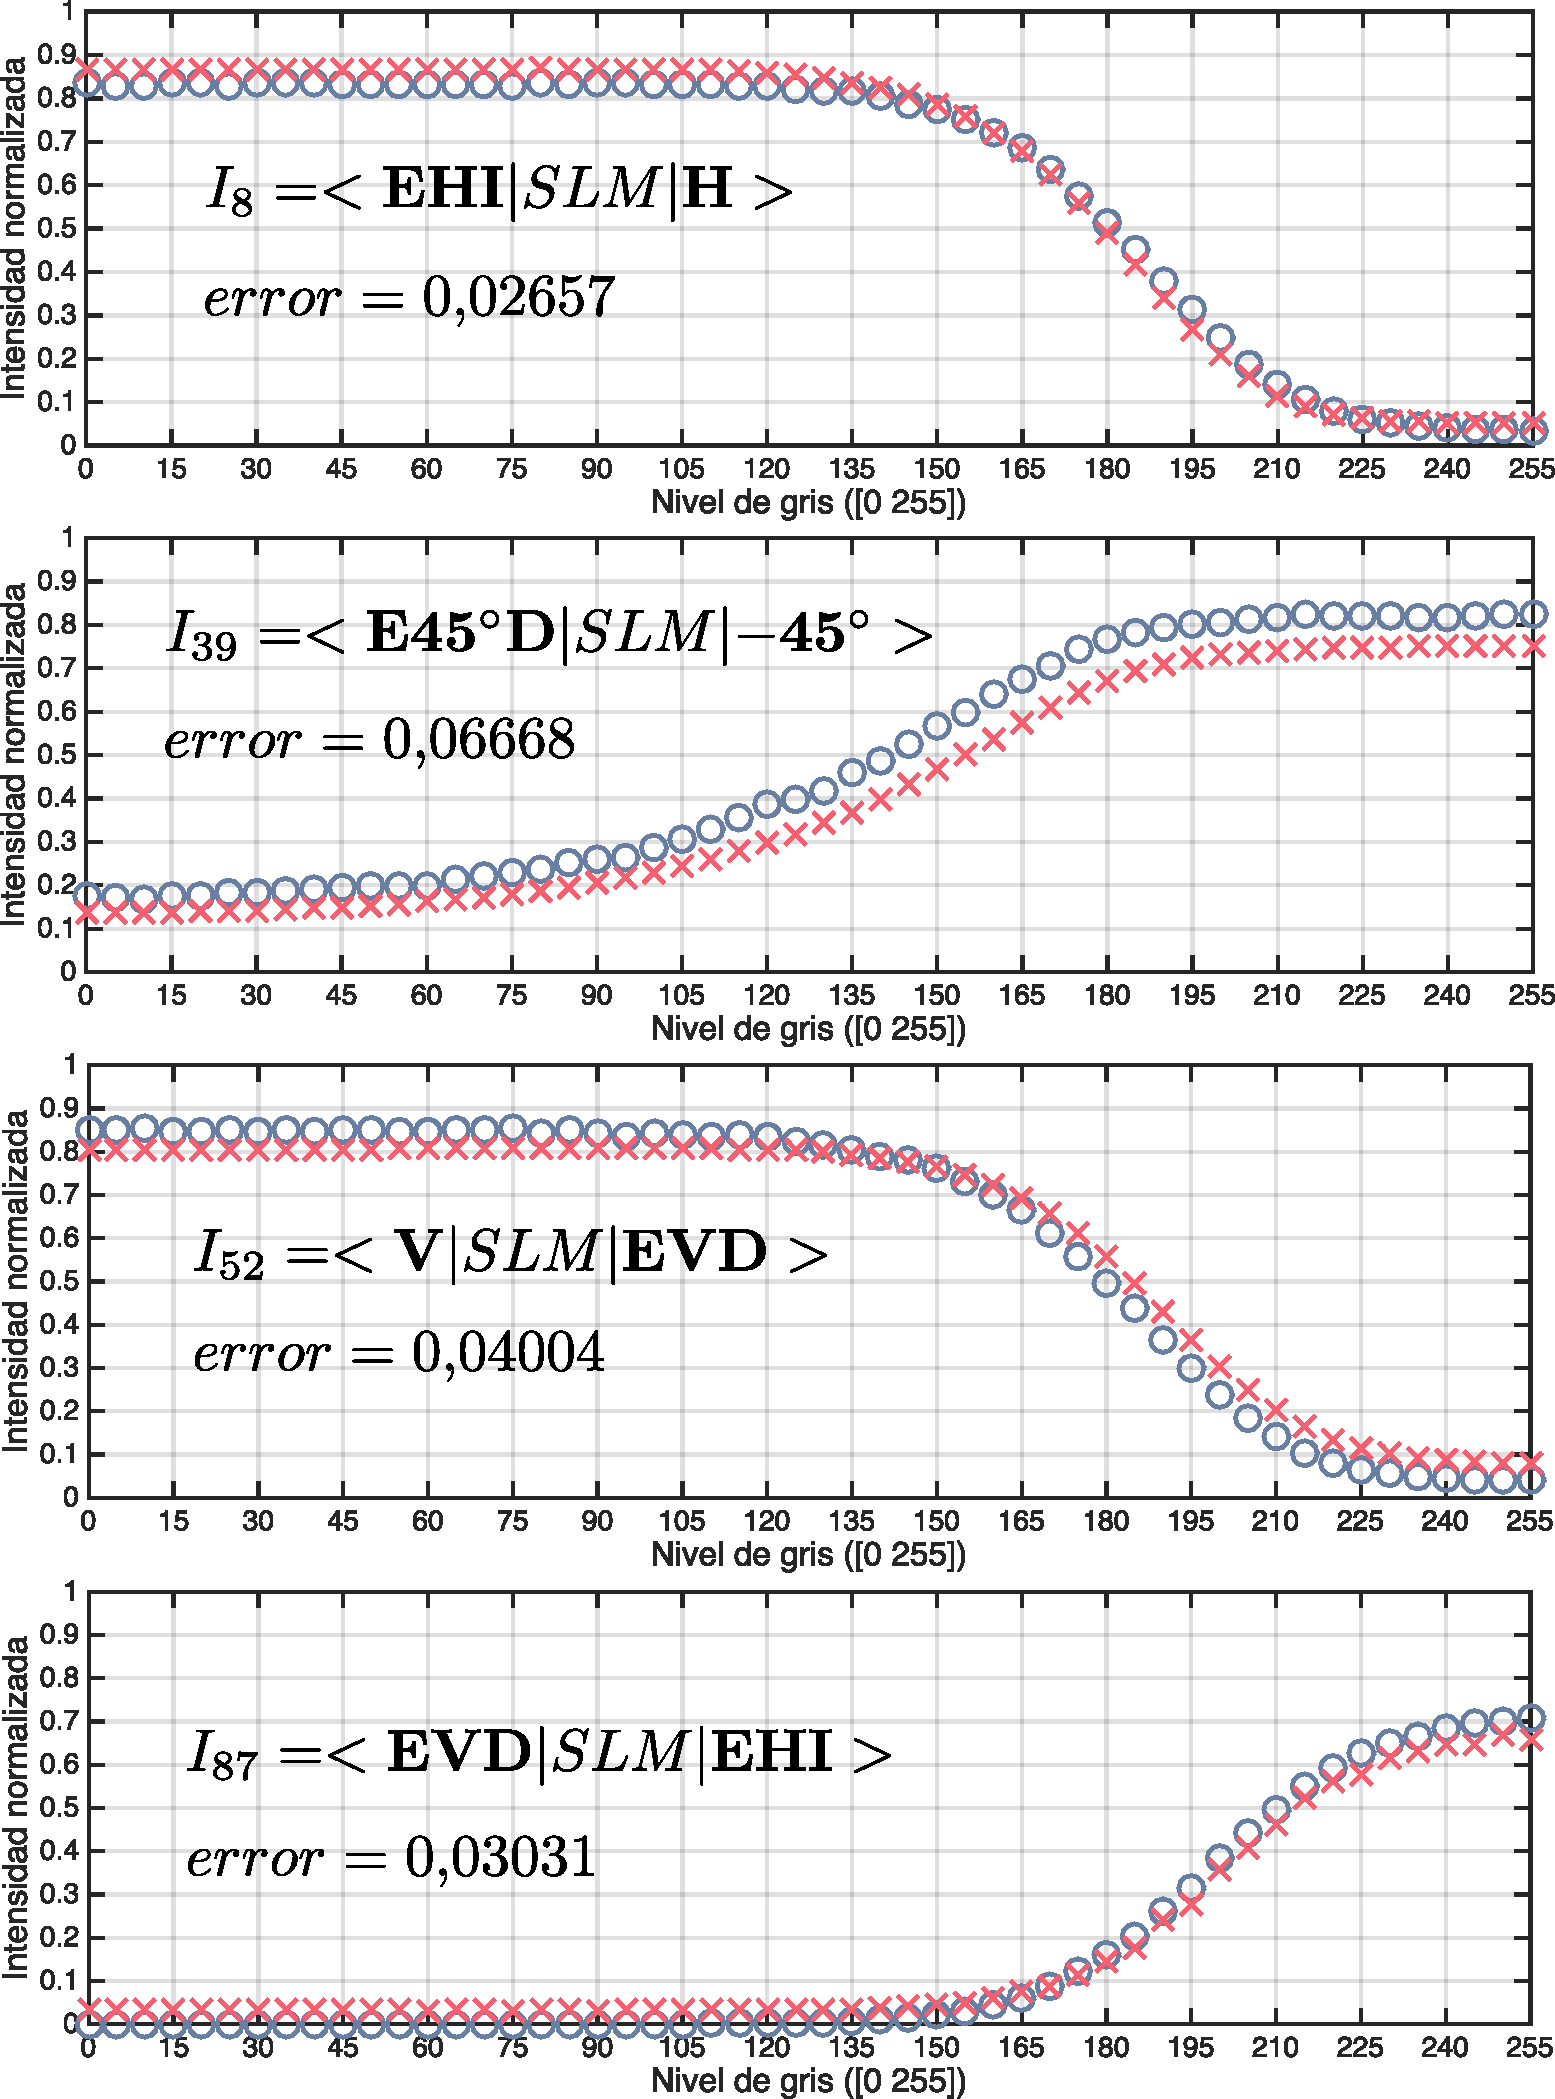
\includegraphics[scale=.5]{some_100_caracterization_results.pdf}
\caption[Curvas de modulación experimentales comparadas con las
simuladas usando el modelo obtenido con el método de minimización de 100
medidas]{Curvas de modulación
  experimentales, y error de 4 de las 100 medidas comparadas con sus
  equivalentes simuladas usando la matriz recuperada con el método de
  minimización con 100 medidas de entrada.}
\label{fig:100m_caracterization_results}
\end{figure}
En conclusión, Lo que muestran los resultados es que se logró una muy buena aproximación, y que el modelo de la matriz de Jones del SLM efectivamente
reproduce la modulación de amplitud del elemento real. 
\subsubsection{Instrumento para la automatización del proceso de
  medida.}
\label{sec:instrumento}
Ahora bien, cualquiera que haya tenido experiencia con la
caracterización de SLMs se sorprenderá por la cantidad de medidas que
hemos hecho. La toma de cientos de medidas y todo el proceso de
aprendizaje sobre la polarimetría fue posible sólo
porque usamos un instrumento mecatrónico desarrollado por nosotros
antes y durante este trabajo de grado. El Instrumento se muestra en la
Fig. \ref{fig:montaje_real_polarimetro} y consiste en
cuatro rotadores ópticos motorizados manipulados por un computador a
traves de la tarjeta de prototipado rápido
\href{http://www.arduino.cc/en/Main/ArduinoBoardLeonardo}{\bf{Arduino Leonardo}}. 
\begin{figure}[h!]
\centering
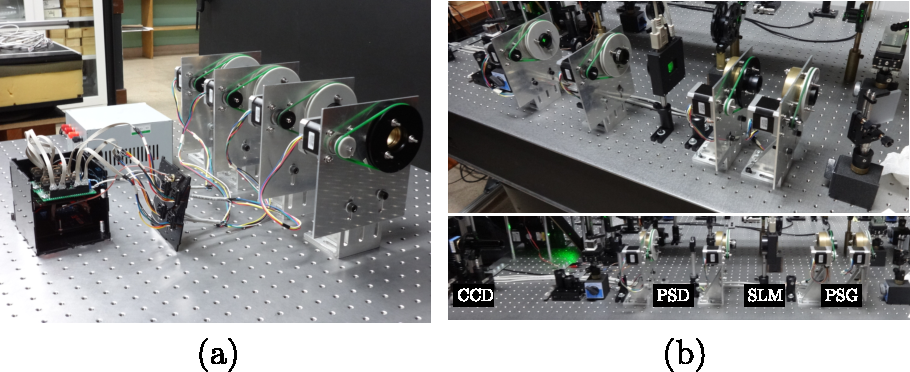
\includegraphics[scale=.96]{montaje_real_polarimetro.pdf}
\caption[Hardware del instrumento de polarimetría y montaje
experimental ]{(a) Hardware del instrumento de polarimetría que se
  compone de 4 rotadores de elementos ópticos, una fuente de voltaje,
  y una caja de circuitos electrónicos en donde está el Arduino y la
  electrónica de potencia. (b) Montaje experimental correspondiente a
  la implementación de la Fig. \ref{fig:PSG_PSD}. }
\label{fig:montaje_real_polarimetro}
\end{figure}
 La interfaz de usuario del instrumento para toma de medidas y
calibración de motores fue programada como un
instrumento virtual del entorno de programación gráfica LabView, y los
comandos de movimiento para los motores son enviados al Arduino a
través de una librería de comunicación serial implementada en Python.
Las componentes mecánicas y electrónicas del instrumento se describen a profundidad en el
apéndice \ref{AppendixA}, y los programas de interfáz de usuario y
comunicación serial se describen el apéndice B.
El proceso de toma de cientos de medidas que a una persona podría llevarle varios
días de trabajo se hace con la interfaz en cuestión de una o dos horas
sin necesidad de supervisión.    
\pagebreak
%\subsection{Medida de la modulación de fase}
\section{Medida de la modulación de fase}
% El proceso de caracterización del SLM no queda completo sin antes
% comprobar que el modelo puede predecir modulaciones de fase. 
El paso siguiente en la caracterización del SLM consiste en medir la
modulación de fase y comprobar si la matriz de Jones encontrada es
capaz de predecir el comportamiento de este SLM. 
La fase del frente de onda se midió usando el interferómetro
\href{http://en.wikipedia.org/wiki/Mach–Zehnder_interferometer}{\bf{Mach–Zehnder}}
de la Fig. \ref{fig:mach_zehnder}. 
\begin{figure}[h!]
\centering
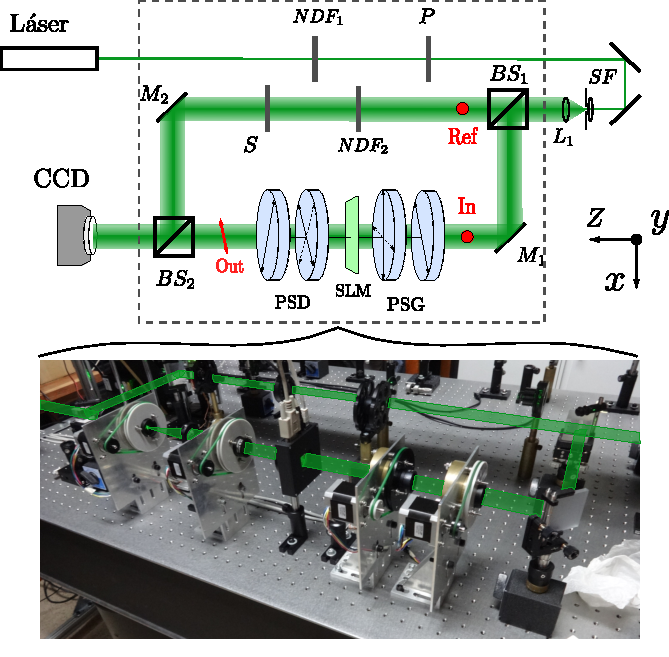
\includegraphics[scale=1.1]{mach_zehnder.pdf}
\caption[Interferómetro Mach-Zehnder para caracterización de curvas de
modulación de fase]{Interferómetro Mach-Zehnder para caracterización de curvas de
modulación de fase. }
\label{fig:mach_zehnder}
\end{figure}
En este montaje la fuente de iluminación es un láser de estado sólido
de diodo bombeado (DPSS) de longitud de onda 532nm y potencia nominal
50mW. El haz pasa por un filtro de densidad neutra ($NDF_1$) que sirve como
atenuador, y luego por un polarizador (P) de recubrimiento de
nanopartículas que garantiza una polarización lineal vertical con
relación  10.000:1. Este polarizador es usado porque el estado de
polarización a la salida del diodo láser es ligeramente elíptica y no
está perfectamente alineada con la vertical de la mesa óptica. 
Luego de ser redireccionado, el haz es filtrado, expandido y colimado
por medio de un filtro espacial (SF) en combinación con una lente
($L_1$). Una vez colimado, el haz pasa por un cubo divisor de haz no
polarizador ($BS_1$) que lo divide en un haz de referencia en la parte
superior y uno objeto en la parte inferior que ilumina
al SLM. El haz de entrada es reflejado en el espejo de primera
superficie $M_1$ y pasa a través del PSG, el SLM, y el PSD para luego
reencontrarse con el haz de referencia en un segundo cubo ($BS_2$) y
continuar su camino hasta la cámara CCD. A diferencia del haz objeto,
el haz de referencia sólo pasa por un segundo NDF que sirve para
compensar la relación entre intensidades de los dos haces. El elemento
$S$ es un obturador que se controla desde el computador y sirve para cambiar
del modo de medida de modulación de amplitud a modulación de fase.  

Al haber recorrido un camino que contiene elementos polarizadores y
birrefringentes, el haz objeto sufre cambios en su fase y en su estado
de polarización. Estos cambios se ven reflejados en la posición y
contraste de las franjas de los interferogramas registrados por la
cámara. En la figura \ref{fig:fringes} se pueden observar dos
interferogramas que se han tomado cuando a la salida del PSD hay (a)
un estado vertical, y (b) un estado horizontal.  
\begin{figure}[h!]
\centering
\includegraphics[scale=.5]{fringes.pdf}
\caption[Interferogramas obtenidos en el montaje experimental para
caracterización de modulación de fase]{Interferogramas obtenidos en el montaje experimental para
caracterización de modulación de fase. (a) Franjas de interferencia
cuando la polarización en los dos brazos es igual, y (b) cuando son
estados ortogonales.}
\label{fig:fringes}
\end{figure}

La caracterización de las curvas de modulación de amplitud está
asociada al cambio de contraste, y la modulación de fase es
proporcional al desplazamiento de las franjas. Un cambio de fase de
$\pi$ radianes hace que las franjas se desplazan hasta un punto en el
cual las que eran brillantes son ahora oscuras, y
viseversa. Caracterizar la modulación consiste en medir los 
desplazamientos de las franjas para cada nivel de gris de la pantalla
del SLM, y dado que cualquier vibración puede mover las franjas es
preferible capturar simultaneamente imágenes con las franjas en una
posición de referencia e imagenes con franjas 
desplazadas. Para ello, varios autores como \citetChGen{Moreno2003} y
\citetChGen{Ma2010} han proyectado al SLM una máscara con dos
secciones rectangulares, una con un nivel de gris constante (255) y
otra en la que el nivel de gris varía de 0 a 255. La máscara usada y
el interferograma resultante se muestran en la Fig. \ref{fig:split}.  
\begin{figure}[h!]
\centering
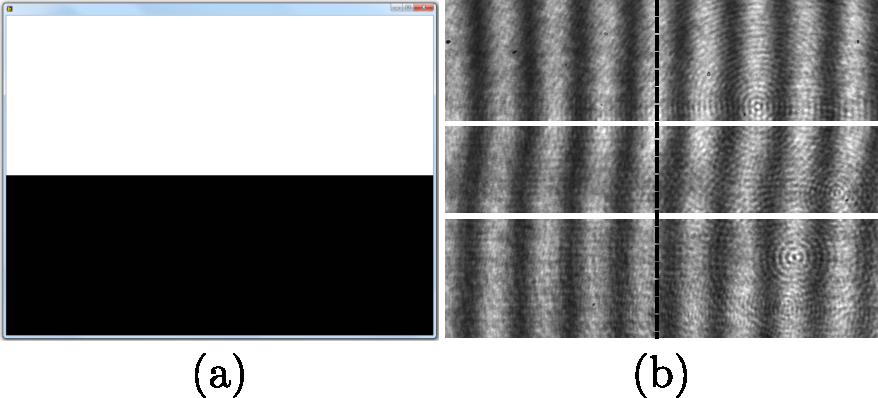
\includegraphics[scale=1]{split.pdf}
\caption[Máscara dividida e interferograma obtenido para
caracterización de modulación de fase]{(a) Máscara dividida y (b)
  interferograma registrado para
caracterización de modulación de fase. En esta combinación de PSG y
PSD se logró una modulación de aproximadamente $\pi/2$ que se puede
identificar con la línea de referencia punteada. La linea roja indica
que esa parte del interferograma se desecha.}
\label{fig:split}
\end{figure}

El interferograma de la Fig. \ref{fig:split}(b) se descompone en 3
imágenes, la imagen central se desecha, pues presenta un efecto de
borde indeseado que resulta de la difracción producida por el escalón
entre un nivel de gris y otro. Las imágenes superior e inferior corresponden a las franjas
de referencia y desplazadas respectivamente, y se conservan para
extraer la fase entre ellas. 
Para visualizar mejor las crestas
promediamos el valor de las primeras y últimas 100 filas y generamos
dos curvas en 1D de la intensidad normalizada por píxel como se
observa en la Fig. \ref{fig:fringes_plot}.  
\begin{figure}[h!]
\centering
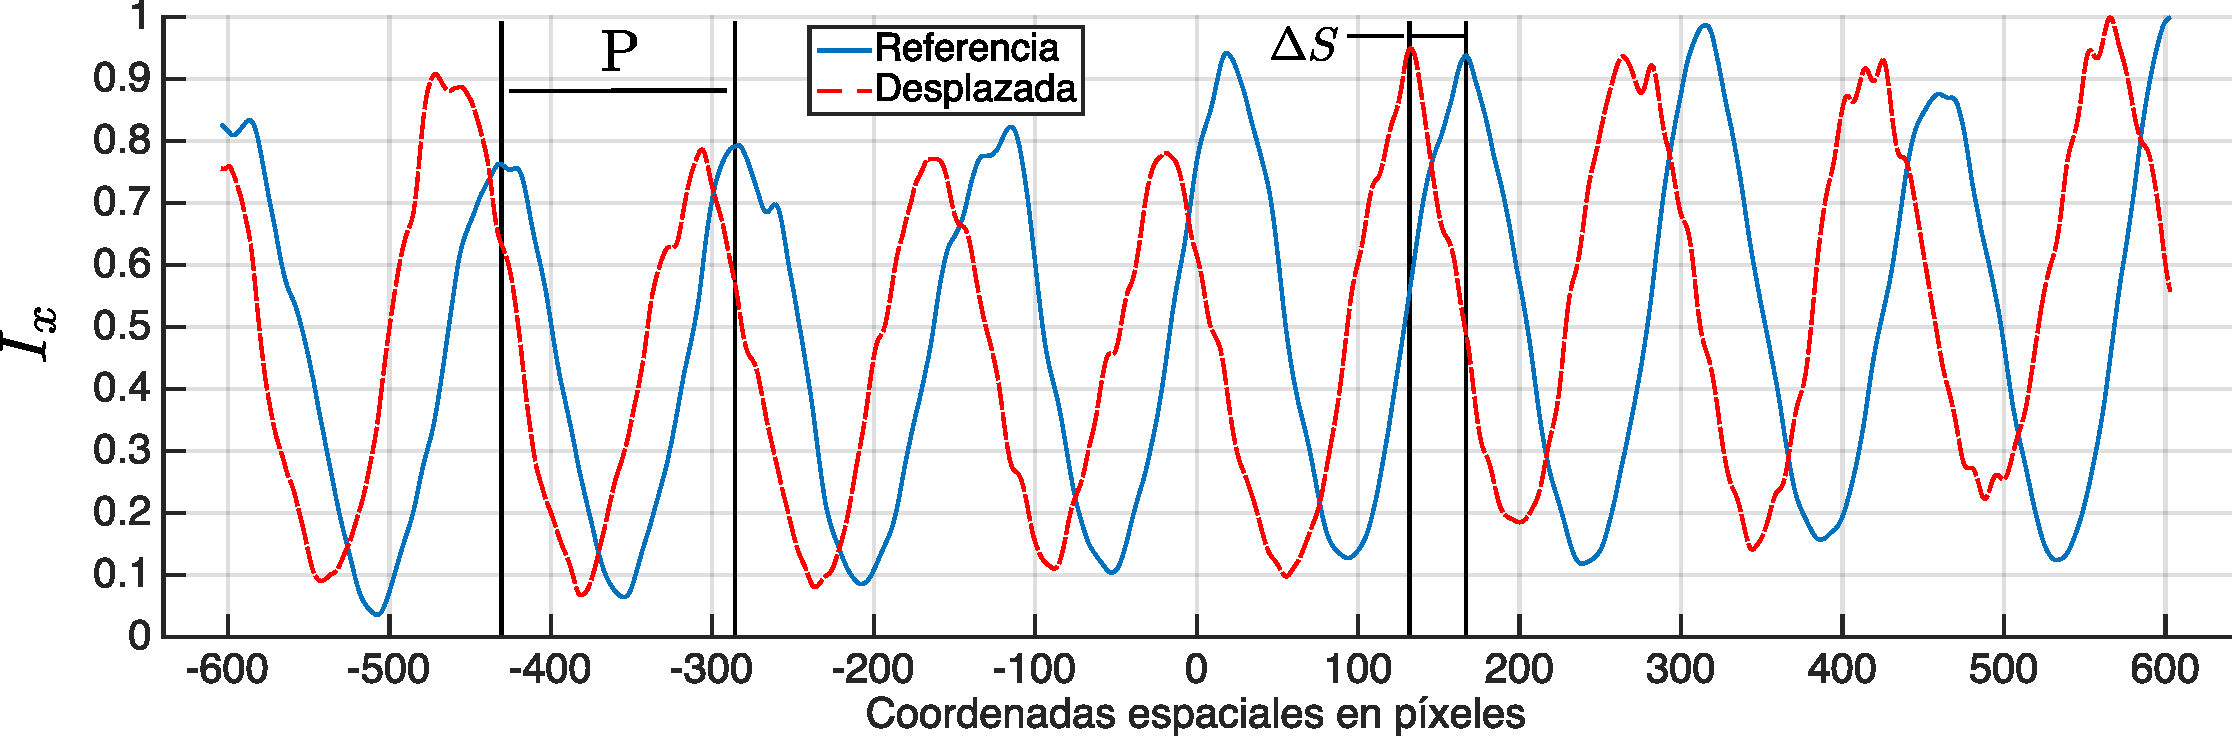
\includegraphics[scale=0.4]{fringes_plot_edited.pdf}
\caption[Patrones de interferencia 1D de interferogramas con y sin
desfase]{Patrones de interferencia 1D suavizados de los interferogramas con y sin
  desfase de la Fig. \ref{fig:split}. La imagen original tiene 1208
  píxeles y se tomó la mitad como cero.}
\label{fig:fringes_plot}
\end{figure}
La diferencia de fase $\Delta\phi$ puede ser extraída de los
interferogramas midiendo el periodo (P) y la distancia entre crestas ($\Delta S$) de la imagen de
referencia y la imagen desplazada haciendo el siguiente cálculo \citepChGen{Ma2010},
$$\Delta\phi = 2\pi \Delta S/P.$$
%De los datos en esta representación, se puede extraer la diferencia de
%fase $\Delta \phi$ a partir del periodo ($P$) sabiendo que $$\Delta
Extraer la fase de esta forma resulta bastante directo e intuitivo,
pero se aprovecha muy poca información de la señal y se pierde
precisión en comparación con otras alternativas. Además, este método resulta dificil de
programar en forma de un algorítmo. 

Otra forma de extraer la fase consiste en aplicar una \textbf{Transformada de
Fourier} (FT) a las señales e identificar los picos correspondientes a
la función seno o coseno asociada al patron de interferencia. La fase
de cada interferograma es la fase o ángulo del número complejo 
correspondiente al mayor pico de la FT una vez se ha filtrado el delta
de Dirac central correspondiente a la FT de la intensidad de fondo.  
Los picos se pueden identificar calculando el valor absoluto de la FT de
la señal y buscando el elemento más grande. La representación gráfica
de la FT se ilustra en la Fig. \ref{fig:fringes_f} con respecto a las
coordenadas de frecuencia espacial, y se observa claramente que se ha
filtrado el pico central y que la información de la FT se encuentra
alrededor de los picos en las frecuencias  8 y -8. Nosotros adaptamos
una implementación en Matlab de este método que fue inicialmente
propuesta para esta aplicación por el profesor Alberto Lencina del Centro de
Investigaciones Ópticas de Argentina. En la figura \ref{fig:fourier_script}, se muestra un
pequeño script que ilustra cómo se haría el cálculo de la fase del
interferograma de referencia.     
\begin{figure}[H]
\centering
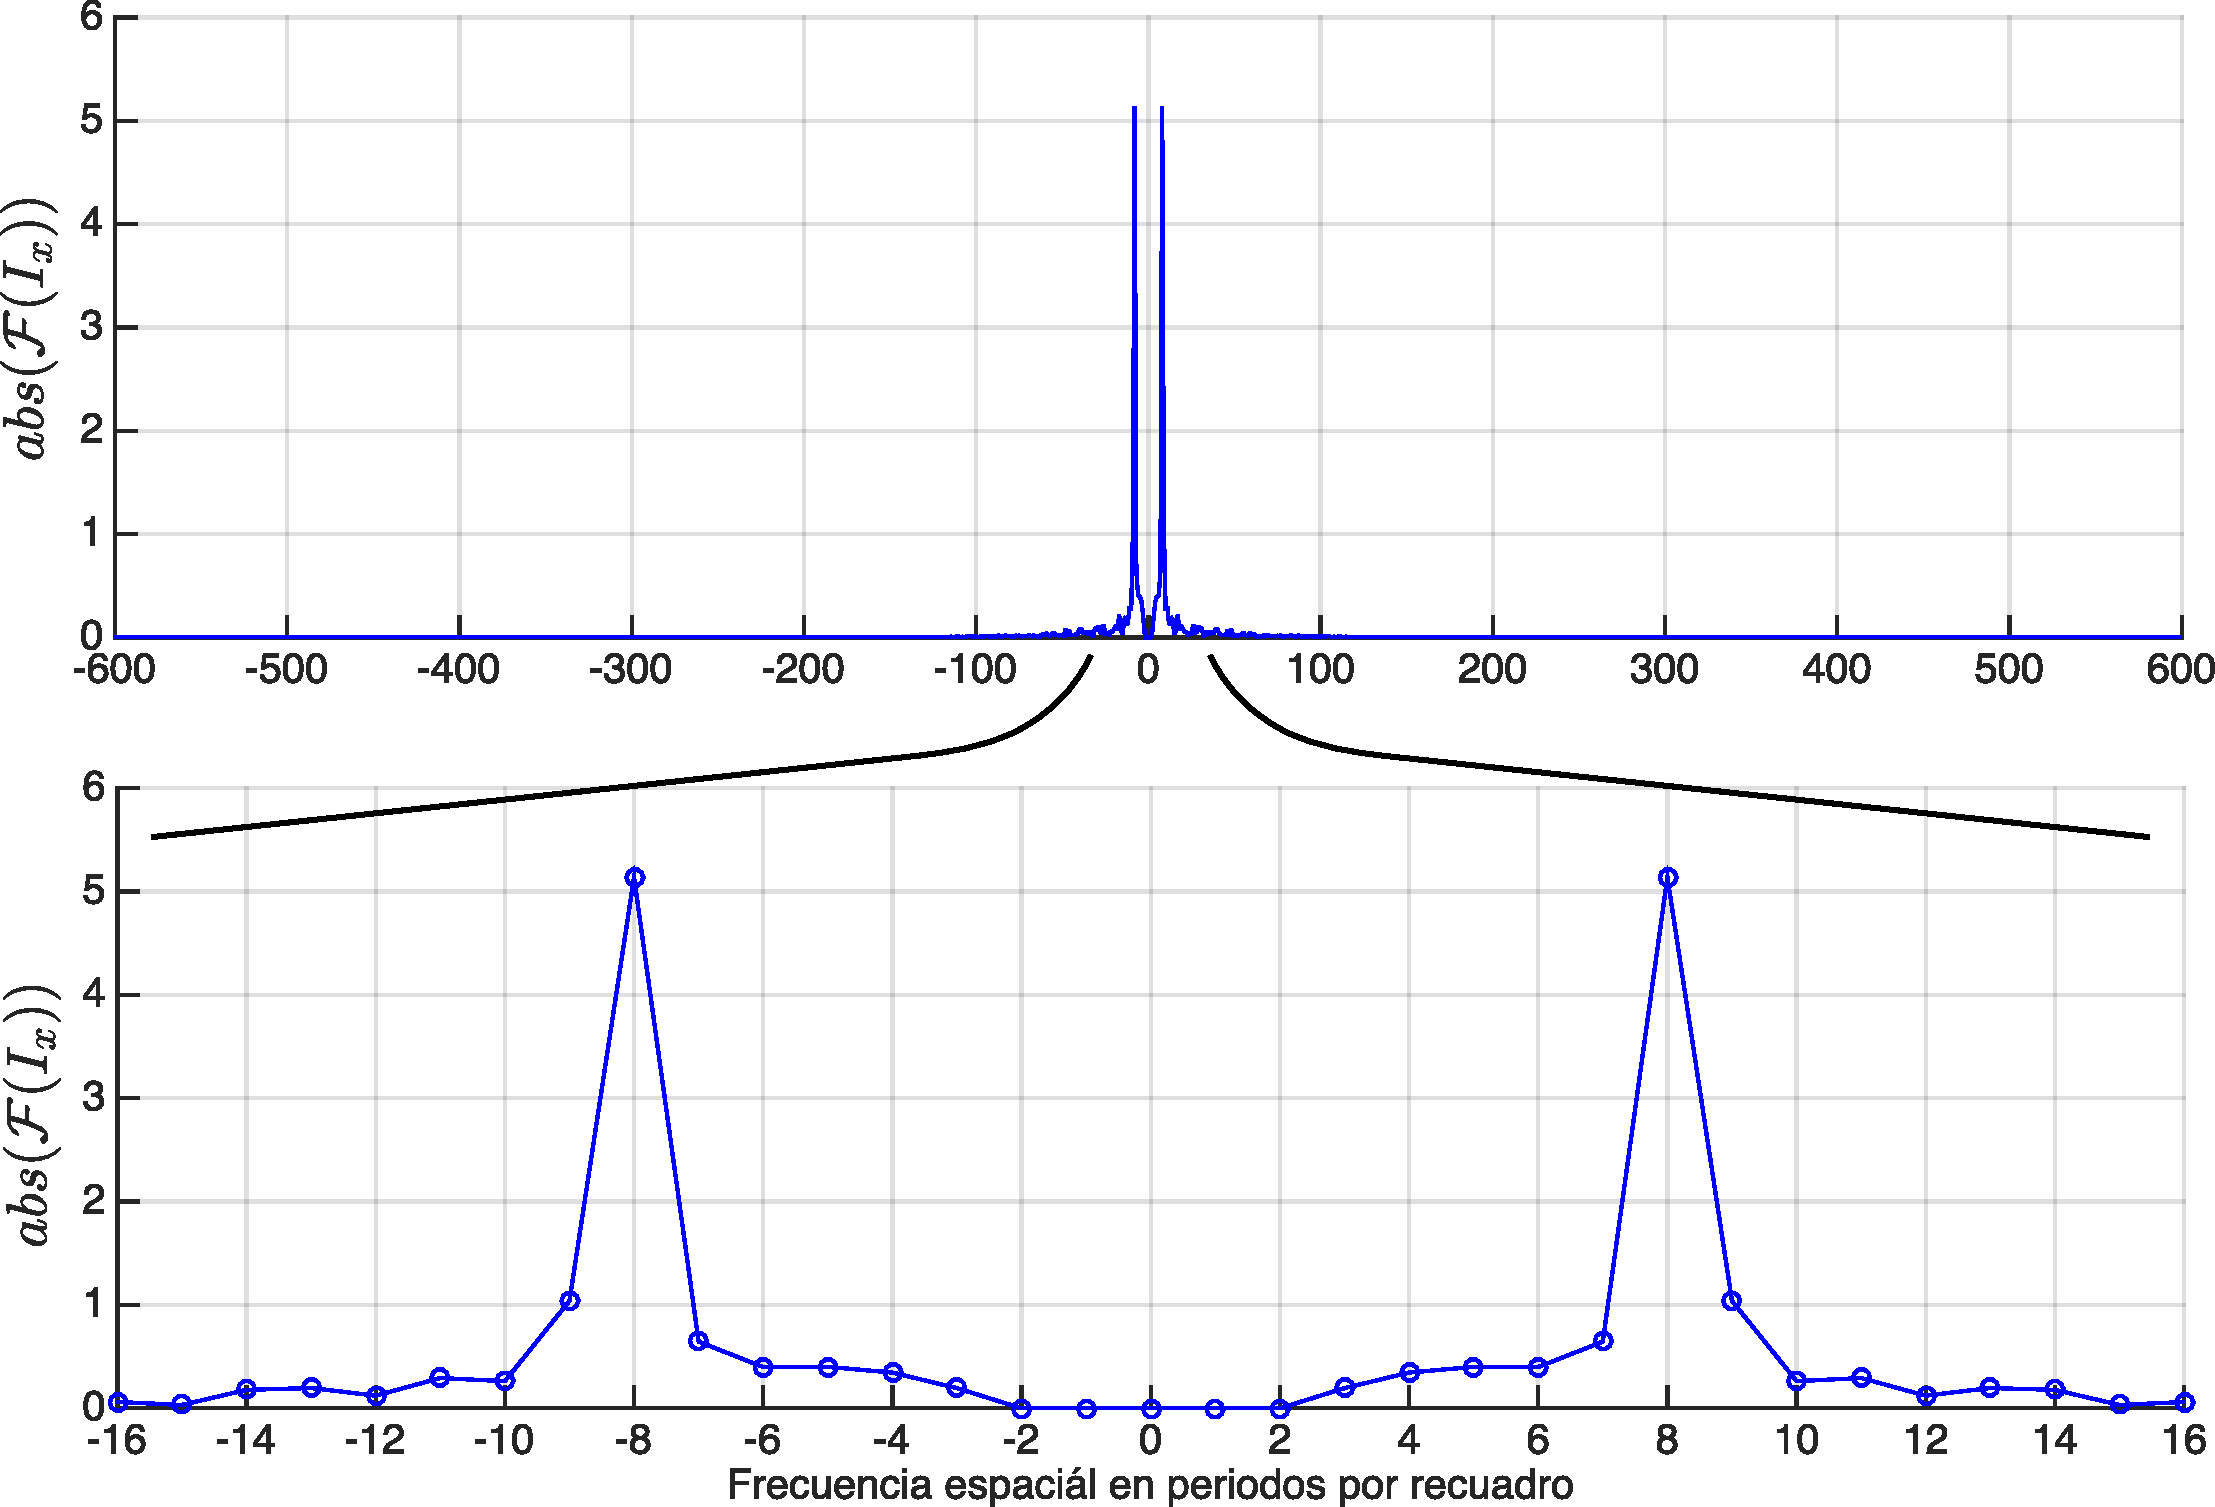
\includegraphics[scale=0.4]{fringes_f_both.pdf}
\caption[Transformada de Fourier de un patrón de
interferencia]{Transformada de Fourier del patrón de interferencia de referencia de la Fig. \ref{fig:fringes_plot}. Como es de
  esperarse para señales sinusoidales hay dos picos simétricos ambos
  lados de la coordenada frecuencial 0. Estos picos señalan correctamente que hay 8
  periodos en el interferograma.}
\label{fig:fringes_f}
\end{figure}
 \begin{figure}[H]
\begin{lstlisting}[style=Matlab]
%  Reference image
imaref=mean(imaref,1);
%  FT scaled 
TFimaref=ifftshift(fft(fftshift(imaref)));
fac=sqrt(1/(size(TFimaref,2)*size(TFimaref,1)));
TFimaref=TFimaref.*fac;
% Filtering of backround peak
radio_mask=2;
TFimaref(:,floor(size(TFimaref,2)/2)+1-radio_mask:floor(size(TFimaref,2)/2)+1+radio_mask)=0;
% Position of max value
[~, IX] = sort(abs(TFimaref),'descend');
% Phase
fase_ref =atan2(imag(TFimaref(1,IX(1))),real(TFimaref(1,IX(1))));
\end{lstlisting}
 \caption{Script para el cálculo de la fase de un interferograma usando
 FT.}
 \label{fig:fourier_script}
 \end{figure}
Si se realiza este proceso para cada una de las dos imágenes se pueden restar las
fases de ambos interferogramas y obtener la diferencia de fase
introducida por un nivel de gris particular. A diferencia del
mencionado anteriormente, este proceso es más preciso y mucho más fácil de implementar en fórma de
un algorítmo que calcule la modulación para cada nivel de gris. 
%\pagebreak
%\subsubsection{Resultados de la medida de modulación de fase}
\subsection{Resultados de la medida de modulación de fase}

Implementando el método de transformadas de Fourier como uno de los
pasos en la caracterización automatizada del SLM, se obtuvieron curvas de modulación
de fase para 60 de los 100 estados mencionados en la sección
\ref{sec:exp_validation}, correspondientes a las polarizaciones de
entrada lineales y circulares.  Las 60 curvas se han puesto al alcance del
lector en el siguiente vínculo web en forma de un notebook de IPython:
\href{http://goo.gl/RtRCX0}{\textbf{http://goo.gl/RtRCX0}}.  

Con estos datos, y con las curvas de modulación de amplitud pudimos
seleccionar una combinaciones de PSD y PSG que tiene condiciones
suficientes para usar el SLM dentro del rango de operación
deseado. Observamos que tal y como se ha reportado en la literatura,
estos moduladores acoplan la modulación de fase con la modulación de
amplitud, y que al menos con nuestro SLM no es posible encontrar
estados en los cuales el SLM sea transparente al variar niveles de gris y al mismo
tiempo permita modulaciones de fase de rango superior a $1.3\pi$.  
Encontramos que el estado 6 (Fig. \ref{fig:amp_and_phase_I6}) produce
modulaciones de fase con rango de modulación muy alto, de casi $1.9\pi$
radianes, y que, sin embargo, está acoplado a una modulación de
intensidad de muy mala calidad en la cual la transmitancia máxima es de
un $60\%$ y se reduce hasta un $10\%$. 
\begin{figure}[H]
\centering
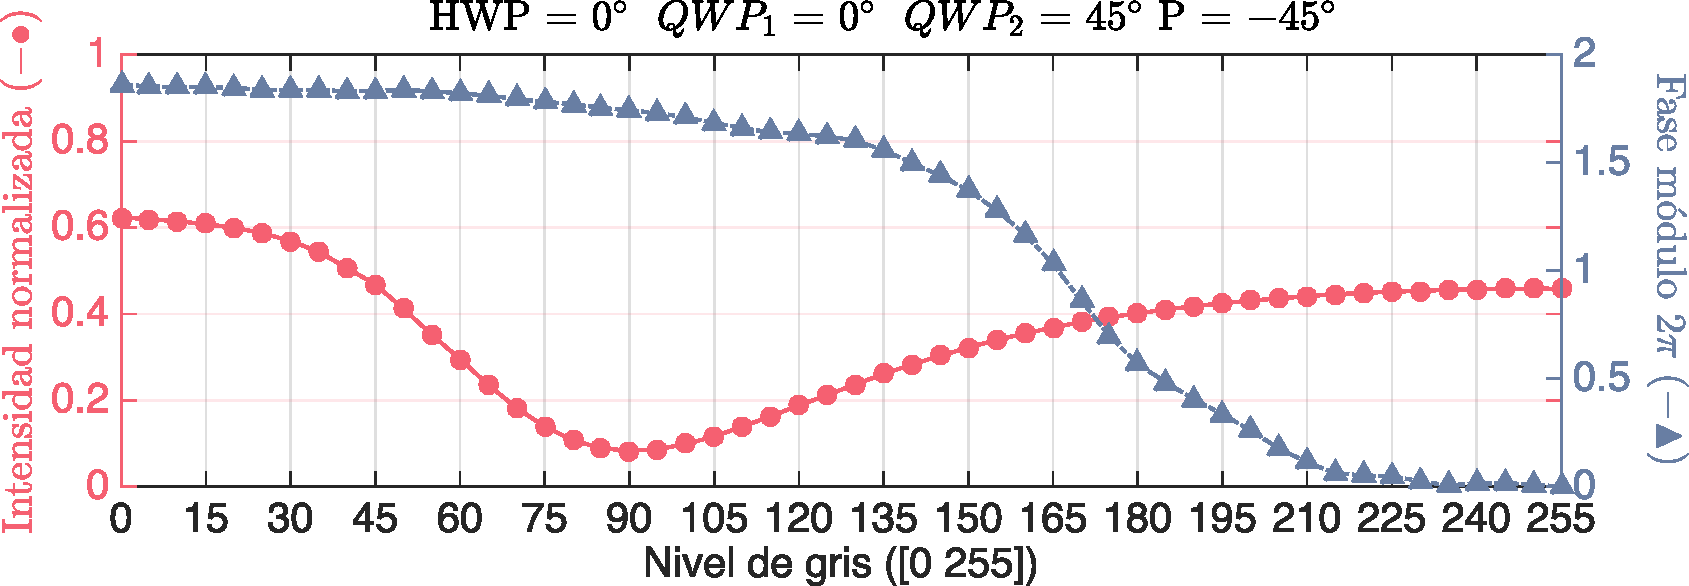
\includegraphics[scale=0.52]{amp_and_phase_I6.pdf}
\caption[Modulación de amplitud y fase del estado con máximo rango de
fase]{Posición de elementos ópticos y curvas de modulación de amplitud
  y fase del BraKet 6 que es el estado con máximo rango de modulación
  fase encontrado.} 
\label{fig:amp_and_phase_I6}
\end{figure}
%Insertar figura con comparación de modulación de amplitud y fase.
Asimismo encontramos varios BraKets en los cuales hay transmitancia
máxima con modulación de amplitud mínima, pero sufren de una muy mala
modulación de fase. Ejemplo de ellos es el BraKet 43
(Fig.~\ref{fig:amp_and_phase_I43}), que tiene alta 
transmitancia, alrededor de $10\%$ de modulación de amplitud y una
 modulación de fase casi nula. Es decir que este SLM es básicamente
 transparente ante la generación y detección estados circulares.
\begin{figure}[H]
\centering
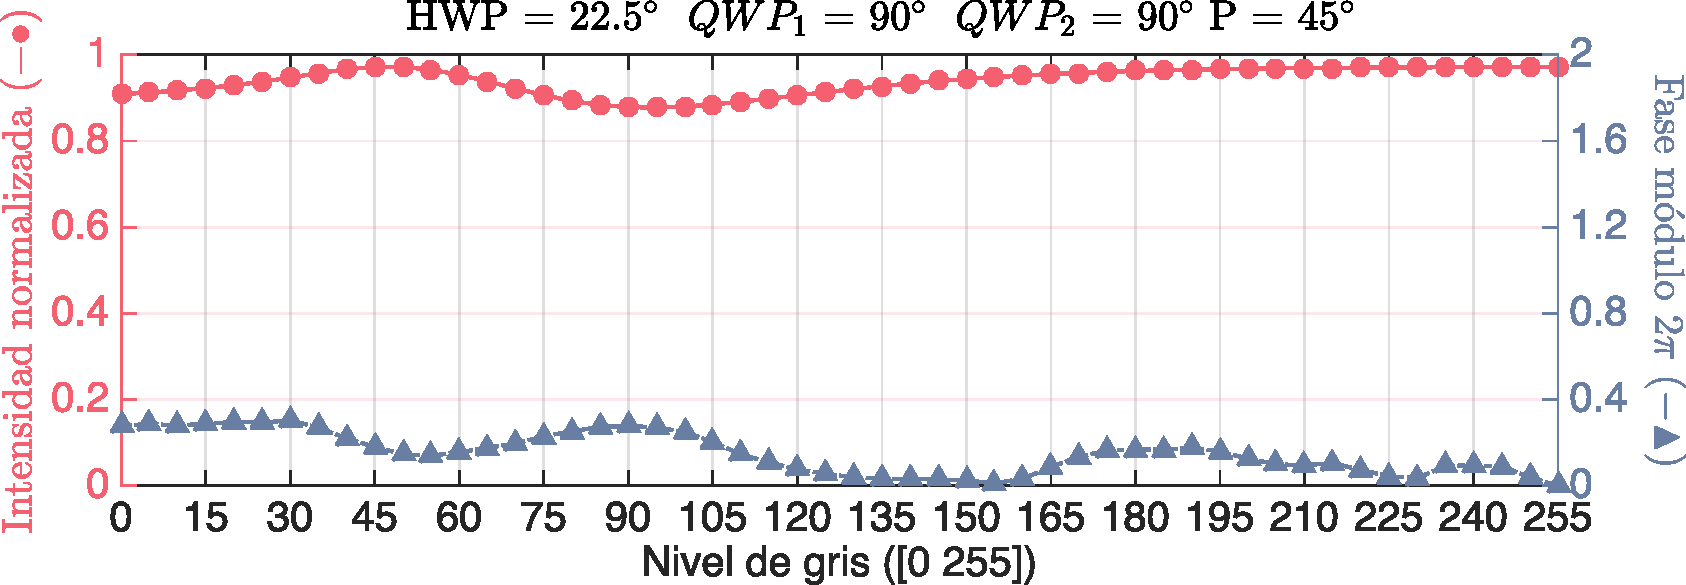
\includegraphics[scale=0.52]{amp_and_phase_I43.pdf}
\caption[Modulación de amplitud y fase del estado con mínima
modulación de amplitud]{Posición de elementos ópticos y curvas de modulación de amplitud
  y fase del BraKet 43 que es uno de los estados con mínimo rango de modulación
  amplitud.} 
\label{fig:amp_and_phase_I43}
\end{figure}

A diferencia de estos puntos extremos, en la configuración que
seleccionamos para la generación de OVs hay un compromiso de uno de
los dos fenómenos. El BraKet seleccionado es el número 10 de la
Fig. \ref{fig:braket_100_notation} que corresponde a un estado
horizontal $\mathbf{H}$ a la entrada y elíptico a $\mathbf{-45^{\circ}}$ a la
salida, las posiciones de los elementos ópticos que lo generan y las
curvas de modulación se presentan en la
Fig. \ref{fig:amp_and_phase_I100}. 
En este estado la transmitancia es baja
($~45\%$) y la modulación de amplitud es relativamente baja ($<20\%$),
pero el rango de modulación de fase es de casi $1.6\pi$ radianes, cosa que como
veremos adelante, resulta suficientemente alta para la generación de
OVs. 
\begin{figure}[H]
\centering
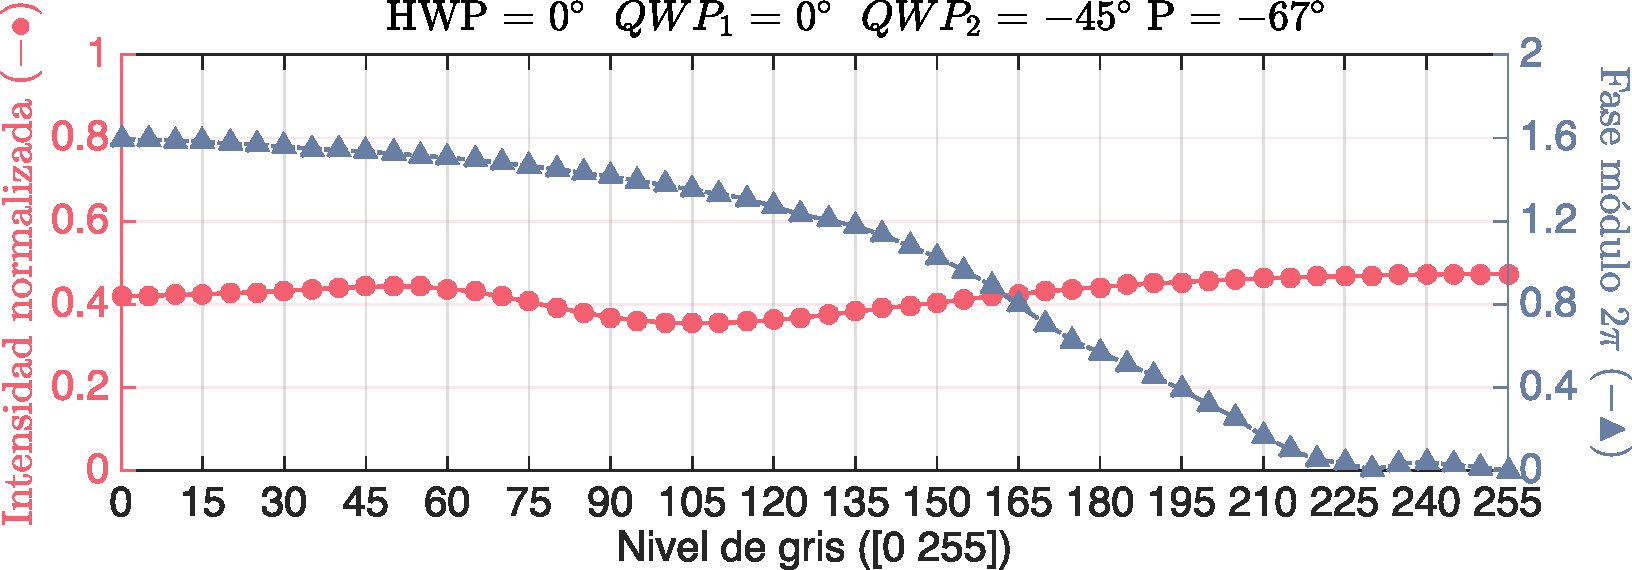
\includegraphics[scale=0.52]{amp_and_phase_I10.pdf}
\caption[Modulación de amplitud y fase óptima]{Posición de elementos
  ópticos y curvas de modulación de amplitud y fase del BraKet 10 que
  se identificó como la configuración óptima para la generación de OVs.} 
\label{fig:amp_and_phase_I100}
\end{figure}

En un principio se pensó que una forma efectiva de encontrar un estado
óptimo podía ser usando un método de minimización similar al que se
usó para encontrar los parámetros de la matriz de Jones. Tál método se
implementó con una función de minimización inspirada en la propuesta
por \citetChGen{Moreno2003} que buscaba simultaneamente
una alta tramitancia, baja modulación de amplitud y alto rango de
modulación de fase. Este planteamiento tiene varios problemas, uno de
ellos es que el espacio de valores de la función para cada
combinación de posibles estados PSG y PSD no es convexo. Es decir que
dependiendo de la semilla usada uno puede obtener un BraKet que
minimice la función de forma local, y que aún así tenga desempeño
regular. Esto se vio en diferentes ocaciones cuando medimos
experimentalmente los BraKets propuestos por las simulaciones. 
Otro problema, es que el tiempo invertido tratando de proponer
manualmente valores de peso que den mayor o menor importancia a la
sensibilidad de los parámetros con respecto a su efecto sobre la
modulación de fase o la de amplitud es excesivo. Generalmente ocurre
que la minimización 
converge a estados circulares que tienen muy buena transmitancia y
baja modulación de amplitud pero mínima modulación de fase. Y si se
modifican ligeramente los factores de peso, la minimización retorna
modulaciones de fase de menos de $1.3\pi$ con modulaciones de amplitud
de entre $15$ y $40\%$. Esto no es mejor al resultado de la
Fig. \ref{fig:amp_and_phase_I100}. Por último, encontramos que las
modulaciones de fase predichas por medio de simulaciones con las
matrices encontradas no predicen con suficiente exactitud muchas de las
modulaciones de fase registradas en el laboratorio. Esto sucede porque los
cambios de estado de polarización introducidos por el SLM afectan el
contraste de las franjas debido a la interferencia destructiva que
sucede con el haz de referencia del interferómetro
Mach-Zehnder. Ante interferogramas como el de la
Fig.~\ref{fig:fringes}(b) el algoritmo de reconstrucción de fase no
tiene como detectar la diferencia de fase entre medidas porque se
pierden las franjas.

Al final, dado que el interés fundamental de este proyecto radicaba en generar
OVs, y no en desarrollar metodos de caracterización, nos resultó mejor
seleccionar el mejor de los 100 estados disponibles (encontrados sin
dificultad por el instrumento de automatización), 
que manipular funciones de peso hasta encontrar un estado simulado con
las condiciones deseadas.

En adelante se mostrará la aplicación que desarrollamos para proyectar
máscaras de fase arbitrarias al SLM, y se mostrarán los OVs que se
pueden generar con un SLM calibrado para la modulación de fase. 

\chapter{Generación de Vórtices Ópticos}
\label{sec:OV_gen}
\label{sec:ChGV_Caracterizacion_de_SLM}
\lhead{Generación de haces Laguerre-Gauss por medio de un SLM:
  \textit{Generación de OVs}}
\section{Introducción}
La mayoría de las fuentes láser tienen cavidades que no son
perfectamente cilíndricas y los campos ópticos que producen o que
prevalecen oscilan en
modos transversales y longitudinales que son solución de la ecuación
de onda en coordenadas cartesianas, dónde las distribuciones de amplitud y fase
del campo óptico pueden ser descritas con por una
combinación de polinomios de Gauss y de Hermite
\citepChGen{Siegman1986}. Esta familia de haces es conocida como
Hermite-Gauss y forma una base completa con la cual se puede describir
cualquier distribución del campo óptico. Asimismo, estos modos son
estructuralmente estables, esto quiere decir que su amplitud y fase
relativa permanecen constantes en la medida en que se propagan en el
campo lejano. Sin embargo, las soluciones Hermite-Gauss de la ecuación de onda
describen solo haces con frentes de onda planos o esféricos, y no dan
cuenta de los frentes de onda helicoidales en los cuales la fase varía
de forma azimutalL; fenómeno macroscópico que está asociado con de la
presencia del \acrshort{OAM} portado por de los fotones que componen
el haz.

Los haces con frente de onda helicoidal también son estructuralmente
estables y han sido producidos desde principios de los 90s. Estos se pueden describir
analíticamente usando las soluciones a la ecuación de onda paraxial en
coordenadas cilíndricas que se presentan en la Eq.~(\ref{eq:Laguerre-Gauss}) \citepChGen{Padgett1999},
\begin{align}
u(r,\phi,z) &\propto \frac{z_R}{(z_R^2+z_R^2)}
\left[\frac{r\sqrt{2}}{w(z)}\right]^lL_p^l\left(\frac{2r^2}{w^2(z)}
\right)\exp{\left(\frac{-r^2}{w^2(z)}\right)}\nonumber\\
&\times \exp{\left(\frac{-ikr^2z}{2(z^2+z_R^2)}\right)}
  \highlightG{\exp(-il\phi)}\exp{\left[i\left(2p+l+1\right)\tan^{-1}\frac{z}{z_R}\right]}
\label{eq:Laguerre-Gauss}
\end{align}
Dónde $L_p^l$ es un \href{http://en.wikipedia.org/wiki/Laguerre_polynomials}{\textbf{polinomio de Laguerre generalizado}} con índices $p$
y $l$, $w(z)$ es el ancho del haz a lo largo de $z$ y
$z_R$ es el
\href{http://www.rp-photonics.com/rayleigh_length.html}{rango de
  Rayleigh}\footnote{Posición en $z$ se cumple la relación $w(z_R)=\sqrt{2}w_0$
  siendo $w_0$ la cintura del spot en el plano focal.}.
La primera línea de la Eq.~(\ref{eq:Laguerre-Gauss}) denota la
amplitud de los haces LG, y la segunda su fase. La combinación de una
componente Gaussiana con los polinomios de Laguerre produce
distribuciones de intensidad que consisten en anillos concentricos
como los que se muestran en la
Fig.~\ref{fig:LG_intensities}.
\begin{SCfigure}[\sidecaptionrelwidth][h!]
\centering
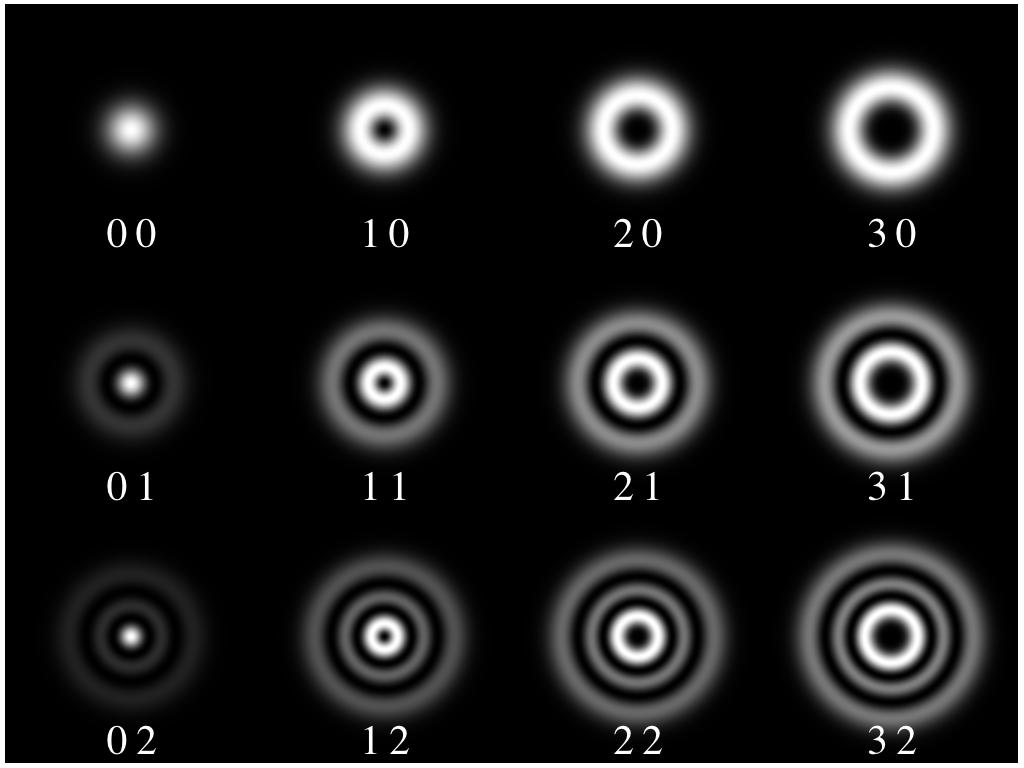
\includegraphics[scale=0.25]{LG-wiki.jpg}
\caption[Primeros
  12 modos LG]{Primeros
  12 modos LG, el caso $0,0$ es equivalente al modo $0,0$ de la base
  Hermite-Gauss. En adelante se considerarán solamente los VOs con un
  sólo anillo es decir, número $p=0$. Imágen con licencia
  \href{https://creativecommons.org/licenses/by-sa/3.0/}{\textbf{CC-BY-SA-3.0}}
    tomada de Wikimedia, autor original Ziofil.} 
\label{fig:LG_intensities}
\end{SCfigure}

En cuanto a la fase, se puede identificar que además de la fase
sociada a frentes de onda esféricos que depende de $r$,
hay dos terminos exponenciales complejos nuevos que tienen como
argumento los índices $l$ y $p$. El último exponencial describe las variaciones de
la fase a lo largo de la dirección de propagación, y el primero, que
hemos resaltado en verde, y depende del número $l$ solamente, describe
los cambios azimutales de la fase.
Nos referiremos a la expresión $\exp(-il\phi)$ como la fase espiral, y
además de ser la responsable de las distribuciónes
de fase helicoidal de los haces LG, está asociada al \acrshort{OAM} que
portan sus fotones. El número $l$ se conoce como la \textbf{carga topológica} de
la singularidad en el VO y determina la cantidad de veces que la fase
varía de $0$ a $2\pi$ alrededor del eje óptico. La representación de
las fases espirales y los perfiles de amplitud de haces LG con
diferentes cargas topológicas se ilustran en la Fig.~\ref{fig:spirals}
y se puede
observar que VOs de mayor carga
topológica tienen mayor tamaño y una región oscura más grande.
\begin{SCfigure}[\sidecaptionrelwidth][h!]
\centering
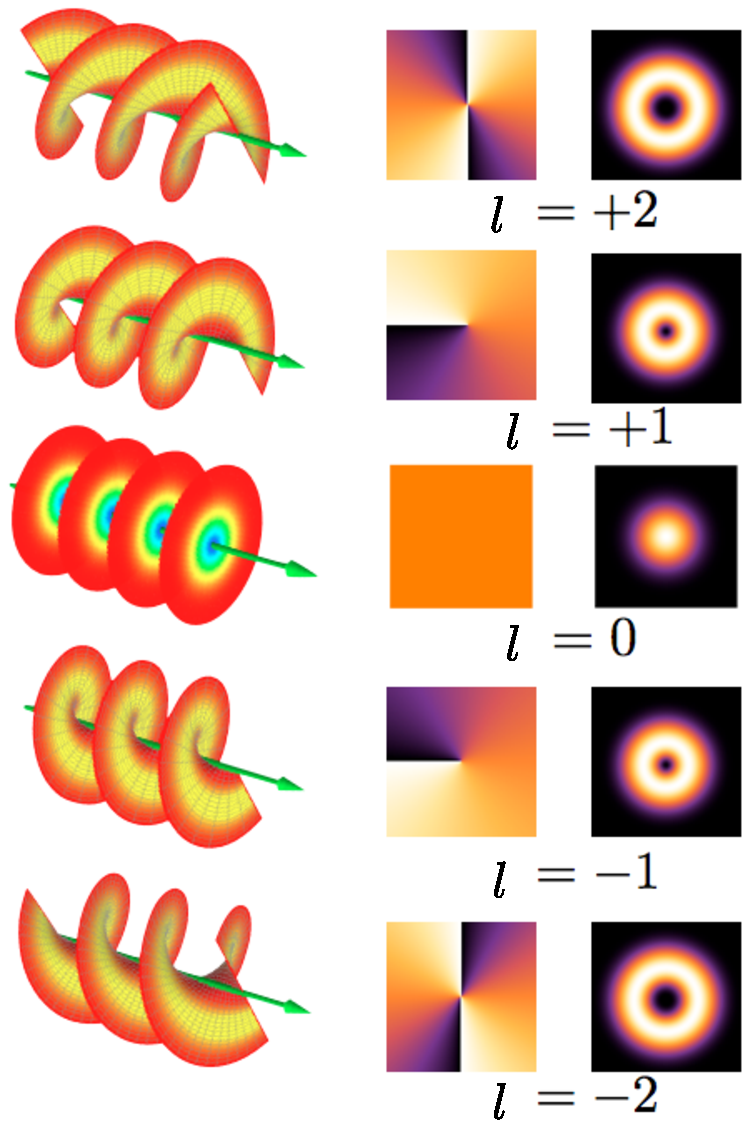
\includegraphics[scale=0.5]{spirals.pdf}
\caption[Fase e intensidad de haces LG]{Propagación de la
  fase, y mapas dos de la intensidad y frente de onda de haces LG con
  carga topológica 
  $l=-2:2$ y número $p =0$. El signo de $l$ determina tanto el sentido
  de giro de la fase como el signo del OAM que porta el haz. VOs con
  mayor $l$ tienen anillos más grandes. Imágen con licencia
  \href{https://creativecommons.org/licenses/by-sa/3.0/}{\textbf{CC-BY-SA-3.0}}
    tomada de Wikimedia, autor original E-karimi.} 
\label{fig:spirals}
\end{SCfigure}

Como se mencionó en la Sección \ref{sec:ChGen_marco_teorico}, para generar un haz
Laguerre-Gauss sólo basta propagar un haz gausiano por una máscara de
fase espiral como la de la Fig.~\ref{fig:oam_intro}b) para que
adquiera las distribuciones de fase de la
Fig.~\ref{fig:spirals}. Haciendo esto, los perfiles de
intensidad de la primera línea de la  Fig.~\ref{fig:LG_intensities}
pueden ser observados en un plano imagen como una \textbf{función de dispersión de punto} (\acrshort{PSF}) si se añade una lente
al brazo objeto del montaje de la Fig.~\ref{fig:oam_intro}.  

En este capítulo presentaremos una plataforma computacional que
desarrollamos en el contexto de este proyecto para
generar máscaras de fase que al ser  proyectadas en un SLM con
suficiente rango de modulación de fase, convierten
un haz Gausiano en un haz LG.

\section{Plataforma computacional para la generación de máscaras de fase}

Con el objetivo de facilitar la creación y manipulación de máscaras de
fase se agruparon en una sola aplicación gráfica los algoritmos para
generación de máscaras de amplitud 
y fase desarrollados durante el transcurso de este proyecto. Esta aplicacion
ha sido desarrollado en el entorno Matlab$\circledR$ y se encuentra en
proceso una aplicación de registro de software ante la Dirección
Nacional de Derecho de Autor.
Una captura de pantalla del panel de control de la aplicación se muestra en la Fig.~\ref{fig:mask_app}, y la
generación de máscaras espiral de fase, como la que se ve en el
recuadro izquierdo del recorte, se logra haciendo click en el botón
``Generate mask'' previamente seleccionado un valor de
carga topológica en la primera casilla titulada ``SpiralMask''. 
\begin{figure}[h!]
\centering
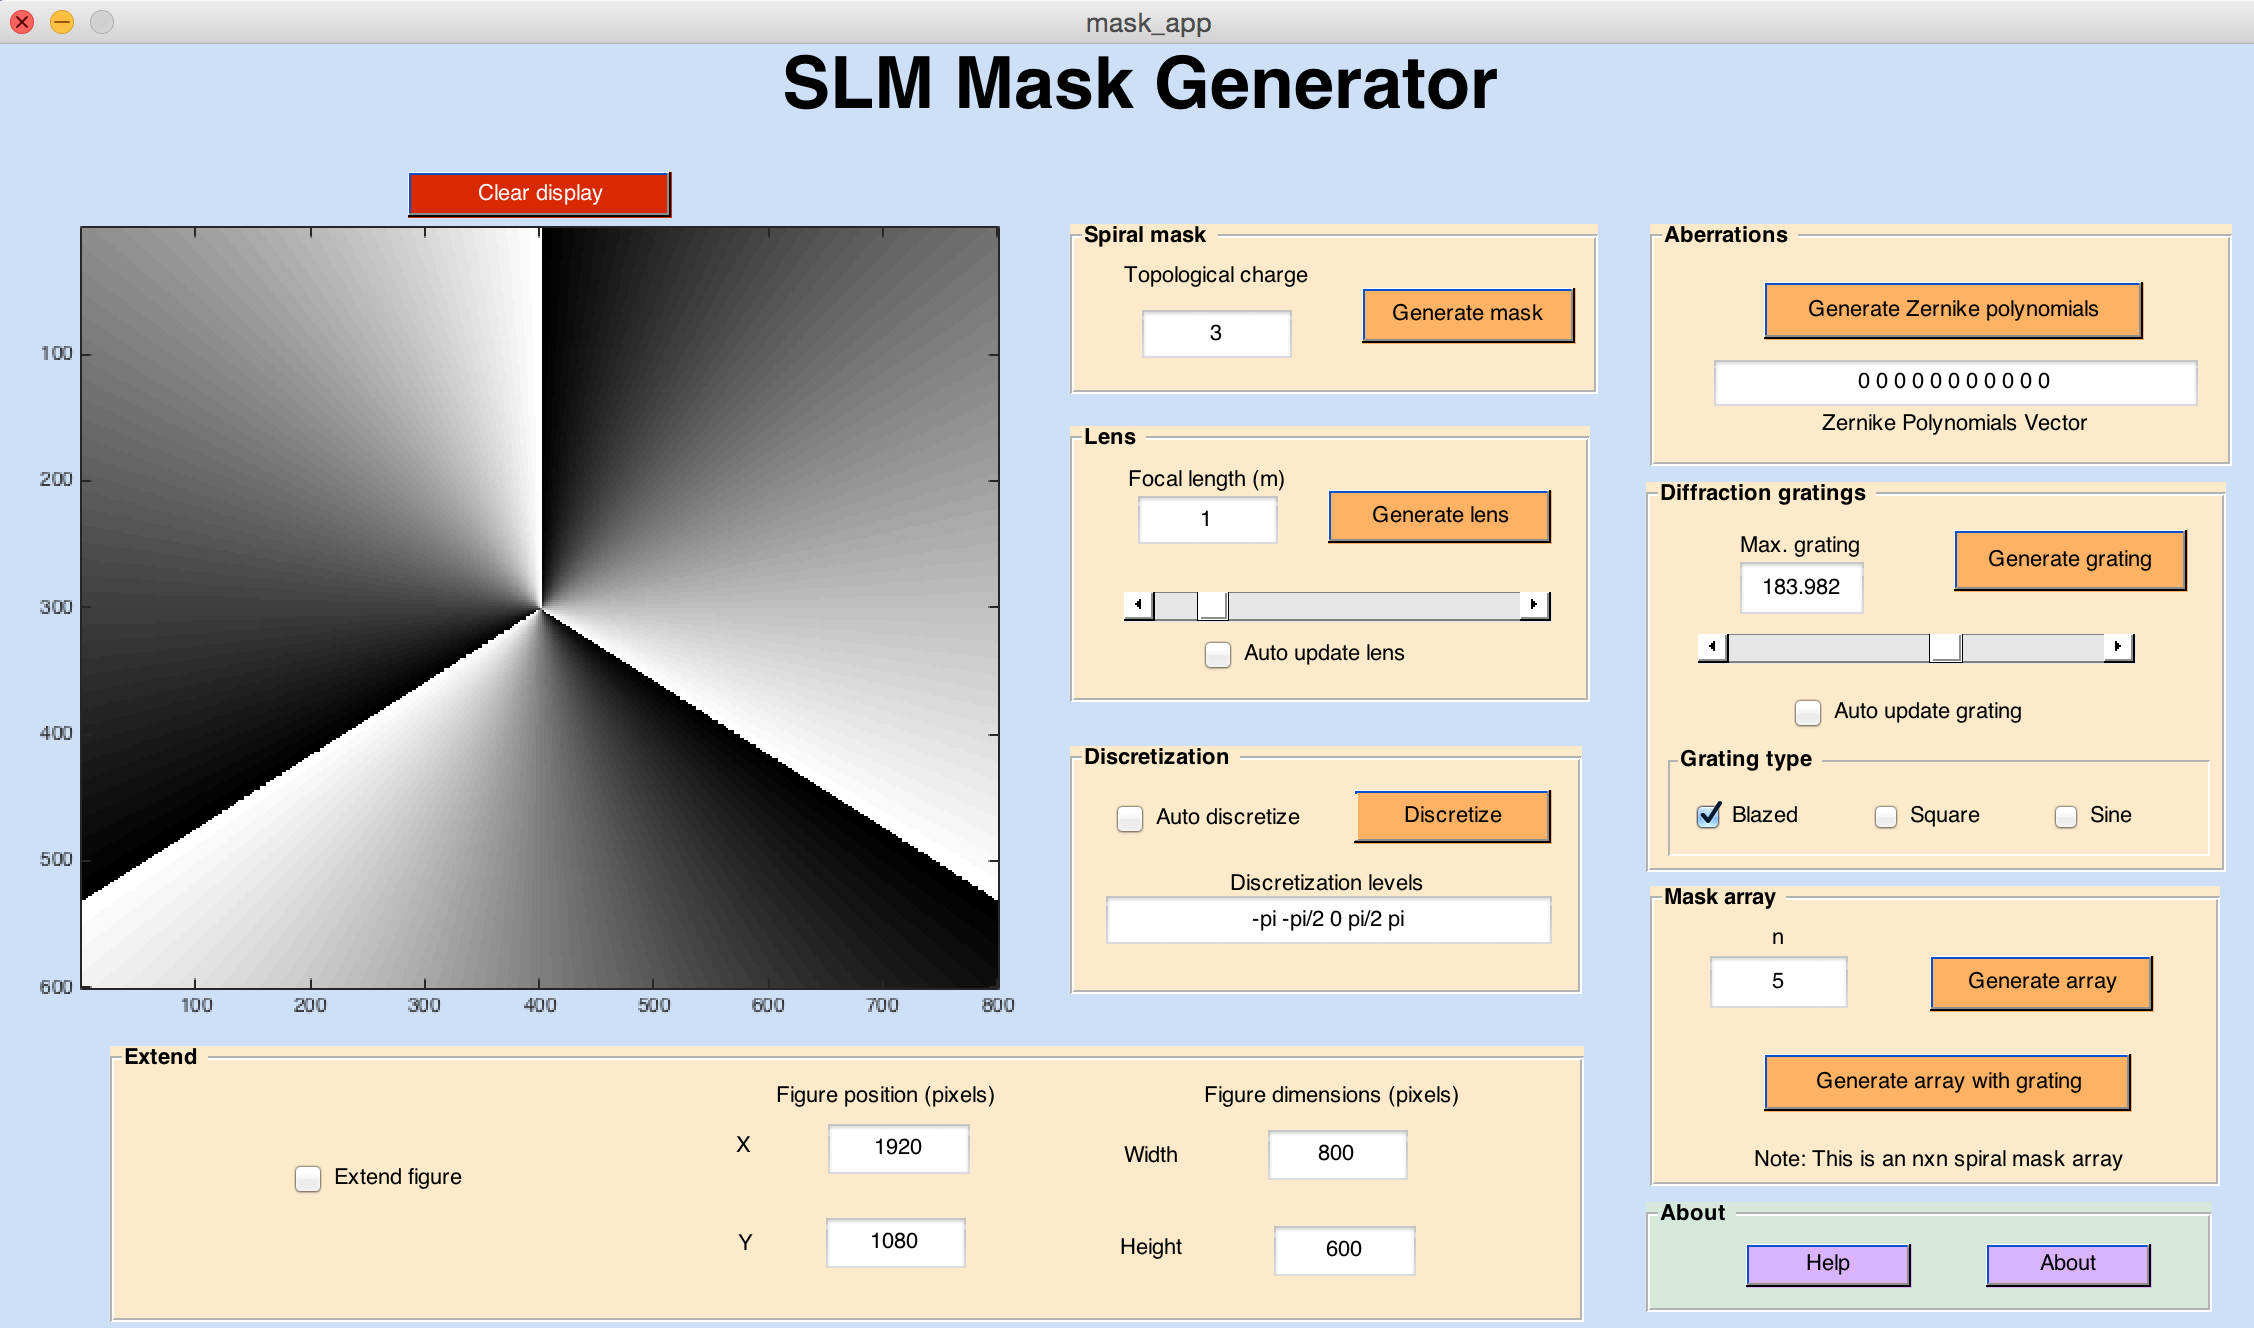
\includegraphics[scale=0.4]{mask_app.png}
\caption[Plataforma para la generación de máscaras de fase]{Plataforma
  para la generación de máscaras de fase a ser proyectadas en un SLM. Desarrollada y registrada por el
  grupo de Óptica Aplicada de la Universidad EAFIT.} 
\label{fig:mask_app}
\end{figure}

Los SLMs que han sido conectados a un computador actúan como una segunda
pantalla y para llevar la máscara generada a la región del escritorio
correspondiente al LCD del SLM se usa el recuadro titulado ``Extend'' ubicado
en la parte inferior de la aplicación. La máscara espiral de fase de
carga $l=3$ que ha sido previsualizada en el recuadro izquierdo de la
Fig.~\ref{fig:mask_app} puede
ser proyectada o extendida al SLM haciendo click en la casilla
titulada ``Extend figure'' y seleccionando el tamaño y posición en 
píxeles donde se desea ubicar la imágen.  

Además de generar máscaras espiral, la aplicación permite reducir el
número de niveles de gris de la modulación para implementar métodos
como los de \citetChGen{Londono2015} o \citetChGen{Rueda2013} y simular
otros tipos de elementos de fase como: lentes de Fresnell, aberraciones
parametrizadas en la base de polinomios de Zernike\footnote{Ver apéndice
  \ref{cha:Anexo3} dónde se introducen los polinomios de Zernike y la
  composición de aberraciones en su base}, rejillas de difracción de
tres tipos distintos e
inclusive arreglos de máscaras.

A continuación se muestran los resultados de la propagación de haces
Gaussianos a través de máscaras espiral de fase de distinto $l$
proyectadaes en el SLM. 

\section{Resultados de los Vórtices Ópticos obtenidos}

En la Fig.~\ref{fig:VOs_I10} se presentan las distribuciones de
intensidad correspondientes a la generación de VOs con máscaras de
fase espiral de carga topológica $l=1:5$ usando el SLM con la
combinación de PSG y PSD del BraKet 10 que tiene las modulaciones de
la Fig.~\ref{fig:amp_and_phase_I100}. 
\begin{figure}[h!]
\centering
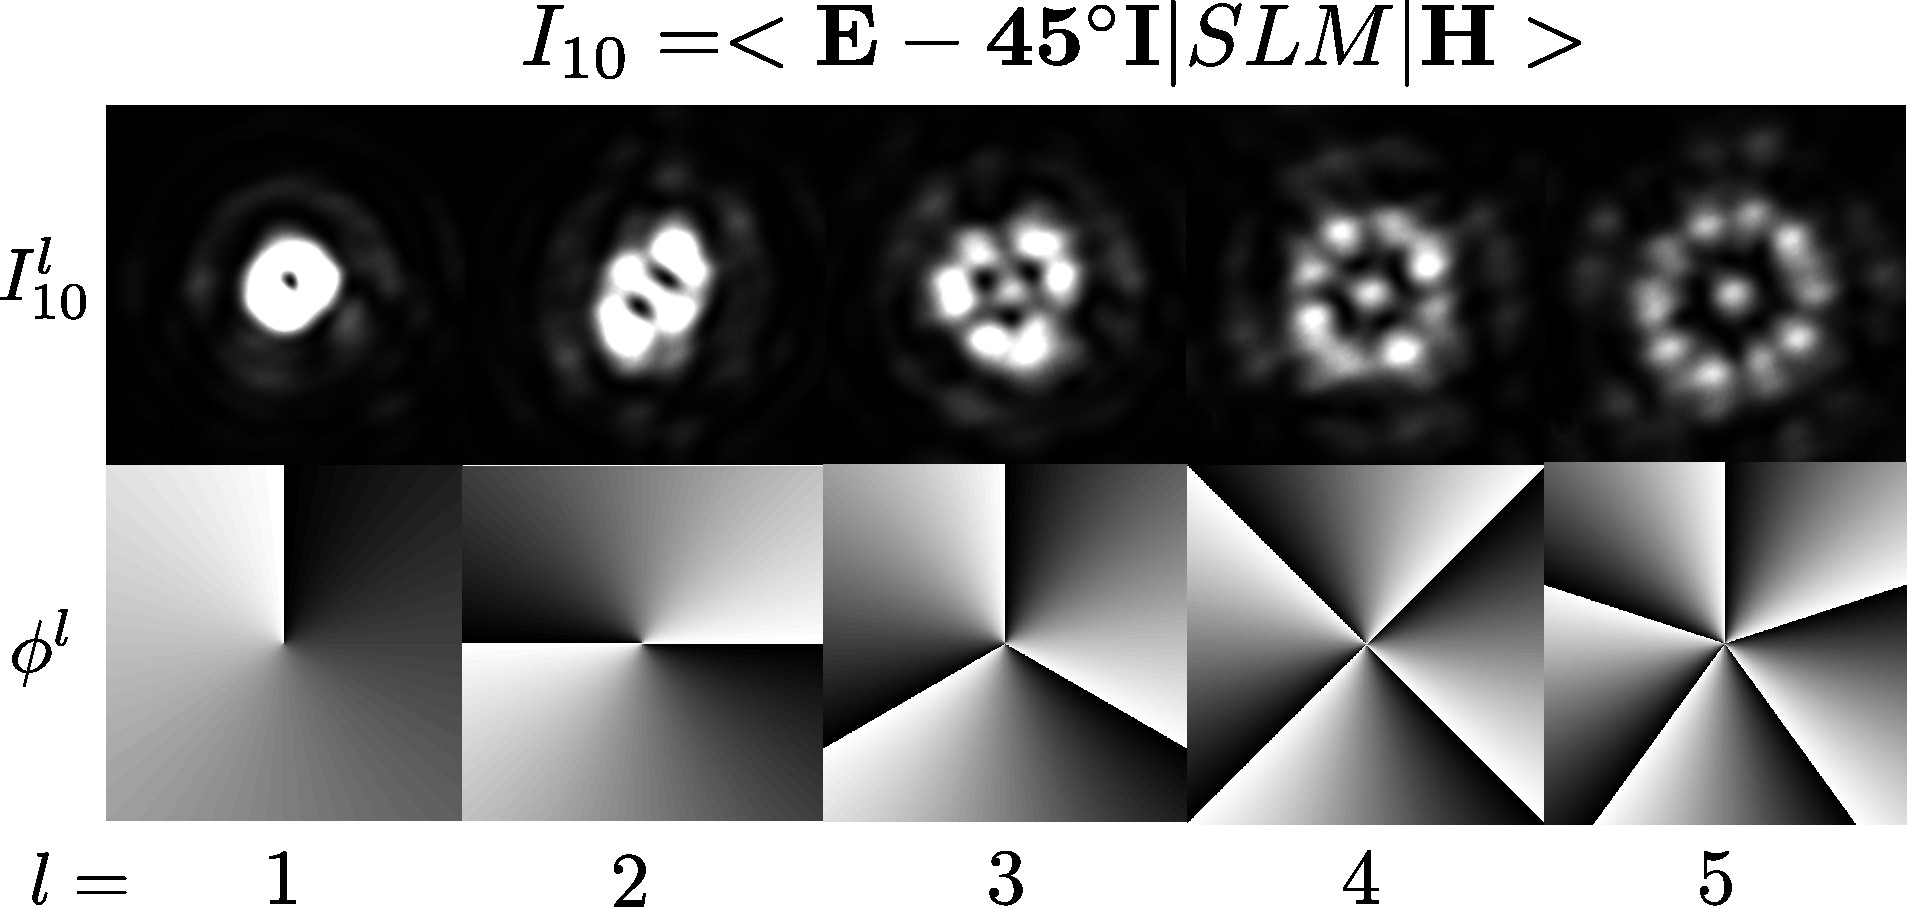
\includegraphics[scale=0.4]{OV_I10.pdf}
\caption[Vórtices ópticos obtenidos en la configuración en linea para
el BraKet 10]{Vórtices ópticos de carga topológica $l=1:5$ obtenidos
  en la configuración en linea usando los estados PSG y PSD del BraKet 10.} 
\label{fig:VOs_I10}
\end{figure}
De inmediato se puede ver que sólo el primero de ellos tiene la
topología típica de un VO, y que a lo largo del anillo varía la
intensidad con unas partes más intensas que otras. El hecho de que
sólo se pueda producir el VO con $l=1$ se debe en parte a las
aberraciones ópticas del sistema que destruyen las singularidades de
carga alta y en parte al hecho de que no se
lograron rangos de modulación de $2\pi$ con el SLM. En particular se
puede notar que la forma de la aberración presente en el VO
con carga topológica $l=2$ indica que hay una componente importante de
astigmatismo, muy similar al comportamiento de las reportadas por \citetChGen{Singh2008} \textit{et~al.}. Por otra parte, la
no uniformidad de la intensidad en el anillo se debe a que
la modulación de amplitud no es constante para todos los niveles de
gris. 

Ahora bien, cabe notar que estos resultados se han logrado con el
estado que tiene la mejor combinación de modulación de amplitud plana
y fase amplia. Hemos observado que si se usara el SLM con estados de
polarización diferentes no se obtendría ni siquiera el VO de
$l=1$. Como ejemplo, en la \ref{fig:VOs_I6} se presentan las
distribuciones de intensidad equivalente cuando se usan los estados de
polarizaci'on del BraKet 6. 
\begin{figure}[h!]
\centering
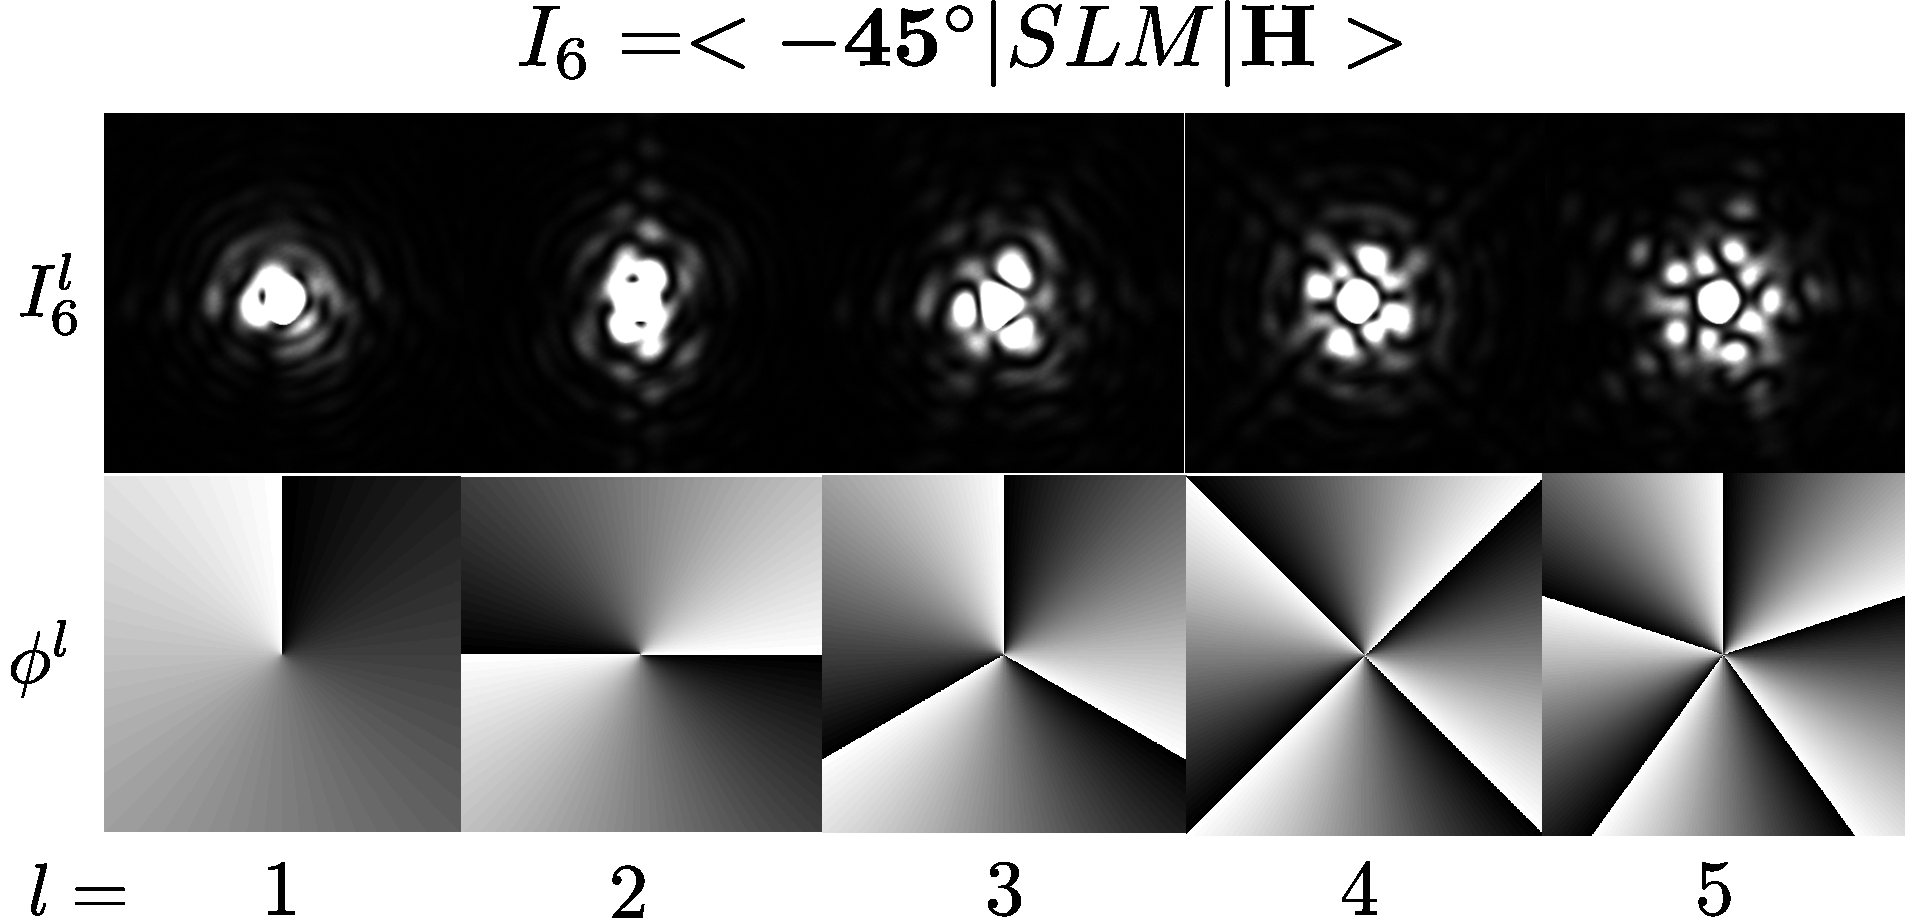
\includegraphics[scale=0.4]{OV_I6.pdf}
\caption[Vórtices ópticos obtenidos en la configuración en linea para
el BraKet 6]{Vórtices ópticos de carga topológica $l=1...5$ obtenidos
  en la configuración en linea usando los estados PSG y PSD del BraKet 6.} 
\label{fig:VOs_I6}
\end{figure}
En este caso, la distribución de la intensidad se asemeja a la PSF de
un sistema con grandes aberraciones y predomina la intensidad de la
luz que no fue difractada por la máscara de fase. 

Sin embargo, hay una forma de mejorar la calidad de la modulación de
ambos estados que
consiste en agregar una red de difracción a la máscara espiral. A
continuación se describe este método y se presentan los VOs generados
al utilizar esta modificación. 

\subsection{Vótices Ópticos obtenidos usando máscaras tipo tenedor}

En la literatura, los VOs generados con máscaras espiral se conocen
como \textit{``en línea''}. Esto quiere decir que toda la luz que pasa
por el SLM se observa en el plano imagen. Esto es positivo si el SLM
tiene un muy buen rango de modulación, si es importante tener una
buena cantidad de luz o si el diseño del instrumento que genera VOs no
permite sacar el haz de eje. Sin embargo, en la práctica rara vez es usada esta
configuración pues sacar los VOs de eje usando una red de difracción
de tipo tenedor mejora sustancialmente la calidad óptica al reducir la
interferencia con la luz no difractada\citepChGen{Maurer2011}.
Según \citetChGen{Leach2004}, igual que con elementos difractivos
convencionales, las imperfecciones en la linealidad de la fase y otros
fenómenos que disminuyen la eficiencia como: efectos de difracción en los saltos de fase, el área no
efectiva de las celdas o la
periodicidad de los píxeles, significan
que la luz que atraviesa el SLM es difractada en un número
significativo de ordenes de difracción. Si estos ordenes se
superponen, como es el caso del haz observado en un montaje \textit{en línea} resulta
una versión deteriorada del haz esperado. Esto puede explicar los
resultados presentados en las Fig.~\ref{fig:VOs_I10}
y\ref{{fig:VOs_I6}}. Es por esto que autores clásicos de los
inicios del estudio de VOs como 
\citetChGen{Bazhenov1990}, \citetChGen{Leach2004}, y
\citetChGen{Dennis2009}  han propuesto usar máscaras de fase conocidas
como \textit{mascaras tenedor} que se ilustra en la
Fig.~\ref{fig:fork_recipe}(c) y son rejillas de difracción con
dislocaciones en su centro. Las máscaras del tipo tenedor resultan de la combinación de una
máscara espiral y un plano inclinado o rejilla de difracción y el
efecto que tienen sobre un haz Gaussiano de entrada es el de producir VOs de
carga topológica $m\times l$ difractados a un ángulo fuera de eje que
depende del órdenes de
difracción $m$ donde se observe, de la longitud de onda y de la distancia.
\begin{figure}[h!]
\centering
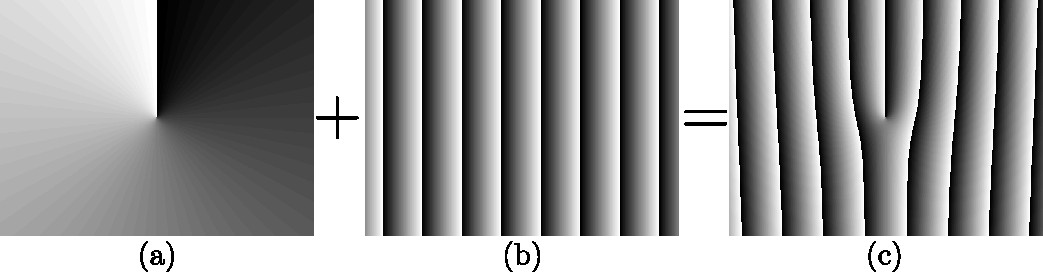
\includegraphics[scale=.7]{fork_recipe.pdf}
\caption[Composición de una máscara tipo tenedor con dislocación de
carga 1]{La suma de una máscara espiral de fase (a) con una máscara de
una rejilla de difracción (b) produce una máscara del tipo tenedor
(c) con una dislocación del mismo valor que la carga topológica de la
espiral original.} 
\label{fig:fork_recipe}
\end{figure}

En un principio, una rejilla de difracción como la de la
Fig.~\ref{fig:fork_recipe}(b)
emula una cuña delgada y es capaz de difractar toda la energía
incidente en el primer orden\citepChGen{Dennis2009}. Sin embargo, en la
práctica este nunca es el caso y una fracción de la energía queda en
los otros ordenes, esto implica una menor eficiencia y la nececidad de
filtrar o seleccionar sólo el orden de difracción deseado que porta el
VO a ser detectado. Aunque hay un gran incremento en la calidad de los
VOs generados con rejillas de este tipo algunos posibles
inconvenientes son: la necesidad de trabajar con luz monocromática
para evitar aberración cromática, y las limitantes geométricas que
implica el tener que sacar el haz de eje y filtrar las otras
componentes. 

Como nosotros usamos una fuente de iluminación monocromática y no
tenemos problemas de espacio, decidimos implementar el montaje fuera
de eje para mejorar la calidad de los VOs obtenidos. Los resultados de
VOs generados con rejillas del tipo tenedor para las configuraciones
de polarización de los BraKets 10 y 6 se presentan en la
Fig.~\ref{fig:diffracted_OV_I6_and_I10}. El montaje con el cual fueron
generados es un sistema formador de imagen del tipo 4F que se ilustra
en la Fig.~\ref{fig:exp_setup} 
y se discute en el siguiente capítulo en la Sección \ref{sec:montaje_PD}. 
\begin{figure}[h!]
\centering
\includegraphics[scale=0.3]{diffracted_OV_I6_and_I10.pdf}
\caption[Vórtices ópticos difractados por una rejilla tipo
blazed.]{Comparación de Vórtices ópticos de carga topológica $l=1...4$ obtenidos en
  la configuración fuera de linea al usar una máscara tipo tenedor
  cuando se ubican los elementos ópticos que generan los estados PSG y PSD de los
  BraKets 10 y 6.} 
\label{fig:diffracted_OV_I6_and_I10}
\end{figure}

Se observa inmediatamente que con las máscaras tenedor se forman VOs
con estructuras aceptables en ambas
configuraciones, y para todos los valores de carga topológica. Además,
se confirma que el BraKet 10 es una combinación de
estados de polarización con muy alta eficiencia de difracción ya que
la mayor parte de la luz es difractada en el orden 1. En cambio, los
VOs en el orden 1 obtenidos en la configuración 6 tienen una
intensidad que es menor a la de la luz no difractada que se concentra
en el orden 0. Intensidad que es típica de un sistema formador de
imagen sin máscaras. Ambos estados comparten la característica de
tener altos rangos de modulación de fase ($>1.5$) pero sólo con el que
tiene buena modulación de amplitud es posible lograr VOs en linea. 

Una característica de los VOs de cargas mayor a 1 es que tienden a
separarse en varios VOs de carga 1 ante la presencia de
aberraciones. Esto se puede observar con claridad en los VOs de carga
$l=2$ de las Fig.~\ref{fig:VOs_I10} y
\ref{fig:diffracted_OV_I6_and_I10} dónde se hace evidente que hay al menos una componente
de astigmatismo.  En lo que sige de esta disertación se presenta un
método de caracterización y corrección de aberraciones con el cual es
posible mejorar la calidad de VOs producidos en sistemas formadores de
imagen. 

\newpage
\pagebreak[4]
\bibliographystyleChGen{ezspanish}
\bibliographyChGen{References/Ch2}t